%% Copernicus Publications Manuscript Preparation Template for LaTeX Submissions
%DIF LATEXDIFF DIFFERENCE FILE
%DIF DEL anterior.tex   Mon May 27 22:51:28 2019
%DIF ADD template.tex   Mon May 27 22:44:35 2019
%% ---------------------------------
%% This template should be used for copernicus.cls
%% The class fil e and some style files are bundled in the Copernicus Latex Package which can be downloaded from the different journal webpages.
%% For further assistance please contact the Copernicus Publications at: publications@copernicus.                                                                                         x    
%% http://publications.copernicus.org


%% Please use the following documentclass and Journal Abbreviations for Discussion Papers and Final Revised Papers.


%% 2-Column Papers and Discussion Papers
%++++++++++++++++++++++35\documentclass[nhess, manuscript]{copernicus}
%\documentclass[nhess]{copernicus}
\documentclass[hess, manuscript]{copernicus}


%% Journal Abbreviations  (Please use the same for Discussion Papers and Final Revised Papers)

% Atmospheric Chemistry and Physics (acp)
% Advances in Geosciences (adgeo)
% Advances in Statistical Climatology, Meteorology and Oceanography (ascmo)
% Annales Geophysicae (angeo)
% ASTRA Proceedings (ap)
% Atmospheric Measurement Techniques (amt)
% Advances in Radio Science (ars)
% Advances in Science and Research (asr)
% Biogeosciences (bg)
% Climate of the Past (cp)
% Drinking Water Engineering and Science (dwes)
% Earth System Dynamics (esd)
% Earth Surface Dynamics (esurf)
% Earth System Science Data (essd)
% Fossil Record (fr)
% Geographica Helvetica (gh)
% Geoscientific Instrumentation, Methods and Data Systems (gi)
% Geoscientific Model Development (gmd)
% Geothermal Energy Science (gtes)
% Hydrology and Earth System Sciences (hess)
% History of Geo- and Space Sciences (hgss)
% Journal of Sensors and Sensor Systems (jsss)
% Mechanical Sciences (ms)
% Natural Hazards and Earth System Sciences (nhess)
% Nonlinear Processes in Geophysics (npg)
% Ocean Science (os)
% Primate Biology (pb)
% Scientific Drilling (sd)
% SOIL (soil)
% Solid Earth (se)
% The Cryosphere (tc)
% Web Ecology (we)



%% \usepackage commands included in the copernicus.cls:
%\usepackage[german, english]{babel}
%\usepackage{tabularx}
%\usepackage{cancel}
%\usepackage{multirow}
%\usepackage{supertabular}
%\usepackage{algorithmic}
%\usepackage{algorithm}
%\usepackage{float}
%\usepackage{subfig}
%\usepackage{rotating}
\usepackage{color}
\definecolor{mypink}{RGB}{219, 48, 122}
%DIF PREAMBLE EXTENSION ADDED BY LATEXDIFF
%DIF UNDERLINE PREAMBLE %DIF PREAMBLE
\RequirePackage[normalem]{ulem} %DIF PREAMBLE
\RequirePackage{color}\definecolor{RED}{rgb}{1,0,0}\definecolor{BLUE}{rgb}{0,0,1} %DIF PREAMBLE
\providecommand{\DIFadd}[1]{{\protect\color{blue}\uwave{#1}}} %DIF PREAMBLE
\providecommand{\DIFdel}[1]{{\protect\color{red}\sout{#1}}}                      %DIF PREAMBLE
%DIF SAFE PREAMBLE %DIF PREAMBLE
\providecommand{\DIFaddbegin}{} %DIF PREAMBLE
\providecommand{\DIFaddend}{} %DIF PREAMBLE
\providecommand{\DIFdelbegin}{} %DIF PREAMBLE
\providecommand{\DIFdelend}{} %DIF PREAMBLE
%DIF FLOATSAFE PREAMBLE %DIF PREAMBLE
\providecommand{\DIFaddFL}[1]{\DIFadd{#1}} %DIF PREAMBLE
\providecommand{\DIFdelFL}[1]{\DIFdel{#1}} %DIF PREAMBLE
\providecommand{\DIFaddbeginFL}{} %DIF PREAMBLE
\providecommand{\DIFaddendFL}{} %DIF PREAMBLE
\providecommand{\DIFdelbeginFL}{} %DIF PREAMBLE
\providecommand{\DIFdelendFL}{} %DIF PREAMBLE
%DIF END PREAMBLE EXTENSION ADDED BY LATEXDIFF

\begin{document}

\linenumbers

\title{Reconstructing the Salgar 2015 Flash Flood Using Radar Retrievals and a Conceptual Modeling Framework \DIFdelbegin \DIFdel{: A Basis for a Better Flood Generating Mechanisms Discrimination}\DIFdelend \DIFaddbegin \DIFadd{in an Ungauged Basin}\DIFaddend }


% \Author[affil]{given_name}{surname}

\Author[1,2]{Nicolás Velásquez}{}
\Author[1,2]{Carlos D. Hoyos}{}
\Author[1]{Jaime I. Vélez}{}
\Author[2]{Esneider Zapata}{}

\affil[1]{Universidad Nacional de Colombia, Sede Medellín, Facultad de Minas, Departamento de Geociencias y Medio Ambiente}
\DIFdelbegin %DIFDELCMD < \affil[2]{Sistema de Alerta Temprana de Medellín y el Valle de Aburrá (SIATA)}
%DIFDELCMD < %%%
\DIFdelend \DIFaddbegin \affil[2]{Sistema de Alerta Temprana de Medellín y el Valle de Aburrá (SIATA), Área Metropolitana del Valle de Aburrá (AMVA)}
\DIFaddend 


%% The [] brackets identify the author with the corresponding affiliation. 1, 2, 3, etc. should be inserted.

\runningtitle{Reconstructing the 2015 Flash Flood event of Salgar}

\runningauthor{N. Velásquez}

\correspondence{Nicolás Velásquez (nvelasqg@unal.edu.co)}



\received{}
\pubdiscuss{} %% only important for two-stage journals
\revised{}
\accepted{}
\published{}

%% These dates will be inserted by Copernicus Publications during the typesetting process.


\firstpage{1}

\maketitle
\begin{abstract}
\DIFdelbegin \DIFdel{During }\DIFdelend \DIFaddbegin \DIFadd{On }\DIFaddend May 18\DIFdelbegin \DIFdel{of }\DIFdelend \DIFaddbegin \DIFadd{, }\DIFaddend 2015, severe rainfall triggered a flash flood in the municipality of Salgar, located in the northwestern Colombian Andes. This work aims to reconstruct the main features of the flash flood to \DIFdelbegin \DIFdel{understand better }\DIFdelend \DIFaddbegin \DIFadd{better understand }\DIFaddend the hydrological processes modulating the event occurrence. Radar quantitative precipitation estimates (\DIFdelbegin \DIFdel{QPE}\DIFdelend \DIFaddbegin \DIFadd{QPEs}\DIFaddend ), satellite data, and post-event field visits are used to reconstruct the Salgar flash flood\DIFaddbegin \DIFadd{, }\DIFaddend addressing the relationship \DIFdelbegin \DIFdel{between rainfall spatio-temporal }\DIFdelend \DIFaddbegin \DIFadd{among rainfall spatiotemporal }\DIFaddend structure, soil moisture, and runoff generation during successive rainfall events \DIFdelbegin \DIFdel{, }\DIFdelend \DIFaddbegin \DIFadd{by }\DIFaddend using a conceptual modeling framework including \DIFdelbegin \DIFdel{land-slide and hydraulic sub-models}\DIFdelend \DIFaddbegin \DIFadd{landslide and hydraulic submodels}\DIFaddend . The hydrologic model includes virtual tracers to explore the role of runoff and subsurface flow, as well as the relative importance of convective and stratiform precipitation in flash flood generation. \DIFdelbegin \DIFdel{In spite of }\DIFdelend \DIFaddbegin \DIFadd{Despite }\DIFaddend potential shortcomings, the modeling results allow an assessment of the impact of the interactions between runoff, subsurface flow, and convective-stratiform rainfall on the short-term hydrological mechanisms leading to the flash flood event. The overall methodology reproduces \DIFdelbegin \DIFdel{considerably well }\DIFdelend the magnitude and timing of \DIFaddbegin \DIFadd{the }\DIFaddend La Liboriana flash flood discharge peak \DIFaddbegin \DIFadd{considerably well}\DIFaddend , as well as the areas of landslide occurrence and flood spots, with some limitations due to the digital elevation model\DIFaddbegin \DIFadd{'s }\DIFaddend spatial resolution. Simulation results indicate that the \DIFdelbegin \DIFdel{flash-flood and the regional land-slide }\DIFdelend \DIFaddbegin \DIFadd{flash flood and regional landslide }\DIFaddend features were strongly influenced by the antecedent rainfall\DIFaddbegin \DIFadd{, which was }\DIFaddend associated with a northeasterly stratiform event that recharged the gravitational and capillary storages within the model. The simulation shows that the antecedent rainfall event moistens the entire basin before the occurrence of the flash flood event, modulating \DIFdelbegin \DIFdel{as well }\DIFdelend the streamflow during the flash flood event. Evidence suggests that the spatial structure of the rainfall is at least as important as the geomorphological features of the basin in regulating the occurrence of flash flood events. 
\end{abstract}
%%-----------------------------------------------------------
%%-----------------------------------------------------------
%Introduction
%%-----------------------------------------------------------
%%-----------------------------------------------------------


\introduction  %% \introduction[modified heading if necessary]

Flash floods are regarded as one of the most destructive hydrological hazards\DIFaddbegin \DIFadd{, }\DIFaddend resulting in considerable loss of human life and high costs due to infrastructure damage  \citep{Roux2011, Gruntfest2001}.  Among all different types of floods,  \cite{Jonkman2005} shows that flash floods result in the highest average mortality rate per event (3.62\%), almost ten times larger than the mortality rate for river floods.  Flash floods are usually described as rapidly rising water level events \DIFdelbegin \DIFdel{happening }\DIFdelend \DIFaddbegin \DIFadd{occurring }\DIFaddend in steep streams and rivers, associated with short-term, very intense convective precipitation systems \DIFdelbegin \DIFdel{, }\DIFdelend or orographically forced rainfall events over highly saturated land surfaces and steep terrains \citep{Salek2006, Llasat2016, Douinot2016}. Convective precipitation episodes often feature high intensity, short duration, and relatively reduced spatial coverage \citep{HouzeMCS2004}.   \\

Several authors have assessed the role of the geological and geomorphological features of the catchment, soil type, soil moisture conditions, and the \DIFdelbegin \DIFdel{spatio-temporal }\DIFdelend \DIFaddbegin \DIFadd{spatiotemporal }\DIFaddend structure of rainfall on flash flood occurrence, trying to identify the leading causative mechanisms of this hazard \citep{Merz2003}. \citet{Adamovic2016} and \citet{Vannier2016} tried to understand the governing processes of flash floods from the geological formation of the basin with mixed results. \citet{Wu1995} \DIFdelbegin \DIFdel{emphasize }\DIFdelend \DIFaddbegin \DIFadd{emphasized }\DIFaddend the role of the topography, ground cover, and groundwater in the occurrence of shallow landslides and associated debris flows. Due to their rapid nature, flash floods are more likely to occur in small and steep basins \citep{Younis2008}; many authors have assessed the influence of hills and stream slopes\DIFaddbegin \DIFadd{, }\DIFaddend suggesting the slopes of the hills are significantly more important for flash \DIFdelbegin \DIFdel{floods }\DIFdelend \DIFaddbegin \DIFadd{flood }\DIFaddend occurrence and magnitude than the slope of the stream  \citep{Salek2006, Roux2011, Yatheendradas2008}. \citet{Rodriguez2012} analyzed fifty-four flash flood episodes in Spain and determined that antecedent soil moisture conditions play a vital role in runoff production. \citet{Castillo2003}, using a modeling approach, also suggested an important flash flood occurrence dependence on antecedent moisture conditions. \citet{Aronica2012} used spatial and statistical analysis to reconstruct landslides and deposits, finding a connection between flash flood occurrence and soil moisture antecedent conditions.\\

The fact that small basins are more prone to flash floods increases their intrinsic physical and measurement uncertainty \citep{Wagener2007}, \DIFdelbegin \DIFdel{difficulting }\DIFdelend \DIFaddbegin \DIFadd{posing difficulty in }\DIFaddend their prediction \citep{Hardy2016, Ruiz-Villanueva2013, Yamanaka2017,Borga2011, Marra2017} \DIFdelbegin \DIFdel{, }\DIFdelend and underlining the need for high \DIFdelbegin \DIFdel{spatio-temporal }\DIFdelend \DIFaddbegin \DIFadd{spatiotemporal }\DIFaddend resolution precipitation data \citep{Norbiato2008}.  Given the critical role of precipitation, some authors follow a climatological approximation to assess the recurrence of flash floods in particular regions, focusing on the atmospheric causative mechanisms. For example, \citet{Kahana2002} examined the extent to which floods in the Negev Desert are the outcome of climatological synoptic-scale features\DIFdelbegin \DIFdel{finding that about }\DIFdelend \DIFaddbegin \DIFadd{, finding that approximately }\DIFaddend 80\% of the events can be linked to distinct synoptic conditions \DIFdelbegin \DIFdel{days prior }\DIFdelend \DIFaddbegin \DIFadd{occurring days prior to }\DIFaddend the flood events.  \citet{Schumacher2005} studied extreme rain events associated with flash flooding in the United States over a 3-yr period using the national radar reflectivity composite data to examine the structure and evolution of each extreme rain \DIFdelbegin \DIFdel{events}\DIFdelend \DIFaddbegin \DIFadd{event}\DIFaddend . The use of radar data to study flash \DIFdelbegin \DIFdel{flood generating }\DIFdelend \DIFaddbegin \DIFadd{flood-generating }\DIFaddend storms is vital for understanding and forecasting these events (National Research Council 1996). \citet{Schumacher2005} found that 65\% of the total number of episodes are associated with mesoscale convective systems (MCSs), with two recurrent patterns of organization: the existence of training convective elements and the generation of quasi-stationary areas of convection with stratiform rainfall downstream. \citet{Fragoso2012} analyzed storm characteristics and required rainfall conditions for flash flood occurrence at Madeira (Portugal), and their results suggest an essential role of global climate patterns (North Atlantic Oscillation -NAO- forcing) and \DIFdelbegin \DIFdel{also }\DIFdelend local forcing (orographic features) in the triggering of such events.  Implicitly, these studies and all the others available in the peer-reviewed literature point to the need for local and regional high-quality  \DIFdelbegin \DIFdel{spatio-temporal }\DIFdelend \DIFaddbegin \DIFadd{spatiotemporal }\DIFaddend rainfall data. \citet{BERNE2013} \DIFdelbegin \DIFdel{highlight }\DIFdelend \DIFaddbegin \DIFadd{highlighted }\DIFaddend the need to incorporate high-resolution weather radar information, even with some limitations, in flash flood hydrology. \\


The topography of Colombia is characterized by three branches of the Andes crossing the country south-to-north, generating a mixture of landscapes from high snow-capped mountains, vast highland plateaus, \DIFaddbegin \DIFadd{and }\DIFaddend deep canyons to wide valleys, making some regions highly prone to flash flood occurrence. The likelihood of flash flood occurrence in Colombia is also high due to the \DIFdelbegin \DIFdel{spatio-temporal }\DIFdelend \DIFaddbegin \DIFadd{spatiotemporal }\DIFaddend behavior of the Intertropical Convergence Zone, and the direction of the near-surface moist air flow leading to orographic enhancement of convective cores  \citep{Poveda2007}. In the last decade, there have been several widespread and localized flash flood events in Colombia associated with climatological features and \DIFdelbegin \DIFdel{with }\DIFdelend the local intensification of rainfall events. The 2010-2011 La Niña event alone triggered 1233 flooding events and 778 mass removal processes in Colombia, with more than 3 million people affected and damages estimated by the "Comisión Económica para América Latina y el Caribe" \DIFdelbegin \DIFdel{in }\DIFdelend \DIFaddbegin \DIFadd{at }\DIFaddend more than 6.5 billion US dollars.\\


After the  2010-2011 widespread disaster, several isolated events have occurred in the country with devastating consequences. The present paper focuses on studying the processes triggering a flash flood in La Liboriana basin, a 56 km$^2$ basin located in the western range of the Colombian Andes, as a result of consecutive rainfall storms that took place between May \DIFdelbegin \DIFdel{15th and May 18th}\DIFdelend \DIFaddbegin \DIFadd{15 and May 18}\DIFaddend , 2015. The resulting flash flood dramatically affected the region, causing more than 100 casualties, affecting several buildings and critical infrastructure, and resulting in a total reconstruction cost estimated at \DIFdelbegin \DIFdel{36.000 }\DIFdelend \DIFaddbegin \DIFadd{36,000 }\DIFaddend million Colombian pesos (approximately \DIFdelbegin \DIFdel{12,5 }\DIFdelend \DIFaddbegin \DIFadd{12.5 }\DIFaddend million dollars considering \DIFaddbegin \DIFadd{the }\DIFaddend 2018 exchange rate), which corresponds to three times the annual income of the municipality. Figure \ref{fig:Antes_y_Despues} shows an example of infrastructure damage as a result of the flash flood event \DIFdelbegin \DIFdel{, and changes of }\DIFdelend \DIFaddbegin \DIFadd{and changes in }\DIFaddend the basin's main channel after the flash flood, showing considerable river margin and bed erosion. \DIFdelbegin \DIFdel{In spite of }\DIFdelend \DIFaddbegin \DIFadd{Despite }\DIFaddend the data scarcity, including discharge measurements, the analysis of the successive rainfall events triggering the Salgar flash flood \DIFdelbegin \DIFdel{provide }\DIFdelend \DIFaddbegin \DIFadd{provides }\DIFaddend an interesting case of study for assessing the mechanisms \DIFdelbegin \DIFdel{depending }\DIFdelend \DIFaddbegin \DIFadd{that depend }\DIFaddend on the soil moisture conditions and rainfall distribution.\\



\begin{figure}[t]
    \centering
    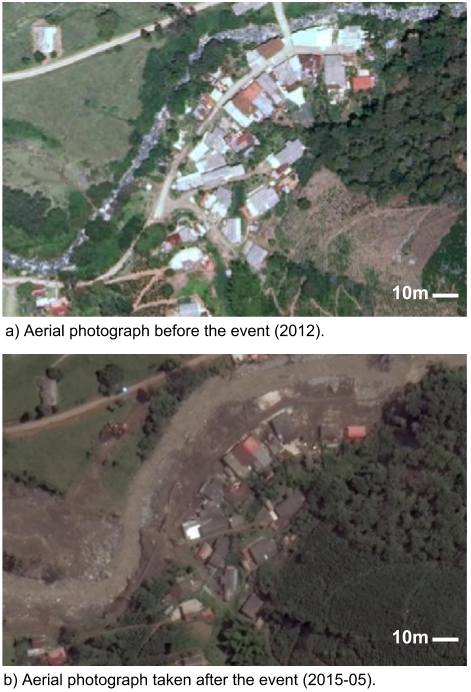
\includegraphics[width=8.3cm]{Figures/Salgar_Before_After.png}
    \caption{Example of infrastructure damage as a result of the La Liboriana \DIFdelbeginFL \DIFdelFL{May 18 of 2015 }\DIFdelendFL flash flood event \DIFdelbeginFL \DIFdelFL{. }\DIFdelendFL \DIFaddbeginFL \DIFaddFL{on May 18, 2015. }\DIFaddendFL a) Aerial photograph before the event (2012) taken during a mission of the Department of Antioquia\DIFdelbeginFL \DIFdelFL{´}\DIFdelendFL \DIFaddbeginFL \DIFaddFL{'}\DIFaddendFL s Government, and b) satellite image after the event (2015-05). The images show the destruction of most houses in that particular community, a bridge over La Liboriana, and the main road. \DIFaddbeginFL \DIFaddFL{All of the houses shown in the 2015 image had to be either demolished or structurally repaired. }\DIFaddendFL The images also present changes in the delineation of the main channel as well as considerable erosion in the river margins.}
    \label{fig:Antes_y_Despues}
\end{figure}

La Liboriana basin \DIFdelbegin \DIFdel{flash flood }\DIFdelend is a typical case of \DIFdelbegin \DIFdel{prediction in ungauged basins  }\DIFdelend \DIFaddbegin \DIFadd{an ungauged basin  }\DIFaddend \citep{Sivapalan2013, Seibert2009, Beven2007, Bonell2006, Yamanaka2017}\DIFdelbegin \DIFdel{.  In this case, there are no local }\DIFdelend \DIFaddbegin \DIFadd{, with non-existing detailed }\DIFaddend records of soils or land use\DIFdelbegin \DIFdel{and the local }\DIFdelend \DIFaddbegin \DIFadd{, topographic maps or digital elevation models (DEMs), and scarce }\DIFaddend hydro-meteorological data\DIFdelbegin \DIFdel{is scarce or non-existent and }\DIFdelend \DIFaddbegin \DIFadd{, }\DIFaddend certainly not available in real time. \DIFdelbegin \DIFdel{Due to the lack of data, La Liboriana case imposes a challenge for flash flood prediction and modeling. }\DIFdelend According to \citet{blschl2012}, there are three methods for using models in these cases. The first strategy is to obtain the required model parameters from \DIFaddbegin \DIFadd{the }\DIFaddend historical basin behavior and the morphological characteristics of the basin. This strategy often leads to low model performance \citep{Duan2006}. The second approach is to inherit the hydrological calibration from a gauged neighboring watershed, which in this case does not exist. The third method is to parameterize the model based on proxy variables, such as hydraulic information obtained during field visits. In the case of the 2015 La Liboriana basin flash flood, there are no previous historical streamflow records \DIFdelbegin \DIFdel{, nor }\DIFdelend \DIFaddbegin \DIFadd{or }\DIFaddend records from a neighboring watershed\DIFdelbegin \DIFdel{, thus}\DIFdelend \DIFaddbegin \DIFadd{; thus, }\DIFaddend we followed the third approach. In this work, we use precipitation information derived from radar, satellite and \DIFdelbegin \DIFdel{aereal images, and }\DIFdelend \DIFaddbegin \DIFadd{aerial images, in addition to }\DIFaddend post-event field visits\DIFaddbegin \DIFadd{, }\DIFaddend to reconstruct the Salgar flash flood event. This study addresses two broad hydrological issues. The first issue consists \DIFdelbegin \DIFdel{in }\DIFdelend \DIFaddbegin \DIFadd{of }\DIFaddend exploring the relationship between rainfall \DIFdelbegin \DIFdel{spatio-temporal }\DIFdelend \DIFaddbegin \DIFadd{spatiotemporal }\DIFaddend structure \citep{Llasat2016,Fragoso2012}, soil moisture and runoff generation \citep{Penna2011,Tramblay2012b,Garambois2013} during the successive rainfall events, and the second issue in proposing a simplified hydrologic modeling scheme\DIFdelbegin \DIFdel{including land-slide and hydraulic sub-models }\DIFdelend \DIFaddbegin \DIFadd{, including landslide and hydraulic submodels }\DIFaddend to assess the potential occurrence of flash flood events.\\

The methodology followed in this study \DIFdelbegin \DIFdel{makes use of a conceptual modeling framework that includes a hydrologic }\DIFdelend \DIFaddbegin \DIFadd{includes a hydrological }\DIFaddend model \citep{Velez2001, Frances2007b}, a shallow \DIFdelbegin \DIFdel{land-slide sub-model \mbox{%DIFAUXCMD
\citep{Aristizabal2016}}\hspace{0pt}%DIFAUXCMD
, and a hydraulic sub-model }\DIFdelend \DIFaddbegin \DIFadd{landslide model and a flash flood model. The landslide submodel follows the formulation described in \mbox{%DIFAUXCMD
\citep{Aristizabal2016}}\hspace{0pt}%DIFAUXCMD
. The hydraulic submodel corresponds to a low-cost 1D model }\DIFaddend (hereafter referred to as HydroFlash) \DIFaddbegin \DIFadd{that }[\DIFadd{assumes infinite sediment supply and}] \DIFadd{estimates the cross-sectional filled area at all time steps}\DIFaddend . The hydrologic model includes virtual tracers to \DIFdelbegin \DIFdel{explore separately }\DIFdelend \DIFaddbegin \DIFadd{separately explore }\DIFaddend the role of runoff and subsurface flow, as well as the relative importance of convective and stratiform precipitation in flash flood generation. The assessment of the interactions between runoff, subsurface flow, and convective-stratiform rainfall allows a better understanding of the short-term hydrological mechanisms leading to the flash flood event.  A comparison between the results from both \DIFdelbegin \DIFdel{sub-models }\DIFdelend \DIFaddbegin \DIFadd{submodels }\DIFaddend and the observed \DIFdelbegin \DIFdel{landslides }\DIFdelend \DIFaddbegin \DIFadd{landslide }\DIFaddend scars and flooded spots helps to evaluate the overall skill of the proposed methodology. \\

The document is structured as follows. Section \ref{sec:data} describes in more detail the region of study, La Liboriana basin, including geomorphological and climatological characteristics of the basin as well as the information sources used in this study. Section \ref{sec:methods} presents a description of the overall methodology and the model used for the reconstruction of the 2015 La Liboriana flash flood event, including flow separation, shallow landslide parameterization, and the proposed \DIFdelbegin \DIFdel{hydraulic model }\DIFdelend \DIFaddbegin \DIFadd{model HydroFlash}\DIFaddend . Section \ref{sec:results} describes the main results of the study, including model validation and sensitivity analysis, and presents results from the \DIFdelbegin \DIFdel{land-slide and inundation sub-models}\DIFdelend \DIFaddbegin \DIFadd{landslide and HydroFlash submodels}\DIFaddend . Section \ref{sec:discussion} includes a discussion on the role of the rainfall structure in the flash flood reconstruction.  Finally, the conclusions are presented in section \ref{sec:conclusions}.


\section{Study \DIFdelbegin \DIFdel{Site }\DIFdelend \DIFaddbegin \DIFadd{site }\DIFaddend and \DIFdelbegin \DIFdel{Data}\DIFdelend \DIFaddbegin \DIFadd{data}\DIFaddend }
\label{sec:data}

\subsection{Catchment description}

The urban area of Salgar municipality is located near the outlet of La Liboriana basin, a small (56 km$^2$) tropical watershed located in the westernmost range of Colombia's Andes (Figure \ref{fig:Ubicacion}). By 2015, the population of Salgar was estimated at \DIFdelbegin \DIFdel{17400 persons, 8800 }\DIFdelend \DIFaddbegin \DIFadd{17,400 persons, 8,800 }\DIFaddend residing in the urban area. La Liboriana basin joins \DIFaddbegin \DIFadd{the }\DIFaddend El Barroso river basin\DIFaddbegin \DIFadd{, }\DIFaddend and both drain to Cauca \DIFdelbegin \DIFdel{river}\DIFdelend \DIFaddbegin \DIFadd{River}\DIFaddend . \\

The availability of the ALOS-PALSAR \DIFdelbegin \DIFdel{Digital Elevation Model (DEM ) }\DIFdelend \DIFaddbegin \DIFadd{DEM }\DIFaddend \citep{ALOS}, with a resolution of \DIFdelbegin \DIFdel{about }\DIFdelend \DIFaddbegin \DIFadd{approximately }\DIFaddend 12.7 m, allows estimating the fundamental geomorphological features of the basin. \DIFaddbegin \DIFadd{While the resolution of the DEM is far from ideal given the scale of the basin and the main channel, it corresponds to the highest spatial resolution freely available for the region.
Additionally, to accomplish the goal of this study, we is to develop and to test a methodology applicable for this type of regions, with scarce information. This is mentioned in a few places in the document, and it has been stressed even more in the current version. }\DIFaddend The average slope of La Liboriana is 57.6\%, and the basin longitude and perimeter are 13.5 $\text{km}$ and 57.8 $\text{km}$, respectively.  The Strahler-Horton order of the main stream is 5, and its longitude and slope are 18.1 $\text{km}$ and 8.1\%, respectively. The highest elevation of the watershed (Cerro Plateado) reaches \DIFdelbegin \DIFdel{3609 }\DIFdelend \DIFaddbegin \DIFadd{3,609 }\DIFaddend meters above sea level (m.a.s.l), while the outlet of the basin is at \DIFdelbegin \DIFdel{1316 }\DIFdelend \DIFaddbegin \DIFadd{1,316 }\DIFaddend m.a.s.l. \DIFdelbegin \DIFdel{.  }\DIFdelend The 99th slope percentile of order 1 streams is 78\%. For streams \DIFaddbegin \DIFadd{of }\DIFaddend order 2, 3, 4, and 5, the 99th slope \DIFdelbegin \DIFdel{percentile }\DIFdelend \DIFaddbegin \DIFadd{percentiles }\DIFaddend are 61, 27, 18 \DIFdelbegin \DIFdel{y }\DIFdelend \DIFaddbegin \DIFadd{and }\DIFaddend 11\%, respectively. Figure \ref{fig:Ubicacion} shows the spatial distribution of the slopes in the watershed. These features are typical of Andean mountainous basins. Geomorphologically, this kind of watershed tends to be prone to the occurrence of flash floods \citep{Lehmann2012, Penna2011, Martin2018,Longoni2016, Ozturk2018, Khosravi2018, Marchi2016, Bisht2018}.\\

%The longitudinal profile (see Figure \ref{fig:Perfil}) exhibits considerable steepness in the upper basin.
%The hypsometric curve shows considerable elevation changes for a cumulative area below 33\%   (see blue line in Figure \ref{fig:Perfil}).  

At the \DIFdelbegin \DIFdel{sub-basin }\DIFdelend \DIFaddbegin \DIFadd{subbasin }\DIFaddend scale, La Liboriana exhibits a vast range of slopes and altitude differences. Figure \ref{fig:Ubicacion} shows the \DIFdelbegin \DIFdel{Height Above the Nearest Drainage -HAND- }\DIFdelend \DIFaddbegin \DIFadd{height above the nearest drainage -"HAND"- }\DIFaddend model   \citep{Renno2008} for La Liboriana. The \DIFdelbegin \DIFdel{HAND }\DIFdelend \DIFaddbegin \DIFadd{"HAND" }\DIFaddend calculates the relative difference between cell $i$ and its nearest streamflow cell $j$. La Liboriana \DIFdelbegin \DIFdel{HAND }\DIFdelend \DIFaddbegin \DIFadd{"HAND" }\DIFaddend exhibits values between 500 and 800 $\text{m}$. Near the outlet of the basin, over the banks, there are values close to 0 m. High HAND values at the upper region of the watershed often denote areas of high potential energy, with increased sediment production and frequent shallow landslide occurrence. Banks with low \DIFdelbegin \DIFdel{HAND }\DIFdelend \DIFaddbegin \DIFadd{"HAND" }\DIFaddend values are more susceptible to flooding and tend to correspond to areas prone to extensive damages caused by extreme events. While the elevation differences described in Figure \ref{fig:Ubicacion} are typical of the region, the social challenges lie in the high vulnerability of Salgar\DIFaddbegin \DIFadd{, }\DIFaddend given the location of the main urban settlement.\\ 

\begin{figure}[t]
\centering
    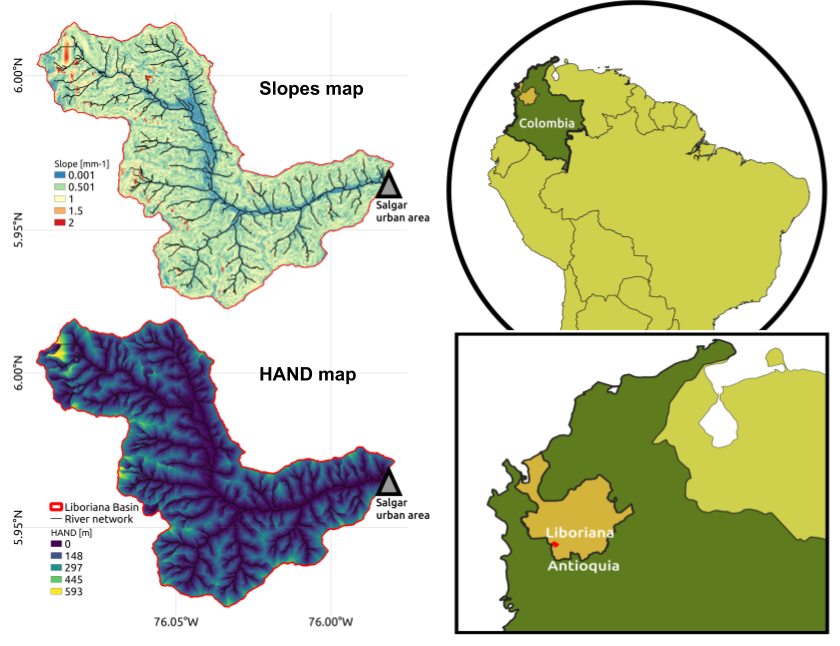
\includegraphics[width=12cm]{Figures/UbicacionV2.png}
    \caption{Geographical context of Liboriana basin, located in Colombia, in the Department of Antioquia. The \DIFdelbeginFL \DIFdelFL{color bar represents }\DIFdelendFL \DIFaddbeginFL \DIFaddFL{panels include }\DIFaddendFL the \DIFdelbeginFL \DIFdelFL{Height Above }\DIFdelendFL \DIFaddbeginFL \DIFaddFL{map of }\DIFaddendFL the \DIFdelbeginFL \DIFdelFL{Nearest Drainage }\DIFdelendFL \DIFaddbeginFL \DIFaddFL{slopes,  the height above the nearest drainage }\DIFaddendFL (\DIFaddbeginFL \DIFaddFL{"}\DIFaddendFL HAND\DIFaddbeginFL \DIFaddFL{"}\DIFaddendFL )\DIFaddbeginFL \DIFaddFL{, and the soil type map}\DIFaddendFL . \DIFaddbeginFL \DIFaddFL{The "}\DIFaddendFL HAND\DIFaddbeginFL \DIFaddFL{" }\DIFaddendFL values where estimated using the same resolution of the DEM (12.7 $\text{m}$).  Low \DIFaddbeginFL \DIFaddFL{"}\DIFaddendFL HAND\DIFaddbeginFL \DIFaddFL{" }\DIFaddendFL values correspond to areas prone to flooding. \DIFaddbeginFL \DIFaddFL{Note that the soil type map is an extrapolation of the soil properties based on the slope.}\DIFaddendFL }
    \label{fig:Ubicacion}
\end{figure}


%\begin{figure}[t]
%\centering
 %   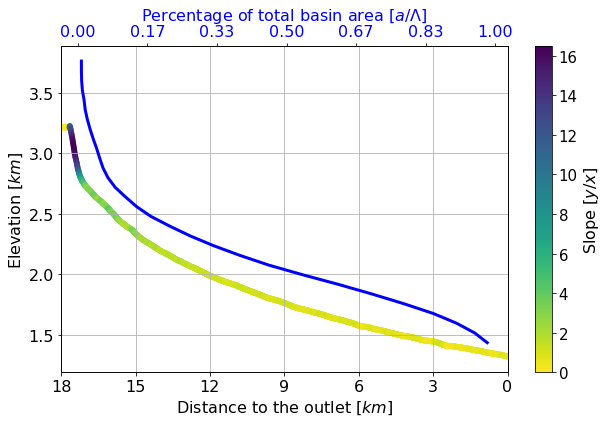
\includegraphics[width=8.3cm]{Figures/Perfil_Cauce.png}
 %   \caption{Longitudinal profile of the principal stream (colored line) from the upper part of the basin to its outlet at the entrance of the urban area, hypsometric curve of the drainage basin (blue line).}
 %   \label{fig:Perfil}
%\end{figure}

Vegetation and land use vary considerably within the basin. Figure \ref{fig:landuse} shows land use in different regions of the watershed from a 2012 \DIFdelbegin \DIFdel{aereal }\DIFdelend \DIFaddbegin \DIFadd{aerial }\DIFaddend image. In the upper La Liboriana basin, there is dense vegetation (see Zoom 1 in Figure \ref{fig:landuse}), with a high percentage of \DIFdelbegin \DIFdel{tropical forests, with }\DIFdelend \DIFaddbegin \DIFadd{the area covered by tropical forests and }\DIFaddend the presence of grass and few crop fields.  A portion of the upper watershed is considered a national park. Hillslopes near the divide do not evidence significant anthropic intervention most likely due steepness of this region. Down the hills and at the bottom of the valley there are coffee plantations (the primary economic activity of the region) and pastures. Downstream (Figure \ref{fig:landuse}, Zoom 2), \DIFdelbegin \DIFdel{it is evident }\DIFdelend the presence of crops \DIFaddbegin \DIFadd{is evident }\DIFaddend among forest and grass \DIFaddbegin \DIFadd{areas}\DIFaddend . Near the middle of the basin (Figure \ref{fig:landuse}, Zoom 3), the presence of crops is more \DIFdelbegin \DIFdel{notorious }\DIFdelend \DIFaddbegin \DIFadd{obvious, }\DIFaddend and human settlements and roads start to appear. The watershed exhibits grazing areas and urban development near the river banks. In Figure \ref{fig:landuse}, Zoom 4, corresponding to the first affected urban area from upstream to downstream during the flash flood, it is also possible to see a marked presence of crops and some forest patches. Finally, \DIFdelbegin \DIFdel{zoom }\DIFdelend \DIFaddbegin \DIFadd{Zoom }\DIFaddend 5 shows the main urban area of Salgar surrounded by crops, grass and an important loss of forest coverage. \\

\begin{figure}[t]
\centering
\includegraphics[width=12cm]{Salgar_VegetationDetails.png}
\caption{Land use in different regions of La Liboriana watershed from a 2012 \DIFdelbeginFL \DIFdelFL{aereal images }\DIFdelendFL \DIFaddbeginFL \DIFaddFL{aerial image }\DIFaddendFL (Source: Department of Antioquia.\DIFaddbeginFL \DIFaddFL{)}\DIFaddendFL }
\label{fig:landuse}
\end{figure}


One of the challenges for hydrological modeling and risk management in the country is that soils are not well mapped; the national soil cartography is usually available in a 1:\DIFdelbegin \DIFdel{400.000 }\DIFdelend \DIFaddbegin \DIFadd{400,000 }\DIFaddend scale. At this scale, the municipality of Salgar, including La Liboriana basin,  corresponds to only one category of soil texture. \citet{Osorio2008}, based on field campaign observations and laboratory tests, described La Liboriana soils as a well-drained soil with poor retention capacity. Organic material is predominant in the first layer\DIFaddbegin \DIFadd{, }\DIFaddend and clay loam soil \DIFaddbegin \DIFadd{predominates }\DIFaddend within the second \DIFdelbegin \DIFdel{one}\DIFdelend \DIFaddbegin \DIFadd{layer}\DIFaddend . The depth of the soil is hillslope dependent, varying from 20 $cm$ to 1 $m$ \citep{Osorio2008}. Table \ref{tab:suelos} provides a summary of soil characteristics for five different categories, all as a function of slope. Each soil category has a corresponding depth and a qualitative description of permeability and retention.\\

\begin{table}[t]
  \caption{Description of the soils in the region \citep{Osorio2008}.}
  \DIFdelbeginFL %DIFDELCMD < \begin{tabular}{lcccr}
%DIFDELCMD <   %%%
\DIFdelendFL \DIFaddbeginFL \begin{tabular}{lccccr}
  \DIFaddendFL \hline
    \textbf{Type} & \textbf{Slope} & \textbf{Depth [$m$]} & \textbf{Retention} & \textbf{Permeability} \DIFaddbeginFL & \textbf{\DIFaddFL{Percentage}} \DIFaddendFL \\    
  \hline
    \textbf{Class III} & \DIFdelbeginFL \DIFdelFL{12-25 }\DIFdelendFL \DIFaddbeginFL \DIFaddFL{<12 }\DIFaddendFL & 0.6 & \DIFdelbeginFL \DIFdelFL{Mean }\DIFdelendFL \DIFaddbeginFL \DIFaddFL{Low }\DIFaddendFL & \DIFdelbeginFL \DIFdelFL{Mean }\DIFdelendFL \DIFaddbeginFL \DIFaddFL{High }&  \DIFaddFL{3.2}\DIFaddendFL \\
    \textbf{Class IV} & \DIFdelbeginFL \DIFdelFL{<12 }\DIFdelendFL \DIFaddbeginFL \DIFaddFL{12-25 }\DIFaddendFL & 0.6 & \DIFdelbeginFL \DIFdelFL{Low }\DIFdelendFL \DIFaddbeginFL \DIFaddFL{Mean }\DIFaddendFL & \DIFdelbeginFL \DIFdelFL{High }\DIFdelendFL \DIFaddbeginFL \DIFaddFL{Mean }& \DIFaddFL{8.3}\DIFaddendFL \\
    \textbf{Class VI} & 25-30 & 1.0 & Mean & Mean \DIFaddbeginFL & \DIFaddFL{2.1}\DIFaddendFL \\
    \textbf{Class VII} & 30-50 & 0.3 & Too Low & \DIFdelbeginFL \DIFdelFL{Slow }\DIFdelendFL \DIFaddbeginFL \DIFaddFL{Low }& \DIFaddFL{25.5}\DIFaddendFL \\
    \textbf{Class VIII} & >50 & 0.2 & Too Low & \DIFdelbeginFL \DIFdelFL{Slow }\DIFdelendFL \DIFaddbeginFL \DIFaddFL{Low }& \DIFaddFL{60.0}\DIFaddendFL \\
  \hline
  \end{tabular}
%   \belowtable{The description given by the IGAC institute is subjective, without mentioning exact values of retention and permeability.  The depth values given are approximations.} % Table Footnotes
  \label{tab:suelos}
\end{table}

\subsection{Flash flood post-event observations}

We conducted a field campaign a few days after the May 18th flash flood event to assess \DIFaddbegin \DIFadd{the }\DIFaddend cross-section geometry along the main channel in different sites, including at the outlet of the basin. \DIFdelbegin \DIFdel{Unfortunately, most of the affected areas were not accessible after the event and it was not  possible to obtain reliable information in other locations along the main channel other than at the outlet of the basin. }\DIFdelend During the campaign, we measured sectional distances and \DIFdelbegin \DIFdel{surface water speeds }\DIFdelend \DIFaddbegin \DIFadd{the surface water speed at the time of the visit, }\DIFaddend at different points of the streamflow. \DIFaddbegin \DIFadd{The surface water speed was measured using a hand-held Stalker Pro II surface velocity radar. }\DIFaddend We also identified traditional post-event terrain, \DIFdelbegin \DIFdel{land-cover}\DIFdelend \DIFaddbegin \DIFadd{land cover}\DIFaddend , vegetation and infrastructure markers to assess the high-water marks associated with the peak of the flash flood.  Figure \ref{fig:Seccion} presents the selected cross-section used for the estimation of the maximum discharge during the flash flood given its geometrical and hydraulic regularity. The section has a rectangular shape, 4.6 $\text{m}$ wide and a height of 5 $\text{m}$ for a total area of \DIFdelbegin \DIFdel{about }\DIFdelend \DIFaddbegin \DIFadd{approximately }\DIFaddend 23 $\text{m}^2$. A visual inspection of the flooded house around the section, located 4-5 $\text{m}$ away from the channel, reveals the presence of mud marks on the walls with heights varying between 0.5 and 1.2 $\text{m}$ (see Figure \ref{fig:Seccion}). The area of the section plus the flooded area during the event was estimated to be approximately 37 $\text{m}^2$.  During the campaign\DIFaddbegin \DIFadd{, }\DIFaddend we measured surface speeds in the channel oscillating between 2 and 3 $\text{ms}^{-1}$\DIFaddbegin \DIFadd{, for a  3 m$^3 \text{s}^{-1}$ discharge}\DIFaddend . In instrumented basins in the region, with similar characteristics in terms of area and slopes, we have recorded peak flow surface water speeds oscillating between 5 and 7 $\text{ms}^{-1}$ \DIFaddbegin \DIFadd{(See Figure \ref{fig:Appendix})}\DIFaddend . By assuming an area of 37 $\text{m}^2$ and \DIFdelbegin \DIFdel{the mentioned surface speeds}\DIFdelend \DIFaddbegin \DIFadd{velocities between 5 and 6}\DIFaddend ,  we estimate that the observed flash flood peak flow may have been between 185 and 222 $\text{m}^3\text{s}^{-1}$. \DIFdelbegin \DIFdel{The timing of the peak flow is also important information. }\DIFdelend Local authorities reported that the peak streamflow reached the urban perimeter after 2:10 a.m. on May 18th \DIFaddbegin \DIFadd{(personal communication during the field visit)}\DIFaddend . Some reports state that the peak flow in the most affected community occurred \DIFdelbegin \DIFdel{around }\DIFdelend \DIFaddbegin \DIFadd{at approximately }\DIFaddend 2:40 a.m \DIFaddbegin \footnote{\DIFadd{As reported by the media and the national government: }\url{http://www.elcolombiano.com/antioquia/tragedia-en-antioquia-salgar-un-ano-despues-XX4145514}\DIFadd{, }\url{https://caracol.com.co/emisora/2015/12/25/medellin/1451076926_792470.html}\DIFadd{, }\url{http://portal.gestiondelriesgo.gov.co/Paginas/Noticias/2015/Antecion-Emergencia-Salgar-Antioquia.aspx}}\DIFaddend .\\

There is also relevant aerial information before and after the occurrence of the event.  During 2012, the Department of Antioquia conducted a detailed aerial survey of the Salgar municipality, and \DIFaddbegin \DIFadd{a }\DIFaddend few days after the event\DIFdelbegin \DIFdel{Google displayed publically high }\DIFdelend \DIFaddbegin \DIFadd{, DigitalGlobe and CNES/Airbus made available highly }\DIFaddend detailed satellite images of the same region. \DIFdelbegin \DIFdel{The }\DIFdelend \DIFaddbegin \DIFadd{We empirically performed a detailed }\DIFaddend contrast between both products \DIFdelbegin \DIFdel{provides }\DIFdelend \DIFaddbegin \DIFadd{by using a geographic information system (QGIS), which provided us with }\DIFaddend information about flooded areas and landslide locations \DIFaddbegin \DIFadd{(see Figures \ref{fig:Antes_y_Despues} and \ref{fig:SimFloodSpots})}\DIFaddend . Field campaign estimates and aerial imagery are central to validate the results obtained from the proposed models.\\

\begin{figure}[t]
\centering
    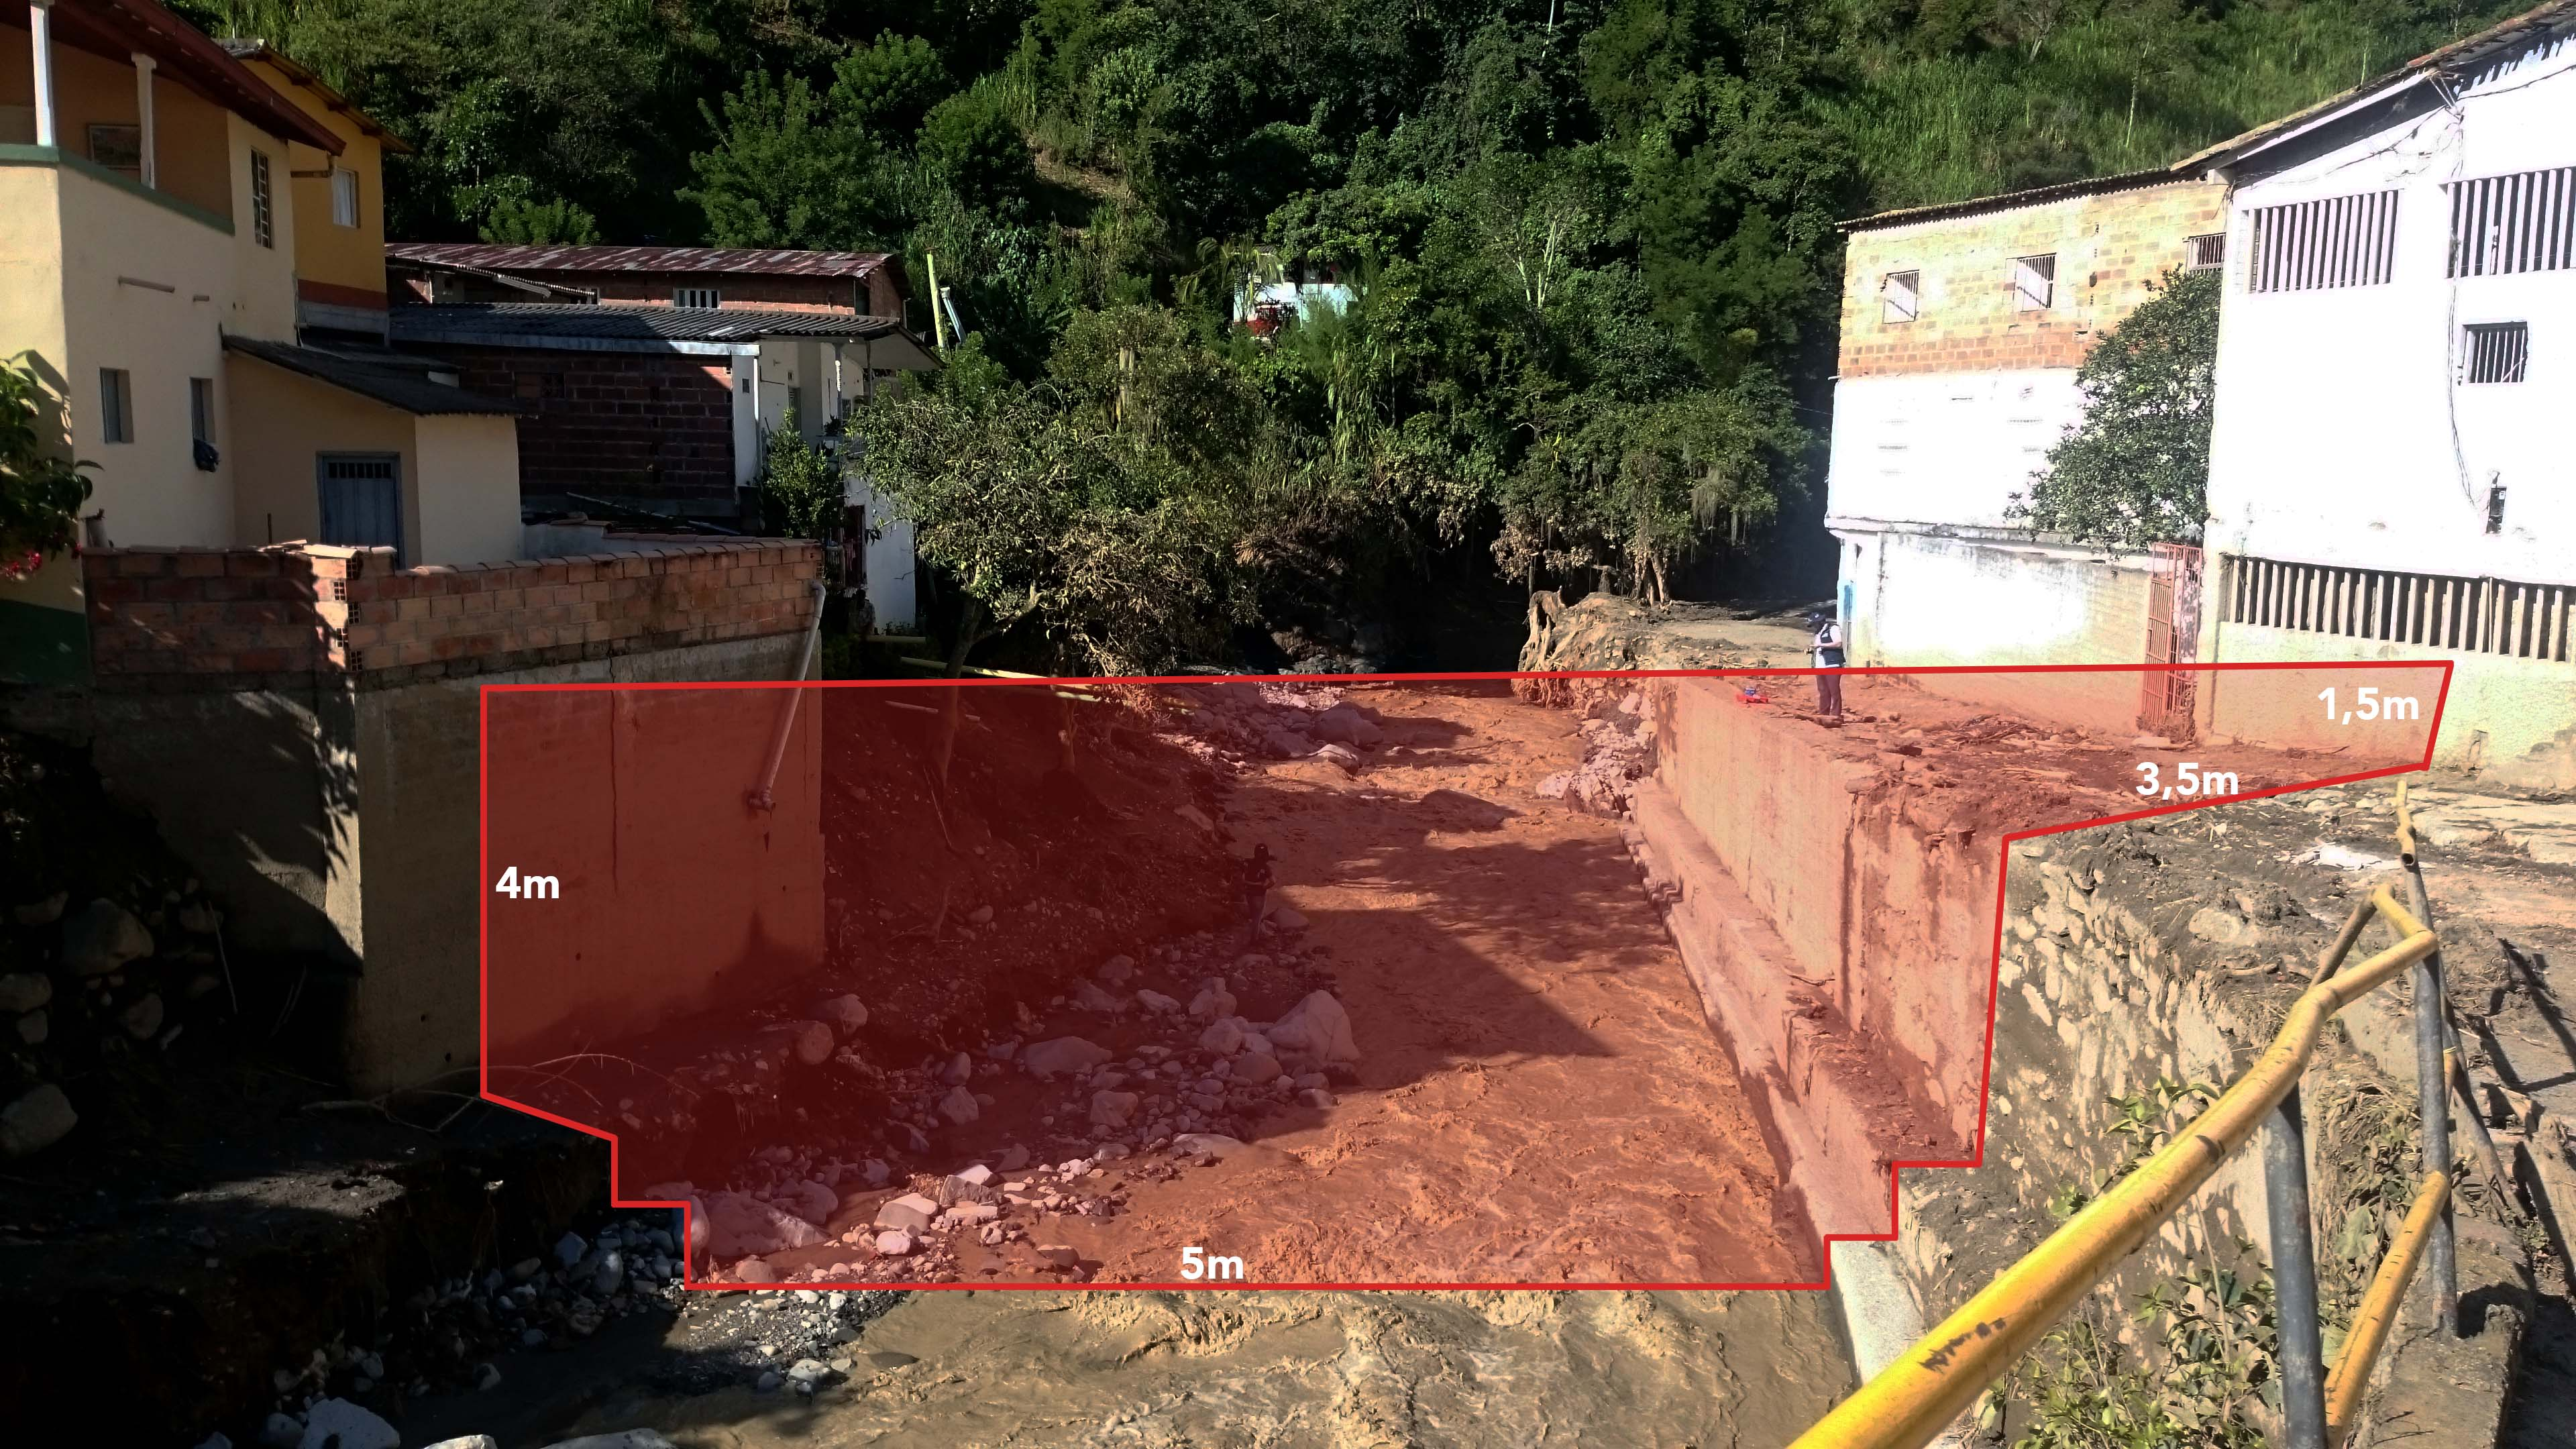
\includegraphics[width=8.3cm]{Figures/Salgar_SeccionAguasAbajo.jpg}
    \caption{Channel cross-section \DIFdelbeginFL \DIFdelFL{shown }\DIFdelendFL \DIFaddbeginFL \DIFaddFL{showing }\DIFaddendFL an example of flooded infrastructure after the flash flood event. The section shows mud marks on the walls with heights varying between 0.5 and 1.2 m. These mud stains are evident in buildings located 4-5 m away from the channel. The photograph also shows the width of the channel and the total estimated depth during the flash flood. \DIFaddbeginFL \DIFaddFL{The cross-section is located downstream the bridge shown in the picture.}\DIFaddendFL }
    \label{fig:Seccion}
\end{figure}

\subsection{Rainfall \DIFdelbegin \DIFdel{Information}\DIFdelend \DIFaddbegin \DIFadd{information}\DIFaddend }

The assessment of the 2015 Salgar flash flood event following a hydrological modeling strategy uses a radar-based QPE technique developed by Sepúlveda and Hoyos (2019) using rainfall gauges and disdrometers within the radar domain to obtain spatiotemporal precipitation maps over the basin. A detailed description of the rainfall estimation, as well as the overall meteorological conditions that led to the La Liboriana extreme event, are described in a companion paper (\DIFdelbegin \DIFdel{Hoyos et al. 2019}\DIFdelend \DIFaddbegin \DIFadd{\mbox{%DIFAUXCMD
\citet{Hoyos2019}}\hspace{0pt}%DIFAUXCMD
}\DIFaddend ). The QPE technique uses retrievals from a C-band polarimetric Doppler weather radar operated by the Sistema de Alerta Temprana de Medellín y el Valle de Aburra (SIATA, a local early warning system from a neighboring region, www.siata.gov.co), located \DIFdelbegin \DIFdel{around }\DIFdelend \DIFaddbegin \DIFadd{approximately }\DIFaddend 90 $\text{km}$ away from the basin. The radar has an optimal \DIFdelbegin \DIFdel{optimum range }\DIFdelend \DIFaddbegin \DIFadd{range in a radius }\DIFaddend of 120 $\text{km}$ \DIFdelbegin \DIFdel{radius }\DIFdelend for rainfall estimation and a maximum operational range of 240 $\text{km}$ for weather detection. The radar operating strategy allows obtaining precipitation information every 5 minutes\DIFaddbegin \DIFadd{, }\DIFaddend with a spatial resolution \DIFdelbegin \DIFdel{is about }\DIFdelend \DIFaddbegin \DIFadd{of approximately }\DIFaddend 128 $\text{m}$. The results of the radar QPE methodology indicate that the rainfall estimation works well within a radius of \DIFdelbegin \DIFdel{120km}\DIFdelend \DIFaddbegin \DIFadd{120 km}\DIFaddend . Despite the distance between the radar and the basin, and the mountains between them, there are no blind spots for the radar. A comparison between the radar QPE estimates and records from two rain gauges installed three days after the flash flood event show a correlation for an hourly time scale of 0.65. In addition to the rainfall quantification, radar retrievals, before feeding the hydrologic model, are classified in convective and stratiform areas following a methodology proposed by \DIFdelbegin \DIFdel{\mbox{%DIFAUXCMD
\citet{Houze2015} }\hspace{0pt}%DIFAUXCMD
and \mbox{%DIFAUXCMD
\citet{Steiner1995}}\hspace{0pt}%DIFAUXCMD
}\DIFdelend \DIFaddbegin \DIFadd{\mbox{%DIFAUXCMD
\citet{Yuter1997} }\hspace{0pt}%DIFAUXCMD
and \mbox{%DIFAUXCMD
\citet{Steiner1995}}\hspace{0pt}%DIFAUXCMD
, based on the intensity and sharpness of the reflectivity peaks. The methodology has been widely used in tropical regions as reported in the review by \mbox{%DIFAUXCMD
\citet{Houze2015}}\hspace{0pt}%DIFAUXCMD
}\DIFaddend .\\


Between May \DIFdelbegin \DIFdel{15th and May 18th}\DIFdelend \DIFaddbegin \DIFadd{15 and May 18}\DIFaddend , 2015, several storms took place over La Liboriana basin.  During the night of May \DIFdelbegin \DIFdel{17th}\DIFdelend \DIFaddbegin \DIFadd{17}\DIFaddend , between 02:00 and 09:00 a.m. (local time), a precipitation event covered \DIFdelbegin \DIFdel{almost all }\DIFdelend \DIFaddbegin \DIFadd{in almost all of }\DIFaddend the basin (hereafter referred to as precipitation Event 1). Twenty hours later, between 23:00 p.m. \DIFdelbegin \DIFdel{of }\DIFdelend \DIFaddbegin \DIFadd{on }\DIFaddend May 17 and 02:00 a.m. \DIFdelbegin \DIFdel{of }\DIFdelend \DIFaddbegin \DIFadd{on }\DIFaddend May 18\DIFaddbegin \DIFadd{, }\DIFaddend two successive extreme convective systems occurred over the basin with the maximum intensity in the upper hills (precipitation Event 2). Event 1 corresponds mainly to a stratiform event \DIFdelbegin \DIFdel{, covering almost all }\DIFdelend \DIFaddbegin \DIFadd{that covered almost all of }\DIFaddend the basin area and \DIFdelbegin \DIFdel{with }\DIFdelend \DIFaddbegin \DIFadd{incurred }\DIFaddend an average precipitation accumulation of 47 $\text{mm}$. Event 2 accumulated, \DIFdelbegin \DIFdel{in }\DIFdelend \DIFaddbegin \DIFadd{on }\DIFaddend average over the basin, \DIFdelbegin \DIFdel{around }\DIFdelend \DIFaddbegin \DIFadd{approximately }\DIFaddend 38 $\text{mm}$\DIFdelbegin \DIFdel{, however}\DIFdelend \DIFaddbegin \DIFadd{; however, }\DIFaddend over the upper watershed\DIFaddbegin \DIFadd{, }\DIFaddend the accumulation exceeded 180 $\text{mm}$ \DIFaddbegin \DIFadd{according to the estimated rainfall amounts based on the radar measurements. \mbox{%DIFAUXCMD
\citet{Hoyos2019} }\hspace{0pt}%DIFAUXCMD
show that the individual events duringh May 2015 were not exceptional, the climatological anomalies were negative-to-normal, and the synoptic patterns around the extreme event were similar to the expected ones for the region, but the combination of high rainfall accumulation in a 96-hour period as a result of successive precipitation events over the basin, followed by a moderate extreme event during May 18, is unique in the available observational radar record, in particular for the upper part of the basin}\DIFaddend . Figure \ref{fig:separacionLluvia}a presents the temporal evolution of the \DIFaddbegin \DIFadd{estimated }\DIFaddend convective-stratiform rainfall partitioning during both Events 1 and 2. The main difference between both events is the timing of the convective versus stratiform participation within each case. Event 1 started as a stratiform precipitation event moving from the southwest, from the Department of Chocó to the Department of Antioquia across \DIFdelbegin \DIFdel{westernmost Andes mountain range. Chochó is the rainiest department in Colombia, and one of the wettest places on Earth, due to the inflow of moisture from the Pacific Ocean and the orientation of the }\DIFdelend \DIFaddbegin \DIFadd{the westernmost }\DIFaddend Andes mountain range\DIFdelbegin \DIFdel{\mbox{%DIFAUXCMD
\citep{poveda2000, Mapes2003}}\hspace{0pt}%DIFAUXCMD
}\DIFdelend .  After 3 hours of stratiform rainfall, training convective cores move over La Liboriana basin generating intense precipitation peaks \DIFdelbegin \DIFdel{during }\DIFdelend \DIFaddbegin \DIFadd{over }\DIFaddend 2.5 hours. It is important to note that these cores did not strengthen within La Liboriana basin; these systems formed and intensified over the western hills of Farallones de Citará\DIFaddbegin \DIFadd{, }\DIFaddend draining to the Department of Chocó towards the Atrato river. The latter is not a minor fact because once the convective system moved with a northeast direction, the maximum intensity cores did not fall over the steepest hills of La Liboriana basin but rather near the basin outlet where the slopes are considerably flatter. Figure \ref{fig:separacionLluvia}b shows the spatial distribution cumulative rainfall during Event 1, with the maximum precipitation located \DIFdelbegin \DIFdel{towards }\DIFdelend \DIFaddbegin \DIFadd{toward }\DIFaddend the bottom third of the basin. Event 2, on the other hand, started as a thunderstorm training event with two convective cores moving from the southeast\DIFdelbegin \DIFdel{followed by }\DIFdelend \DIFaddbegin \DIFadd{, followed by the }\DIFaddend remaining stratiform precipitation. Even though the average cumulative rainfall over the basin was 9 mm less than during Event 1, this event is characterized by orographic intensification within the basin\DIFaddbegin \DIFadd{, }\DIFaddend leading to a more heterogeneous spatial distribution \DIFdelbegin \DIFdel{and }\DIFdelend with the highest cumulative precipitation in the steepest portion of the basin (see Figure \ref{fig:separacionLluvia}b). \DIFdelbegin \DIFdel{Event 2 spatial distribution }\DIFdelend \DIFaddbegin \DIFadd{The spatial distribution of Event 2 }\DIFaddend and highly localized observed intensities most likely led to the flash-flooding episode, as \DIFdelbegin \DIFdel{it is }\DIFdelend explored in this work. \\


\begin{figure}[t]
\centering
 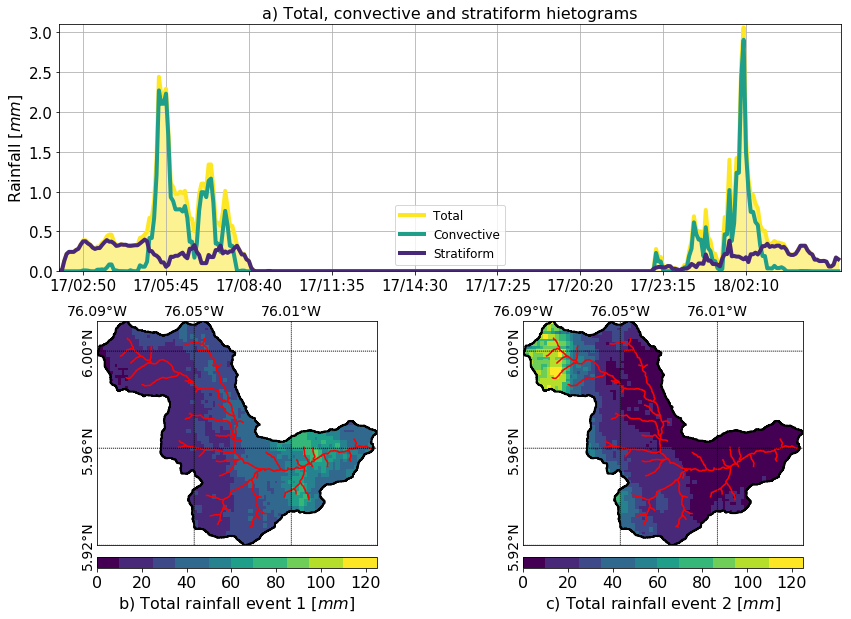
\includegraphics[width=12cm]{Figures/Rainfall_separation.png}
 \caption{a) Temporal evolution of the convective-stratiform rainfall partitioning during both Events 1 and \DIFdelbeginFL \DIFdelFL{2. }\DIFdelendFL \DIFaddbeginFL \DIFaddFL{2 (units in mm per 5 min). }\DIFaddendFL The figure shows the total rainfall (yellow), and the convective (blue) and stratiform (green) portions integrated over La Liboriana basin. b) and c) Spatial distribution of the cumulative rainfall during Events 1 and 2 over La Liboriana basin\DIFaddbeginFL \DIFaddFL{, respectively}\DIFaddendFL .}
    \label{fig:separacionLluvia}
\end{figure}

The data requirements \DIFdelbegin \DIFdel{, }\DIFdelend and rainfall preprocessing needed for the overall methodology followed in the reconstruction of the 2015 Salgar flash flood are summarized in Table \ref{tab:data} and are  presented in a schematic diagram in Figure \ref{fig:EsquemaMetodologico}. \\


    \begin{table}[]
        \centering
        \begin{tabularx}{\textwidth}{p{2.5cm} p{4cm} p{2cm} p{4cm} }
    \hline 
    Item & Description & Period & Usage \\
    \hline
Radar data & QPE rainfall estimations & 2015-05-17 to 2015-05-18 & Hydrologic model runs. Rainfall characterization and event analysis. \\
Field campaign & Maximum streamflow estimation \DIFdelbeginFL \DIFdelFL{trough }\DIFdelendFL \DIFaddbeginFL \DIFaddFL{through }\DIFaddendFL visual inspection & 2015-05-20 & Hydrologic model comparison for indirect validation. \\
Satellite imagery & Visible channel compositions from the \DIFdelbeginFL \DIFdelFL{Digital Globe }\DIFdelendFL \DIFaddbeginFL \DIFaddFL{DigitalGlobe }\DIFaddendFL CNES imagery & 2015-05 (post-event) & Flash flood model validation, shallow \DIFdelbeginFL \DIFdelFL{land-slides }\DIFdelendFL \DIFaddbeginFL \DIFaddFL{landslides }\DIFaddendFL model validation, and comparison with pre-event conditions. \\
Aerial photos & Aerial photos taken by the government of Antioquia during 2012. & 2012 & Pre-event conditions comparison. \\
Soils description & Physical description of the soils of the region by \cite{Osorio2008} & 2008 & Hydrologic model setup. \\
\hline
\end{tabularx}
        \caption{Summary of the data used for the model setup.}
        \label{tab:data}
    \end{table}


\begin{figure}[t]
\centering
 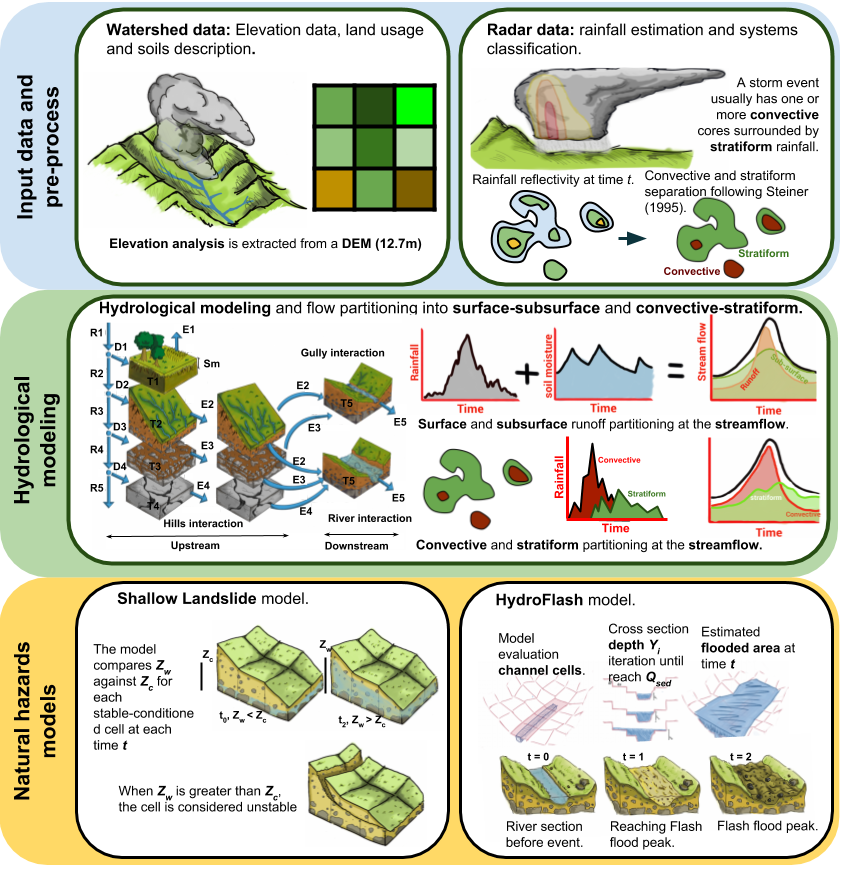
\includegraphics[width=12cm]{Figures/Salgar_Esquema_v2.png}
 \caption{Illustrative diagram of the methodology followed in the present study. The top row represents the availability of a detailed DEM and  radar-based QPE as the basis of the modeling framework. The second row represents the mains aspects of the distributed hydrologic model used. In each cell\DIFaddbeginFL \DIFaddFL{, }\DIFaddendFL five tanks represent the hydrological processes including capillary (tank 1), gravitational (tank 2), runoff (tank 3), baseflow (tank 4) and channel storage (tank 5). The state of each tank varies \DIFdelbeginFL \DIFdelFL{in }\DIFdelendFL \DIFaddbeginFL \DIFaddFL{as a }\DIFaddendFL function of vertical and lateral flows as shown in the diagram, where the storage is represented by $S_i$ \DIFdelbeginFL \DIFdelFL{, }\DIFdelendFL \DIFaddbeginFL \DIFaddFL{and }\DIFaddendFL the vertical input by $D_i$\DIFaddbeginFL \DIFaddFL{, }\DIFaddendFL which in turns depends on the vertical flow through tanks $R_i$. $E_i$ represents the downstream connection between cells \DIFdelbeginFL \DIFdelFL{, }\DIFdelendFL and evaporation. The implementation of convective and stratiform rainfall separation and virtual tracers is also portrayed. The implementation of the shallow landslides model and HydroFlash are schematized in the bottom row.}
    \label{fig:EsquemaMetodologico}
\end{figure}



%%-----------------------------------------------------------
%%-----------------------------------------------------------
%Methodology
%%-----------------------------------------------------------
%%-----------------------------------------------------------
\section{Methodology}
\label{sec:methods}

\subsection{Hydrological modeling framework}

The availability of radar-based QPE and a detailed DEM allows the use of a modeling framework based on the distributed hydrologic model described in \citet{Velez2001} and \citet{Frances2007b} with important modifications. The hydrologic model simulates different hydrological processes as independent, but \DIFaddbegin \DIFadd{with }\DIFaddend interacting storages (second row, left panel in Figure \ref{fig:EsquemaMetodologico}). The model distributes processes by cells \DIFaddbegin \DIFadd{with a spatial resolution of 12.7 m (same as the DEM used)}\DIFaddend ; in each cell, five tanks represent the hydrological processes including capillary (tank 1), gravitational (tank 2), runoff (tank 3), baseflow (tank 4) and channel storage (tank 5). The state of each tank varies \DIFdelbegin \DIFdel{in }\DIFdelend \DIFaddbegin \DIFadd{as a }\DIFaddend function of vertical and lateral flows as shown in the diagram, where the storage is represented by $S_i$ \DIFdelbegin \DIFdel{, }\DIFdelend \DIFaddbegin \DIFadd{and }\DIFaddend the vertical input to each tank by $D_i$, which in turns depends on the vertical flow through tanks $R_i$. $E_i$ represents the downstream connection between cells, except for tank 1, where $E_1$ represents the evaporation rate. Vertical flows are only time dependent, while lateral flows could also depend on the actual state of the tank (kinematic approximation).\\

The model modifications fall in four different categories: (i) the direct use of radar QPE as a source of rainfall information, (ii) the implementation of virtual tracers for surface and subsurface discharge as well as for convective and stratiform water tracing,  (iii) the enforcement of a maximum gravitational storage ($H_{g}$) to allow Hortonian runoff (return flow from $S_3$ (tank 3) to $S_2$ (tank 2)), and (iv) the development of two modules for hazard assessment. The implementation of virtual tracers is represented in the top two right panels of the diagram in Figure \ref{fig:EsquemaMetodologico}.\\

\DIFaddbegin \DIFadd{Additionally, in this study, we propose a graphical method to assess the soil-rainfall-discharge coupling holistically. The first step is to classify all the cells within the watershed in a predetermined number of groups according to their localization and the distance to the outlet. The aim is to establish a coherent and robust spatial discretization, thus allowing the concurrent spatiotemporal variability of the different processes to be summarized in 2D diagrams. Figure \ref{fig:groupsexample} shows the watershed grouping as a function of localization and distance to the outlet for La Liboriana basin using a 20 and a 50-groups categorization.}\\


\begin{figure}[t!]
\centering
 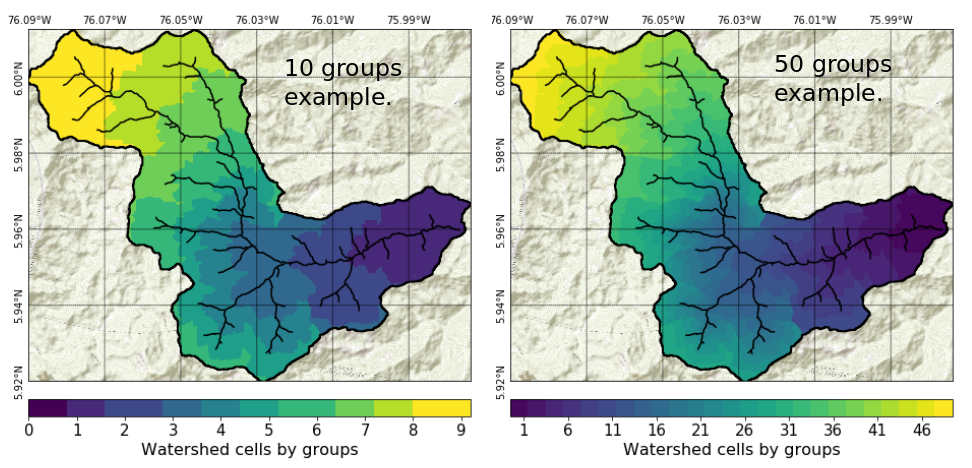
\includegraphics[width=9cm]{Figures/Mapas_Grupos.png}
 \caption{\DIFaddFL{Example of watershed grouping as a function of of their localization and distance to the outlet for La Liboriana basin using a 20 and a 50-groups categorization.}}
    \label{fig:groupsexample}
\end{figure}


\DIFaddend \subsubsection{Hydrological runoff scheme modification}

In the model, horizontal flow equations could be either linear or potential, as shown in equation \ref{eq:generica}. In the modified hydrologic model, $\beta$ and $\alpha$ are estimated by the user and then \DIFdelbegin \DIFdel{set into }\DIFdelend \DIFaddbegin \DIFadd{implemented in }\DIFaddend the model. In the \DIFdelbegin \DIFdel{non-lineal approximation}\DIFdelend \DIFaddbegin \DIFadd{nonlinear approximation, }\DIFaddend $\beta$ is a coefficient that summarizes local properties \DIFaddbegin \DIFadd{that are }\DIFaddend invariant over time, \DIFdelbegin \DIFdel{like }\DIFdelend \DIFaddbegin \DIFadd{such as }\DIFaddend the slope or the hydraulic conductivity. $\alpha$ is an exponent that \DIFdelbegin \DIFdel{change in }\DIFdelend \DIFaddbegin \DIFadd{changes as a }\DIFaddend function of the adopted approximation. From equations \ref{eq:generica} to \ref{eq:kubota}, \DIFdelbegin \DIFdel{$A_i(t)$ }\DIFdelend \DIFaddbegin \DIFadd{$A_i(t) [m^2]$ }\DIFaddend corresponds to the sectional area of each storage, \DIFaddbegin \DIFadd{and }\DIFaddend $A_i(t)$ \DIFdelbegin \DIFdel{vary in }\DIFdelend \DIFaddbegin \DIFadd{varies as a }\DIFaddend function of the tank storage \DIFdelbegin \DIFdel{$S_i(t)$ }\DIFdelend \DIFaddbegin \DIFadd{$S_i(t) [mm]$ }\DIFaddend according to equation \ref{eq:balance}. \DIFaddbegin \DIFadd{Finally, $v_{i}$ corresponds to the estimated velocity in $m/s$.
}\DIFaddend 

\begin{equation}
 v\DIFdelbegin \DIFdel{_{tank}}\DIFdelend \DIFaddbegin \DIFadd{_{i}}\DIFaddend (t) = \beta A_i(t) ^{\alpha} 
    \label{eq:generica}
\end{equation}

\DIFdelbegin \DIFdel{Non-linear }\DIFdelend \DIFaddbegin \DIFadd{Nonlinear }\DIFaddend equations in lateral flows \DIFdelbegin \DIFdel{could }\DIFdelend \DIFaddbegin \DIFadd{can }\DIFaddend result in a better representation of processes at high resolutions \citep{Beven1981, Kirkby1967}.  A \DIFdelbegin \DIFdel{non-linear approximation to }\DIFdelend \DIFaddbegin \DIFadd{nonlinear approximation of }\DIFaddend runoff is presented in equation \ref{eq:runoff}. This approximation is a modification of Manning's formula for flow in gullies. According to \citet{Foster1984}, $\varepsilon$ and $e_1$ are a coefficient and an exponent used to translate the \DIFdelbegin \DIFdel{manning }\DIFdelend \DIFaddbegin \DIFadd{Manning }\DIFaddend channel concept into multiple small channels or gullies. The values of $\varepsilon$ and $e_1$ are 0.5 and 0.64, respectively \citep{Foster1984}. $A_2$ is the corresponding sectional area obtained from $S_2$ by using \DIFdelbegin \DIFdel{the }\DIFdelend equation (\ref{eq:balance}). \DIFdelbegin \DIFdel{And }\DIFdelend \DIFaddbegin \DIFadd{In addition, }\DIFaddend $S_0$ is the slope of the cell.\DIFaddbegin \\     
\DIFaddend 

The \DIFdelbegin \DIFdel{non-linear }\DIFdelend \DIFaddbegin \DIFadd{nonlinear }\DIFaddend equation \ref{eq:kubota} corresponds to an adaptation of \DIFaddbegin \DIFadd{the }\DIFaddend \citet{Kubota1995} formula for subsurface runoff\DIFaddbegin \DIFadd{, }\DIFaddend where $k_s$ is the saturated hydraulic conductivity, and the exponent $b$ is dependent on the soil type, assumed equal to 2.  $A_g$ is the equivalent cross-section area \DIFdelbegin \DIFdel{to }\DIFdelend \DIFaddbegin \DIFadd{of }\DIFaddend the maximum gravitational storage (\DIFdelbegin \DIFdel{$H_g$}\DIFdelend \DIFaddbegin \DIFadd{$H_g [mm]$}\DIFaddend ).  $A_3$ is the corresponding sectional area of the gravitational storage ($S_3$) obtained by using equation (\ref{eq:balance}). There is also return flow from tank 3 to tank 2\DIFaddbegin \DIFadd{, }\DIFaddend when $S_3=H_g$, \DIFdelbegin \DIFdel{representing }\DIFdelend \DIFaddbegin \DIFadd{which represents }\DIFaddend runoff generation by saturation. \DIFaddbegin \DIFadd{In the case of the base-flow, we assume that the speed is constant for each cell and depends on the aquifer hydraulic conductivity (see equation \ref{eq:baseflow}). Finally, the stream flow velocity is calculated by using the kinematic geomorphological wave \mbox{%DIFAUXCMD
\citep{Velez2001, Frances2007b}}\hspace{0pt}%DIFAUXCMD
, in which $\Alpha [km^2]$ represents the upstream area, $\Omega$ a regional coeficient, and $\omega_i$ regional exponents.
}\DIFaddend 

\begin{equation}
 v_{2} = \frac{\varepsilon}{n}  S\DIFdelbegin \DIFdel{_{0}}\DIFdelend \DIFaddbegin \DIFadd{_{i,0}}\DIFaddend ^{1/2} A_{2}(t)^{(2/3) e_1}
    \label{eq:runoff}
\end{equation}
\begin{equation}
 v_3 = \frac{K_s S_{o}^{2}}{(b+1) A_{g}^{b}} A_{3}(t)^{b}
    \label{eq:kubota}
\end{equation}
\DIFaddbegin \begin{equation}
    \DIFadd{v_4 = K_p
    \label{eq:baseflow}
}\end{equation}
\begin{equation}
    \DIFadd{v_5 = \Omega S_{i,0}^{\omega_1} \Alpha_{i}^{\omega_2} A_{5}^{\omega_3}
    \label{eq:kinematic}
}\end{equation}
\DIFaddend 

The equations \DIFaddbegin \DIFadd{(\ref{eq:runoff}) and (\ref{eq:kubota}) }\DIFaddend describe the momentum of a kinematic wave approximation. In both cases, \DIFaddbegin \DIFadd{the }\DIFaddend velocity depends on the tank storage. These relations are summarized in equation \ref{eq:generica} \DIFdelbegin \DIFdel{,  that }\DIFdelend \DIFaddbegin \DIFadd{and }\DIFaddend could be solved numerically \DIFaddbegin \DIFadd{when }\DIFaddend coupled with a mass balance equation (equation \ref{eq:balance}). This equation takes into account the storage at each time step (\DIFdelbegin \DIFdel{$S_{tank}(t)$}\DIFdelend \DIFaddbegin \DIFadd{$S_{i}(t)$}\DIFaddend ), the longitude of the element ($\Delta x$), the time step size ($\Delta t$), and the speed estimated for the flow in the time step (\DIFdelbegin \DIFdel{$v_{tank}(t)$}\DIFdelend \DIFaddbegin \DIFadd{$v_{i}(t)$}\DIFaddend ). Equation \ref{eq:balance} is related to equation \ref{eq:generica} through the velocity term for that tank (\DIFdelbegin \DIFdel{$v_{tank}$}\DIFdelend \DIFaddbegin \DIFadd{$v_{i}$}\DIFaddend ) and the cross-sectional area of the tank (\DIFdelbegin \DIFdel{$A_{tank}$}\DIFdelend \DIFaddbegin \DIFadd{$A_{i}$}\DIFaddend ). The solution to \DIFdelbegin \DIFdel{$v_{tank}$ and $A_{tank}$ is obtained through an iterative scheme.  The }\DIFdelend \DIFaddbegin \DIFadd{$v_{i}$ is obtained by using the successive substitution method \mbox{%DIFAUXCMD
\citep{Chapra2012} }\hspace{0pt}%DIFAUXCMD
on the mentioned equations.  Finally, the }\DIFaddend total outflow from the tank is calculated using equation \ref{eq:volSalida}\DIFaddbegin \DIFadd{, in which $E_{i}(t) [mm]$ represents the outflow from an storage at time step $t$}\DIFaddend .    

\begin{equation}
 A_i(t) = \DIFdelbegin \DIFdel{\frac{S_{tank}(t)}{\Delta x + v_{tank}(t) \Delta t}
    }\DIFdelend \DIFaddbegin \DIFadd{\frac{S_{i}(t)}{\Delta x + v_{i}(t) \Delta t}
    }\DIFaddend \label{eq:balance}
\end{equation}
\begin{equation}
    E\DIFdelbegin \DIFdel{_{tank}}\DIFdelend \DIFaddbegin \DIFadd{_{i}}\DIFaddend (t) =  A\DIFdelbegin \DIFdel{_{tank}}\DIFdelend \DIFaddbegin \DIFadd{_{i}}\DIFaddend (t) v\DIFdelbegin \DIFdel{_{tank}}\DIFdelend \DIFaddbegin \DIFadd{_{i}}\DIFaddend (t) \Delta t
     \label{eq:volSalida}
\end{equation}

\DIFaddbegin \DIFadd{On the other hand, equation (\ref{eq:baseflow}) corresponds to a linear approximation.  In this case, the model assumes the speed as a constant value over time, and the total outflow from the tank is estimated through a linear tank approximation (equation (\ref{eq:lineal})). Under this approximation, $L [m]$ corresponds to the length of the cell, which is $\Delta x$ when the downstream connection is orthogonal and $\Delta x \sqrt{2}$ when it is diagonal.
}

\begin{equation}
    \DIFadd{E_{i}(t) = 1 - \frac{L}{v_{i}\Delta t + L S_{i}(t)}
    \label{eq:lineal}
}\end{equation}

\DIFadd{The solution for $v_{i}$ is obtained by using the successive substitution method described by \mbox{%DIFAUXCMD
\citet{Chapra2012}}\hspace{0pt}%DIFAUXCMD
. In the model we use a  5-minute time step which ensures the stability of the computations. 
}

\DIFaddend \subsubsection{Virtual \DIFdelbegin \DIFdel{Tracers}\DIFdelend \DIFaddbegin \DIFadd{tracers}\DIFaddend }

Virtual tracers are implemented \DIFdelbegin \DIFdel{into }\DIFdelend \DIFaddbegin \DIFadd{in }\DIFaddend the model to discriminate \DIFaddbegin \DIFadd{the }\DIFaddend streamflow source in superficial runoff and subsurface flow and to assess the portion of streamflow from convective rainfall and stratiform precipitation, recording \DIFaddbegin \DIFadd{the source of water }\DIFaddend at each time \DIFdelbegin \DIFdel{stem }\DIFdelend \DIFaddbegin \DIFadd{step }\DIFaddend and each cell\DIFdelbegin \DIFdel{the source of water}\DIFdelend .  The model archives the results of the virtual tracing algorithm at the outlet of the basin and at each reach\DIFaddbegin \DIFadd{, }\DIFaddend allowing the study of the role of flows \DIFdelbegin \DIFdel{from different nature }\DIFdelend \DIFaddbegin \DIFadd{of different natures }\DIFaddend during extreme events at different spatial scales\DIFdelbegin \DIFdel{to get }\DIFdelend \DIFaddbegin \DIFadd{, thereby obtaining }\DIFaddend more insights about the soil-driven flow regulation. \\

The flow separation module operates in tanks 2 (runoff storage) and 3 (subsurface storage). The module marks water once it reaches any of those two tanks\DIFaddbegin \DIFadd{, }\DIFaddend and the runoff-subsurface flow percentage \DIFdelbegin \DIFdel{are }\DIFdelend \DIFaddbegin \DIFadd{is }\DIFaddend taken into account once the water enters tank 5 (the channel). At this point, the scheme assumes that the water in the channel is well mixed,  implying that the flow percentage is constant until a new inflow enters the channel.\\

With a similar concept, the model also follows convective and stratiform rainfall. For this, at each time step, the model takes into account the rainfall classified as convective or stratiform \DIFdelbegin \DIFdel{, }\DIFdelend and assumes that at each particular cell\DIFaddbegin \DIFadd{, }\DIFaddend the precipitation is either entirely convective or entirely stratiform. This assumption could lead to estimation errors at basins represented by coarse cells (low DEM resolution) where convective and stratiform precipitation are likely to coexist. In the present study\DIFaddbegin \DIFadd{, }\DIFaddend the spatial resolution of the DEM is 12.7 \DIFdelbegin \DIFdel{$m$}\DIFdelend \DIFaddbegin \DIFadd{m}\DIFaddend , higher than the resolution of the radar retrievals (\DIFdelbegin \DIFdel{about }\DIFdelend \DIFaddbegin \DIFadd{approximately }\DIFaddend 125 \DIFdelbegin \DIFdel{$m$}\DIFdelend \DIFaddbegin \DIFadd{m}\DIFaddend ), so the potential convective and stratiform rainfall concurrence is very low, and it could not be identified using the \cite{Steiner1995} approach.\\

\subsubsection{Hydrologic model calibration}

The hydrologic model requires a total of \DIFdelbegin \DIFdel{ten }\DIFdelend \DIFaddbegin \DIFadd{10 }\DIFaddend parameters. Table \ref{tab:parameters} includes all the parameters used in the model. The values of the parameters were derived from the soil properties described in section 2. Due to the lack of detailed information in the region, parameters such as the infiltration and percolation rates are assumed \DIFdelbegin \DIFdel{as }\DIFdelend \DIFaddbegin \DIFadd{to be }\DIFaddend constant in all \DIFaddbegin \DIFadd{of }\DIFaddend the basin. Other parameters\DIFaddbegin \DIFadd{, }\DIFaddend such as the capillary and gravitational storage\DIFdelbegin \DIFdel{vary in function of }\DIFdelend \DIFaddbegin \DIFadd{, vary as a function of the }\DIFaddend geomorphological characteristics of the basin such as the elevation and slope. \DIFdelbegin \DIFdel{According to \mbox{%DIFAUXCMD
\cite{Frances2007c}}\hspace{0pt}%DIFAUXCMD
, during the calibration process, }\DIFdelend \DIFaddbegin \DIFadd{The calibration consists of scaling }\DIFaddend each physical parameter \DIFdelbegin \DIFdel{is scaled }\DIFdelend by a constant value in the entire basin \DIFaddbegin \DIFadd{\mbox{%DIFAUXCMD
\citep{Frances2007d}}\hspace{0pt}%DIFAUXCMD
. The model simulation is set to reach a base flow of 3 m$^3 \text{s}^{-1}$, a value that corresponds to the discharge measurements during field campaigns days and weeks after the flash flood event and during dry spells.  To set the soil wetness initial conditions realistically, the model runs start two days prior to Event 1. Before this period, there were only a couple of small rainfall events; for this reason, the overall wetness was set to represent to dry conditions at the start of the simulation}\DIFaddend .  Table \ref{tab:parameters} includes the mean value for all \DIFaddbegin \DIFadd{of }\DIFaddend the parameters used in the model\DIFaddbegin \DIFadd{, }\DIFaddend and the scalar value \DIFaddbegin \DIFadd{is }\DIFaddend adjusted during the model calibration. \DIFaddbegin \DIFadd{In this implementation of the model, we left uncalibrated the channel speed, the subsurface speed, the aquifer losses, and the capillary and gravitational storages (see Table \ref{tab:parameters}). The values for these parameters are inherited from a local watershed with similar characteristics.
}\DIFaddend 

\begin{table}[]
        \centering
        \begin{tabularx}{\textwidth}{p{3cm} p{2.2cm} p{1.5cm} p{2cm} p{3.5cm}}
\hline
Parameter Name & Symbol & Scalar \DIFdelbeginFL \DIFdelFL{Parameter }\DIFdelendFL \DIFaddbeginFL \DIFaddFL{Factor }\DIFaddendFL & Mean Value & Spatial distribution \\
\hline
\DIFdelbeginFL \DIFdelFL{Capilary storge }\DIFdelendFL \DIFaddbeginFL \DIFaddFL{Capillarity storage }\DIFaddendFL & Hu [mm] & 1 & 39 & \DIFdelbeginFL \DIFdelFL{In }\DIFdelendFL \DIFaddbeginFL \DIFaddFL{As a }\DIFaddendFL function of the slope \\
Gravitational storage & Hg [mm] & 1 & 34 & As a function of the slope \\
Evaporation rate & Etr [mm/s] & 0.1 & 0.01 & As a function of the DEM \\
Infiltration rate & ks [mm/s] & 2.7 & 0.0012 & Lumped \\
Percolation rate & kp [mm/s] & 0.8 & 0.00012 & Lumped \\
System \DIFdelbeginFL \DIFdelFL{losess }\DIFdelendFL \DIFaddbeginFL \DIFaddFL{losses }\DIFaddendFL & Kf [mm/s] & 0 & 0.0 & Lumped \\
Surface speed & vr [m/s] & 0.5 & 6.4 & \DIFdelbeginFL \DIFdelFL{As a function of the slope and storage }\DIFdelendFL \DIFaddbeginFL \DIFaddFL{Coefficient $\Beta$ of eq (\ref{eq:runoff}) }\DIFaddendFL \\
Subsurface speed & vs [m/s] & 1 & 7.1 & \DIFdelbeginFL \DIFdelFL{As a function of the slope, Hg and storage}\DIFdelendFL \DIFaddbeginFL \DIFaddFL{Coefficient $\Beta$ of eq (\ref{eq:kubota})}\DIFaddendFL \\
Subterranean speed & vb [m/s] & 0.5 & 0.000095 & Lumped \\
Channel speed & vc [m/s] & 1 & 0.95 & \DIFdelbeginFL \DIFdelFL{As a function of the slope, acumulated area, and storage }\DIFdelendFL \DIFaddbeginFL \DIFaddFL{Coefficient $\Beta$ of eq (\ref{eq:}) }\DIFaddendFL \\
\hline
\end{tabularx}
        \caption{Hydrologic model parameters. \DIFaddbeginFL \DIFaddFL{Values for the parameters with a scalar factor of 1 are left uncalibrated. }\DIFaddendFL }
        \label{tab:parameters}
    \end{table}

\subsection{Shallow \DIFdelbegin \DIFdel{landslides sub-model}\DIFdelend \DIFaddbegin \DIFadd{landslide submodel}\DIFaddend }

The shallow \DIFdelbegin \DIFdel{landslides }\DIFdelend \DIFaddbegin \DIFadd{landslide }\DIFaddend submodel coupled to the hydrologic model is proposed by  \DIFdelbegin \DIFdel{\mbox{%DIFAUXCMD
\citeauthor{Aristizabal2016}}\hspace{0pt}%DIFAUXCMD
. The submodel classifies cells into three groups: unconditionally stable, conditionally stable and unconditionally unstable}\DIFdelend \DIFaddbegin \DIFadd{\mbox{%DIFAUXCMD
\citet{Aristizabal2016}}\hspace{0pt}%DIFAUXCMD
. The stability of each cell is calculated through the assessment of the different stresses applied to the soil. The stability of the soil decreases with the pore water pressure \mbox{%DIFAUXCMD
\citep{Graham1984}}\hspace{0pt}%DIFAUXCMD
. The slope failure occurs when the saturated soil thickness above the slip surface $Z_{i,w}$ (equation (\ref{eq:z})), which depends on the gravitational storage $S_{3,i}(t)$, the soil wilting point $W_{i,pwp}$, and the soil field capacity $W_{i,fc}$, is greater than a critical saturated depth $Z_{i,c}$ (equation (\ref{eq:Zcrit})). The critical saturated depth depends on the shallow soil depth $Z_i$, the soil bulk density $\gamma_i$, the water density $\gamma_w$, the gradient of the slope $\beta_{i,0}$, the soil stability angle $\phi_i$, and the soil cohesion $C^{'}_i$}\DIFaddend .  Figure \ref{fig:ModeloEstabilidad} describes the variables of the model and the balance of forces considered\DIFdelbegin \DIFdel{. Three parameters determine }\DIFdelend \DIFaddbegin \DIFadd{, and Table \ref{tab:landslide} presents the parameters for this model.
}

\begin{equation}
 \DIFadd{Z_{i,w}(t) = \frac{S_{3,i}(t)}{W_{i,cfc} - W_{i,pmp}}
 \label{eq:z}
}\end{equation}
\begin{equation}
 \DIFadd{Z_{i,c} = \frac{\gamma}{\gamma_w} Z_i \left( 1-\frac{tan \beta_i}{tan\phi_i} \right)
     + \frac{C^{'}}{\gamma_w cos^2 \beta_{i,0} tan\phi_i}
 \label{eq:Zcrit}
}\end{equation}

\DIFadd{According to the soil stability definition, the topography and the soil properties, all cells are classified into three: unconditionally stable, conditionally stable and unconditionally unstable. In particular, three parameters determine the }\DIFaddend stability of each cell: (i) residual soil thickness water table $Z_{i,min}$ \DIFdelbegin \DIFdel{estimated as in equation \ref{eq:zmin}}\DIFdelend \DIFaddbegin \DIFadd{(equation (\ref{eq:zmin}))}\DIFaddend , (ii) the maximum soil depth at which a particular soil remains stable $Z_{i,max}$ \DIFdelbegin \DIFdel{estimated as in equation \ref{eq:zmax}}\DIFdelend \DIFaddbegin \DIFadd{(equation (\ref{eq:zmax}))}\DIFaddend , and (iii) the maximum slope at which the soil remains stable $\beta_{i,0}$ \DIFdelbegin \DIFdel{estimated as in equation \ref{eq:bo}. In the equations and in the Figure \ref{fig:ModeloEstabilidad} $\gamma$ is the soil bulk density, $\gamma_w$ is the water density, $Z_w$ is the saturated soil thickness above the slip surface, $Z$ is the soil thickness measured vertically, $\beta$ is the gradient of the hillslope, and $\phi$ is the soil stability angle. $Q_L$ and $Q_R$ are the resultant forces on the sides of the slice}\DIFdelend \DIFaddbegin \DIFadd{(equation (\ref{eq:bo})). 
}

\begin{equation}
 \DIFadd{Z_{i,min} = \frac{C^{'}_i}{\gamma_w cos^2 \beta_{i,0} tan \phi_i + \gamma_i cos^2 \beta_{i,0} (tan\beta_{i,0} - tan \phi_i)}
    \label{eq:zmin}
}\end{equation}
\begin{equation}
 \DIFadd{Z_{i,max} = \frac{C^{'}}{\gamma_i cos^2 \beta{i,0} (tan\beta{i,0} - tan \phi_i)}
 \label{eq:zmax}
}\end{equation}
\begin{equation}
 \DIFadd{\beta_{i,0} = tan ^{-1} \left[ tan \phi_i \left( 1- \frac{\gamma_w}{\gamma_i}\right) \right]
 \label{eq:bo}
}\end{equation}

\DIFadd{A cell is unconditionally stable when $Z_i$ is smaller than $Z_{i,min}$ or when the cell slope is smaller than $ \beta_{i,0}$. On the other hand, a cell is unconditionally unstable when $Z_i$ is greater than $Z_{i,max}$, and finally, a cell is conditionally stable when $Z_i$ is between $Z_min$ and $Z_{i,max}$. Shallow landslides are calculated at each time step of the hydrological simulation, based on the latter cell class, where the soil stability depends of the storm event, becoming unstable when $Z_{i,w}(t)$ is greater than $Z_{i,c}$}\DIFaddend .

\begin{figure}[t]
\centering
 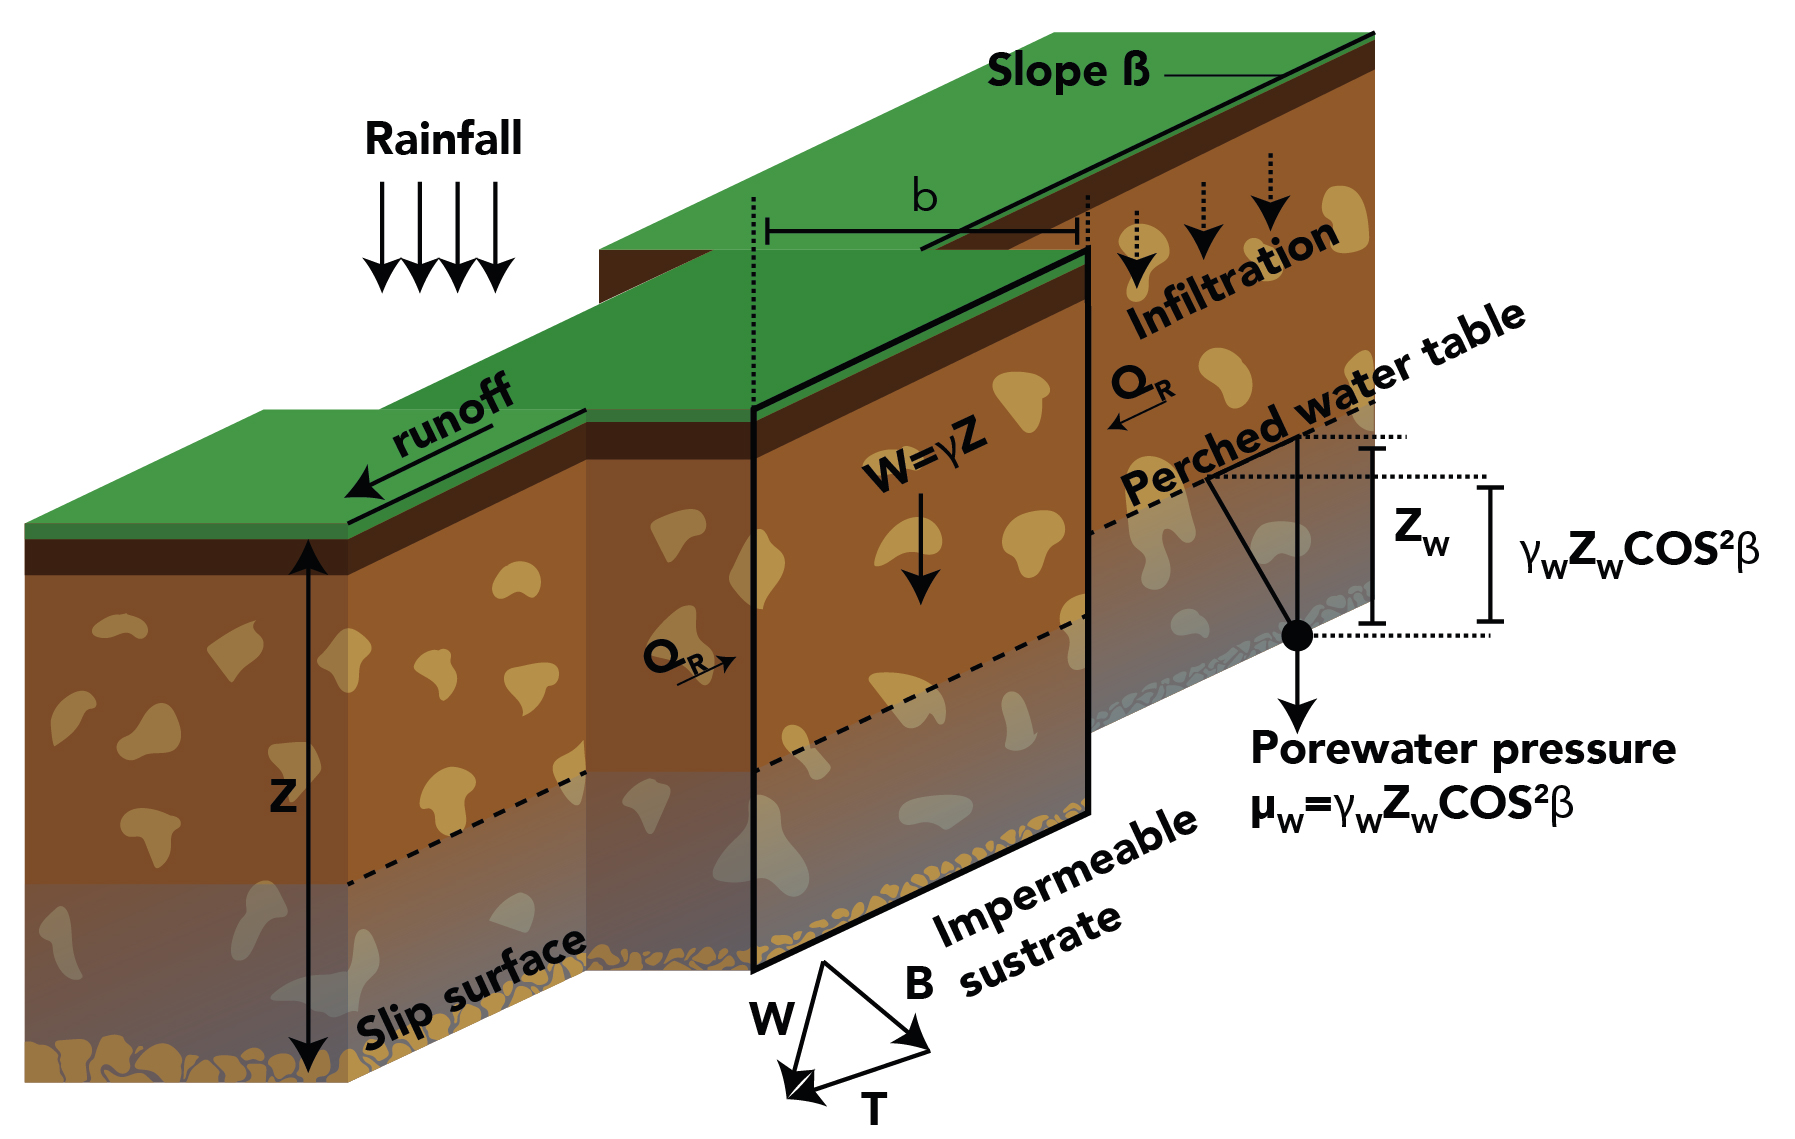
\includegraphics[width=8.3cm]{Figures/slides-escheme.jpg}
 \caption{\DIFdelbeginFL \DIFdelFL{The }\DIFdelendFL \DIFaddbeginFL \DIFaddFL{Schematic diagram of the }\DIFaddendFL geotechnical conceptual model. \DIFdelbeginFL \DIFdelFL{Figure }\DIFdelendFL \DIFaddbeginFL \DIFaddFL{The figure }\DIFaddendFL and description are adapted from \citet{Aristizabal2016}. \DIFaddbeginFL \DIFaddFL{$Q_L$ and $Q_R$ are the resultant forces on the sides of the slice. }\DIFaddendFL }
    \label{fig:ModeloEstabilidad}
\end{figure}

\DIFdelbegin \begin{displaymath}
 \DIFdel{Z_{i,min} = \frac{C^{'}}{\gamma_w cos^2 \beta tan \phi + \gamma cos^2 \beta (tan\beta - tan \phi)}
    %DIFDELCMD < \label{eq:zmin}%%%
}\end{displaymath}
%DIFAUXCMD
\begin{displaymath}
 \DIFdel{Z_{i,max} = \frac{C^{'}}{\gamma cos^2 \beta (tan\beta - tan \phi)}
 %DIFDELCMD < \label{eq:zmax}%%%
}\end{displaymath}
%DIFAUXCMD
\begin{displaymath}
 \DIFdel{\beta_{i,0} = tan ^{-1} \left[ tan \phi \left( 1- \frac{\gamma_w}{\gamma}\right) \right]
 %DIFDELCMD < \label{eq:bo}%%%
}\end{displaymath}
%DIFAUXCMD
%DIFDELCMD < 

%DIFDELCMD < %%%
\DIFdel{The model assess conditionally stable cells in function of their perched water table for each cell ($Z_{i,w}$, equation \ref{eq:z}) and the critical satured depth ($Z_{i,c}$, equation (\ref{eq:Zcrit})).  Slope failure occurs when $Z_{i,w}$ is greater than $Z_{i,c}$. At equation (\ref{eq:z}) $S_{3,i}$ represents gravitational storage, $Ws$ and $W_{fc}$ the soil saturation and field capacity respectively. And in equation (\ref{eq:Zcrit}) $C^{'}$ represents the soil cohesion and $\beta$ the cell slope.
}%DIFDELCMD < 

%DIFDELCMD < %%%
\begin{displaymath}
 \DIFdel{Z_{i,w}(t) = \frac{S_{3,t}}{W_c - W_{fc}}
 %DIFDELCMD < \label{eq:z}%%%
}\end{displaymath}
%DIFAUXCMD
\begin{displaymath}
 \DIFdel{Z_{i,c} = \frac{\gamma}{\gamma_w} Z \left( 1-\frac{tan \beta}{tan\phi} \right)
     + \frac{C^{'}}{\gamma_w cos^2 \beta tan\phi}
 %DIFDELCMD < \label{eq:Zcrit}%%%
}\end{displaymath}
%DIFAUXCMD
\DIFdelend \DIFaddbegin \begin{table}[]
        \centering
        \begin{tabularx}{\textwidth}{p{3cm} p{2.2cm} p{1.5cm} p{2cm} p{3.5cm}}
\hline
\DIFaddFL{Parameter Name }& \DIFaddFL{Symbol }& \DIFaddFL{Scalar Parameter }& \DIFaddFL{Mean Value }& \DIFaddFL{Spatial distribution }\\
\hline
\DIFaddFL{Soil depth }& \DIFaddFL{$Z_i$ }[\DIFaddFL{mm}] & \DIFaddFL{0.3 }& \DIFaddFL{300 }& \DIFaddFL{As a function of the slope }\\
\DIFaddFL{Topography slope }& \DIFaddFL{$\beta_{i,0}$ }[\DIFaddFL{adim}] & \DIFaddFL{1 }& \DIFaddFL{0.01 - 5.3 }&  \DIFaddFL{From the DEM }\\
\DIFaddFL{Soil bulk density }& \DIFaddFL{$\gamma_i$ }[\DIFaddFL{$KNm^{-3}$}] & \DIFaddFL{1  }& \DIFaddFL{18  }& \DIFaddFL{Assumed constant}\\
\DIFaddFL{Water density }& \DIFaddFL{$\gamma_w$ }[\DIFaddFL{$KNm^{-3}$}] & \DIFaddFL{1 }& \DIFaddFL{9.8 }& \DIFaddFL{Constant}\\
\DIFaddFL{Soil stability angle }& \DIFaddFL{$\phi_i$ }[\DIFaddFL{$^0$}] & \DIFaddFL{1 }& \DIFaddFL{30$^0$ }& \DIFaddFL{Assumed constant}\\
\DIFaddFL{Soil cohesion }& \DIFaddFL{$C^{'}_i$ }[\DIFaddFL{KN}] & \DIFaddFL{1 }& \DIFaddFL{4 }& \DIFaddFL{Assumed constant}\\
\hline
\end{tabularx}
\caption{\DIFaddFL{Shallow landslides model parameters.}}
\label{tab:landslide}
\end{table}
\DIFaddend 

\subsection{\DIFdelbegin \DIFdel{Flash flood submodel (}\DIFdelend HydroFlash\DIFdelbegin \DIFdel{)}\DIFdelend }

In this \DIFdelbegin \DIFdel{work, we introduce a low-cost 1D hydraulic }\DIFdelend \DIFaddbegin \DIFadd{section, we describe the HydroFlash flash }\DIFaddend model for flash \DIFdelbegin \DIFdel{flood simulation referred to as HydroFlash}\DIFdelend \DIFaddbegin \DIFadd{floods}\DIFaddend . The model extracts the cross-profile from the DEM for each cell considered part of the network,  \DIFdelbegin \DIFdel{estimating }\DIFdelend \DIFaddbegin \DIFadd{and it estimates }\DIFaddend flood spots at each network cell during execution time.\\

The model requires hydraulic parameters for all network cells to determine flash-flooding spots. \DIFdelbegin \DIFdel{Channel }\DIFdelend \DIFaddbegin \DIFadd{The channel }\DIFaddend width is estimated using the \cite{Leopold1953} approach $ W_i = 3.26 \overline{Q_i}^{0.469}$. \DIFdelbegin \DIFdel{Channel }\DIFdelend \DIFaddbegin \DIFadd{The channel }\DIFaddend slope ($S_{i,0}$) is obtained as the mean value of the slopes that correspond to the cells of a hydrological reach. The characteristic  \DIFdelbegin \DIFdel{particle }\DIFdelend diameter $D_{i,50}$ is assumed equal to 0.138 $m$ and constant \citep{Golden2006}. The cross-section (\DIFdelbegin \DIFdel{$C_s$}\DIFdelend \DIFaddbegin \DIFadd{$F_{sec,i}$}\DIFaddend ) is obtained from the DEM \DIFdelbegin \DIFdel{, }\DIFdelend for every network cell, perpendicular to the flow direction of the cell\DIFdelbegin \DIFdel{(}\DIFdelend \DIFaddbegin \DIFadd{, }\DIFaddend $D8_{i}$\DIFaddbegin \DIFadd{,  (see step 1 in Figure \ref{fig:hydroflash}}\DIFaddend ).\\

For each time step $t$ and for each stream cell, equation \ref{eq:altura} determines the height of the water table $Y_{i}(t)$ using the simulated streamflow $Q_{i,sim}(t)$ and flow velocity $v_{i,sim}(t)$ \DIFaddbegin \DIFadd{(step 2 in Figure \ref{fig:hydroflash})}\DIFaddend . The model calculates the friction velocity ($v_{fr,i}(t)$) using $Y_i(t)$ as in equation (\ref{eq:velocidad}) derived from Keulegan and Rouse equations \citep{takahashi1991, Savage1984}. Equations \ref{eq:con} and \ref{eq:rdf} allow the estimation of the concentration ($c_{i}(t)$) and constitutive coefficients ($r_{i}(t)$), respectively. \DIFaddbegin \DIFadd{The constitutive coefficient summarizes the dynamics associated with flows containing colliding particles, such as a flash flood \mbox{%DIFAUXCMD
\citep{takahashi1991}}\hspace{0pt}%DIFAUXCMD
. In general, the characteristics of an apparent fluid are determined by the relationship between the operating shear stress and the rate of strain, known as the constitutive law. }\DIFaddend In equation \ref{eq:con}\DIFaddbegin \DIFadd{, }\DIFaddend $C_{max}$ represents the maximum sediment concentration; according to \citet{Obrien1988} $C_{max}$ is near 0.75 during flash floods. The \DIFdelbegin \DIFdel{stream flow }\DIFdelend \DIFaddbegin \DIFadd{streamflow }\DIFaddend plus estimated sediments and rubble \DIFdelbegin \DIFdel{is }\DIFdelend \DIFaddbegin \DIFadd{are }\DIFaddend estimated according to equation \ref{eq:qescombros}.

\begin{equation}
 Y_i(t) = \frac{Q_{i,sim}(t)}{v_{i,sim}(t) w_{i}}
 \label{eq:altura}
\end{equation}
\begin{equation}
 v_{fr,i}(t) = \frac{v_{i,sim}(t)}{5.75 log \left( \frac{Y_{i}(t)}{D_{i,50}} \right) + 6.25}
 \label{eq:velocidad}
\end{equation}
\begin{equation}
 c_{i}(t) = C_{max} (0.06 Y_{i}(t))^{\frac{0.2}{v_{fr,i}(t)}}
 \label{eq:con}
\end{equation}
\begin{equation}
r_{i}(t) = \frac{1}{D_{i,50}} \left [ \frac{g}{0.0128} \left( c_i+(1-c_i) \frac{\gamma_w}{\gamma_{sed}} \right ) \right ]^{1/2} \cdot \left[ \left( \frac{C_{max}}{c_i} \right )^{1/3} -1\right ]
 \label{eq:rdf}
\end{equation}
\begin{equation}
 Q_{i,sed}(t) = \frac{Q_{i,sim}(t)}{1-c_i(t)}
 \label{eq:qescombros}
\end{equation}

Assuming \DIFaddbegin \DIFadd{an }\DIFaddend infinite sediment and rubble supply, $Q_{i,sed}(t)$ \DIFdelbegin \DIFdel{is the maximum stream flow for the section.  To determine the flooded area, a }\DIFdelend \DIFaddbegin \DIFadd{corresponds to the maximum streamflow for each section.  The }\DIFaddend flood depth $F_{d,i}(t)$ \DIFdelbegin \DIFdel{must be found in order to obtain an stream flow ($\hat{Q}_{{i,sed}(t)}$) (equation \ref{eq:constitutiva}) that equals $Q_{i,sed}(t)$.  The search of $F_{d,i}$ is done iteratively by making small increments to it.  Both flooded area ($A_{i,sed}(t)$) and flooded section ($F_{f,i}$) are obtained in the process.  At each iteration, $F_{d,i}$ is an estimated depth (equation }\DIFdelend \DIFaddbegin \DIFadd{is computed following equation (}\DIFaddend \ref{eq:elevacion}), \DIFdelbegin \DIFdel{measured from the bottom of the section ($b_i$) to a guess elevation of the section ($\Delta y \cdot j$) .  The depth of $F_{d,i}$ increases with each iteration as $j$ takes values between 1 and the total number of iterations with a step of 1.  At the end of each iteration, $A_{i,sed}(t)$ is estimated with equation \ref{eq:differencia}, in which $F_{sec,i}$ corresponds to the section $i$ extracted from the DEM. Based on the value obtained for $A_{i,sed}(t)$}\DIFdelend \DIFaddbegin \DIFadd{iteratively, such that the difference between the estimated stream flow ($\hat{Q}{{i,sed}(t)}$) (equation \ref{eq:constitutiva}) and the simulated streamflow $Q{i,sed}(t)$ is less than a predetermined admissible error $\sigma$ (step 2 in Figure \ref{fig:hydroflash}). In the process}\DIFaddend , the model \DIFdelbegin \DIFdel{estimates $\hat{Q}_{i,sed}$ (equation \ref{eq:constitutiva}).  The process stops when $\hat{Q}_{i,sed}$ is similar to $Q_{i,sed}$, at this point}\DIFdelend \DIFaddbegin \DIFadd{obtains the flooded area $A_{i,sed}$ (equation (\ref{eq:differencia}))}\DIFaddend , the flooded \DIFaddbegin \DIFadd{cells for each¡ }\DIFaddend section $F_{f,i}$ \DIFdelbegin \DIFdel{corresponds to the values of $F_{sec,i}$ that are below $F_{d,i}$}\DIFdelend \DIFaddbegin \DIFadd{and the flood depth (step 3 in Figure \ref{fig:hydroflash})}\DIFaddend .  

 \begin{equation}
     F\DIFdelbegin \DIFdel{_{d,i} }\DIFdelend \DIFaddbegin \DIFadd{_{d,i,j} }\DIFaddend = b_i + \Delta y \cdot j
     \label{eq:elevacion}
 \end{equation}

 \begin{equation}
  \hat{A}_{i,sed} = \Delta x \sum_{j=1}^{N} F_{d,i} - F_{sec,i} 
  \label{eq:differencia}
 \end{equation}

 \begin{equation}
   \hat{Q}_{i,sed}(t) = \left( \frac{2}{5} \right) r_i(t)(j \Delta y)^{\frac{3}{2}} S_{0,i} \hat{A}_{i,sed}(t) \cdot 0.5
 \label{eq:constitutiva} 
 \end{equation}

\DIFdelbegin \DIFdel{Resulting }\DIFdelend \DIFaddbegin \DIFadd{The resulting }\DIFaddend flood maps might \DIFdelbegin \DIFdel{evidence }\DIFdelend \DIFaddbegin \DIFadd{include }\DIFaddend the presence of small isolated flood spots and discontinuities \DIFdelbegin \DIFdel{at flood spots where }\DIFdelend \DIFaddbegin \DIFadd{where the }\DIFaddend flow direction changes from orthogonal to diagonal or \DIFdelbegin \DIFdel{vice-versa}\DIFdelend \DIFaddbegin \DIFadd{vice versa}\DIFaddend . We included two post-processing steps to correct these issues by (i) using an image processing erosion algorithm \citep{Serra1983} to remove the small isolated flood spots \DIFdelbegin \DIFdel{. The }\DIFdelend \DIFaddbegin \DIFadd{(step 4 in Figure \ref{fig:hydroflash}); the image }\DIFaddend erosion is performed once with a \DIFdelbegin \DIFdel{3x3 kernel, and (ii) to }\DIFdelend \DIFaddbegin \DIFadd{3 by 3 kernel. To }\DIFaddend solve the flow direction discontinuities, \DIFaddbegin \DIFadd{(ii) }\DIFaddend each flooded cell seeks to \DIFdelbegin \DIFdel{flood }\DIFdelend \DIFaddbegin \DIFadd{inundate }\DIFaddend its eight neighboring cells. A neighbor cell is also flooded if the altitude of the original flooded cell\DIFaddbegin \DIFadd{, }\DIFaddend plus the flood depth\DIFaddbegin \DIFadd{, }\DIFaddend is higher than its elevation \DIFdelbegin \DIFdel{.
}\DIFdelend \DIFaddbegin \DIFadd{(step 5 in Figure \ref{fig:hydroflash}). An example of the final result for a time step $t$ is shown in the step 6 in Figure \ref{fig:hydroflash}.
}

\begin{figure}[t]
\centering
 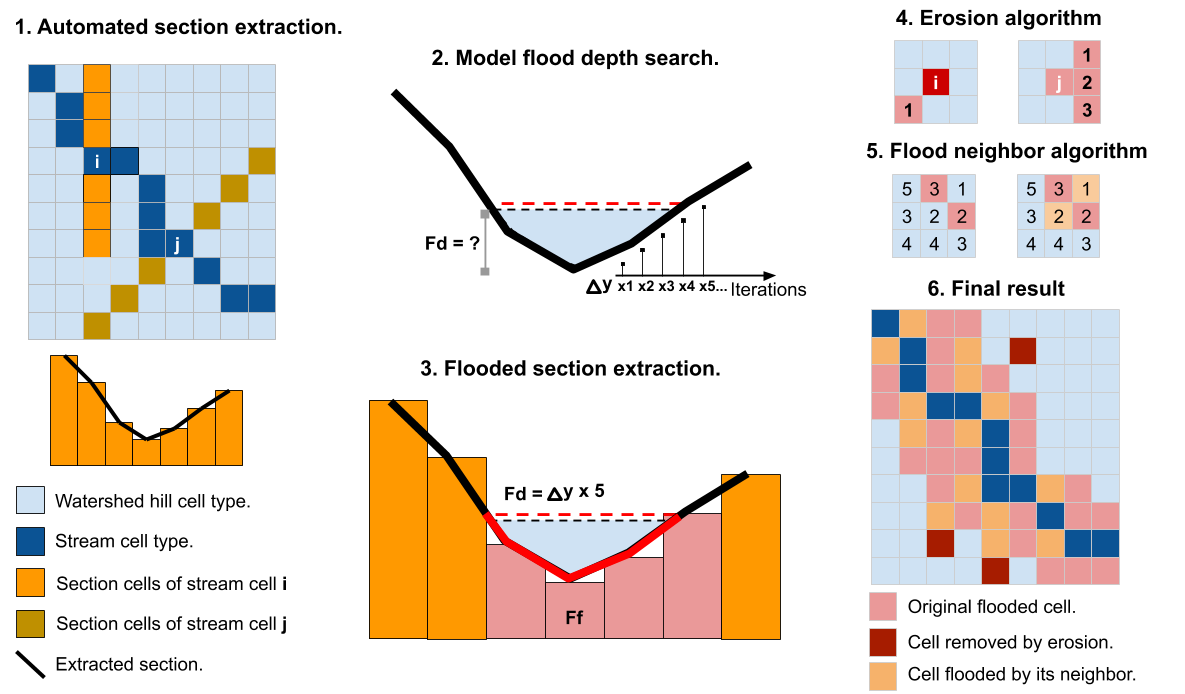
\includegraphics[width=12cm]{Figures/HydroFlash_scheme.png}
 \caption{\DIFaddFL{HydroFlash submodel scheme. 1. The model }\textbf{\DIFaddFL{wmf}} \DIFaddFL{extracts the cross-profile from the network. 2. With equation (\ref{eq:constitutiva}), the model obtains a first approximation to the flash flood streamflow; then, the flood depth and area are obtained with equations (\ref{eq:elevacion}) to (\ref{eq:constitutiva}). 3. The model obtains the flooded portion of the cross section. 4. Erosion post-process. 5. Filling post-process. 6. The final result is acquired for a time step $t$.}}
    \label{fig:hydroflash}
\end{figure}
\DIFaddend 

%%-----------------------------------------------------------
%%-----------------------------------------------------------
%Results
%%-----------------------------------------------------------
%%-----------------------------------------------------------
\section{Results}
\label{sec:results}

The primary results of the present study include the reconstruction of the 2015 Salgar flash flood, the assessment of the importance of soil moisture in the hydrologic response of the basin, and the evaluation of the relative role of stratiform and convective precipitation cores in the generation of the observed extreme event. This section is based on the results from the analysis of the hydrological simulation, as well as \DIFaddbegin \DIFadd{occurrences of }\DIFaddend shallow landslides and flash floods \DIFdelbegin \DIFdel{occurrence }\DIFdelend and simulation. \\

\subsection{Hydrologic model validation and sensitivity analysis}

Figure \ref{fig:SimStreamflow}a presents the results of the hydrological simulation at the outlet of the basin.  The \DIFdelbegin \DIFdel{model simulation is set to reach a base flow of 3 m$^3 \text{s}^{-1}$, a value that corresponds to the discharge measurements during field campaigns days and weeks after the flash flood event and during dry spells.   The }\DIFdelend simulation shows that Event 1 generates a hydrograph with a peak flow of $Q_{max}$ = 160 m$^3 \text{s}^{-1}$. It is important to note that during precipitation \DIFaddbegin \DIFadd{in }\DIFaddend Event 1\DIFaddbegin \DIFadd{, }\DIFaddend there were no damage \DIFdelbegin \DIFdel{nor }\DIFdelend \DIFaddbegin \DIFadd{or }\DIFaddend flooding reports by local authorities. Even though this precipitation event did not generate flooding, it set wet conditions in the entire basin before the occurrence of Event 2 (see the purple line in Figure \ref{fig:SimStreamflow}b). Additionally, it is clear from the simulation that during the flash flood event\DIFaddbegin \DIFadd{, }\DIFaddend the two successive convective cores over the same region (training convection) generated a peak flow of $Q_{max}$ =220 m$^3 \text{s}^{-1}$, \DIFaddbegin \DIFadd{a }\DIFaddend value that is in the upper range of the estimated streamflow based on post-event field evidence (185-222 m$^3 \text{s}^{-1}$). Figure \ref{fig:SimStreamflow}a also presents the simulated runoff and subsurface flow separation as well as the \DIFdelbegin \DIFdel{convective-stratiform generated }\DIFdelend \DIFaddbegin \DIFadd{convective-stratiform-generated }\DIFaddend discharge discrimination. The modeling evidence during Event 2 suggests the convective rainfall fraction dominates the hydrograph formation. In both events, convective (stratiform) precipitation appears to be closely related to the simulated runoff (subsurface flow). On the other hand, the simulated subsurface flow is more important in magnitude than \DIFaddbegin \DIFadd{that }\DIFaddend runoff in describing Event 1, while runoff is more relevant for Event 2. Figure \ref{fig:SimStreamflow}b presents \DIFaddbegin \DIFadd{the }\DIFaddend capillary storage (purple), as well as \DIFaddbegin \DIFadd{the }\DIFaddend runoff (continuous blue) and \DIFaddbegin \DIFadd{the }\DIFaddend gravitational (dashed blue) storage temporal variability \DIFaddbegin \DIFadd{as represented by the proposed model}\DIFaddend . As expected, runoff storage is only \DIFdelbegin \DIFdel{non-zero }\DIFdelend \DIFaddbegin \DIFadd{nonzero }\DIFaddend during the storm duration, while gravitational storage increases considerably during rain events, followed by a slow recession. There is an \DIFdelbegin \DIFdel{increment of }\DIFdelend \DIFaddbegin \DIFadd{increase in }\DIFaddend basin-wide capillary storage during Event 1, remaining considerably high \DIFaddbegin \DIFadd{during }\DIFaddend the time leading to the occurrence of Event 2. According to the model simulations, the peak flow occurred \DIFdelbegin \DIFdel{around }\DIFdelend \DIFaddbegin \DIFadd{at approximately }\DIFaddend 2:20 a.m. \DIFaddbegin \DIFadd{LT }\DIFaddend on May 18th, which is very accurate compared to the reports from local authorities \DIFaddbegin \DIFadd{(2:40 a.m. LT) }\DIFaddend considering all the data limitations.\\


\begin{figure}[t]
\centering
 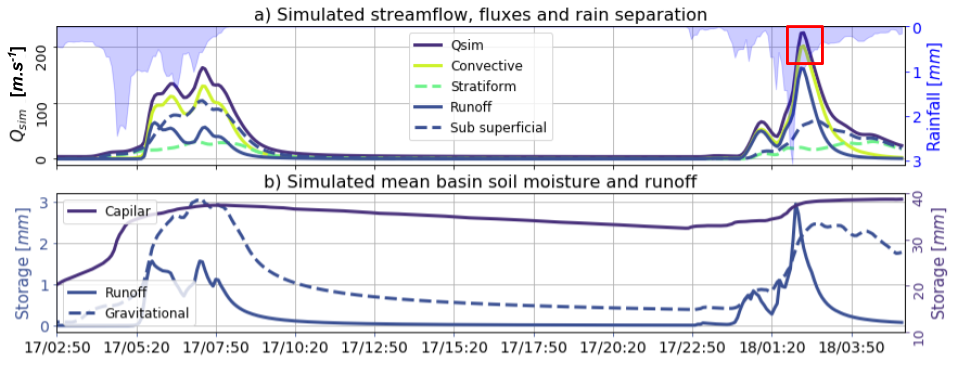
\includegraphics[width=12cm]{Figures/Caudal_Sim_v2.png}
 \caption{Summary of the \DIFdelbeginFL \DIFdelFL{Results }\DIFdelendFL \DIFaddbeginFL \DIFaddFL{results }\DIFaddendFL from the hydrological simulation. a) Simulated streamflow, runoff and \DIFdelbeginFL \DIFdelFL{sub-surface }\DIFdelendFL \DIFaddbeginFL \DIFaddFL{subsurface }\DIFaddendFL flow separation and \DIFdelbeginFL \DIFdelFL{convective-stratiform generated }\DIFdelendFL \DIFaddbeginFL \DIFaddFL{convective-stratiform-generated }\DIFaddendFL discharge discrimination. The red square represents the flash flood peakflow interval \DIFaddbeginFL \DIFaddFL{that is }\DIFaddendFL estimated based on field \DIFdelbeginFL \DIFdelFL{campaing }\DIFdelendFL \DIFaddbeginFL \DIFaddFL{campaign }\DIFaddendFL evidence. b) \DIFdelbeginFL \DIFdelFL{Mean }\DIFdelendFL \DIFaddbeginFL \DIFaddFL{The mean }\DIFaddendFL runoff, gravitational, and capillary storages during the simulation period.}
    \label{fig:SimStreamflow}
\end{figure}

Figure \ref{fig:SimStreamflowSA} shows the results of a sensitivity analysis of the hydrological simulation during the second rainfall event, varying the infiltration rate, and the surface and subsurface speed parameters. The aim of the sensitivity analysis is to evaluate the robustness of the overall results, considering the fact that the quality and quantity of some of the watershed information is limited. \DIFaddbegin \DIFadd{In the sensitivity analysis, we vary the infiltration parameter between 0.02 and 20, the surface speed parameter between 0.01 and 20, and the subsurface speed parameter between 0.1 and 10. }\DIFaddend The overall simulation sensitivity results show \DIFaddbegin \DIFadd{that }\DIFaddend the main findings described in the previous paragraphs are, in fact, robust to almost all changes in the mentioned parameters, with \DIFdelbegin \DIFdel{surface runoff }\DIFdelend \DIFaddbegin \DIFadd{the surface runoff that is }\DIFaddend associated with convective rainfall controlling the magnitude of the peak discharge during the Event 2. Changes in the infiltration rate (Figure \ref{fig:SimStreamflowSA}a) result in peak flow changes with a magnitude less than 7\%,  and changes in the subsurface velocity parameter (Figure \ref{fig:SimStreamflowSA}c) lead to peak flow changes with a magnitude less than 20\% \DIFaddbegin \DIFadd{in }\DIFaddend the original simulation. The model\DIFaddbegin \DIFadd{'s }\DIFaddend highest sensitivity, and hence the largest uncertainty source, appears to be related to the surface speed parameter (Figure \ref{fig:SimStreamflowSA}b), particularly \DIFdelbegin \DIFdel{in the low-end values. Although some of the surface speed valuesused in the analysis are unrealistically low, it is noteworthy to report that these values lead to the attenuation of the hydrograph and the reduction of the peak flow. }\DIFdelend \DIFaddbegin \DIFadd{during the peak flow and early recession. }\DIFaddend \\

\begin{figure}[t]
\centering
 \DIFdelbeginFL %DIFDELCMD < 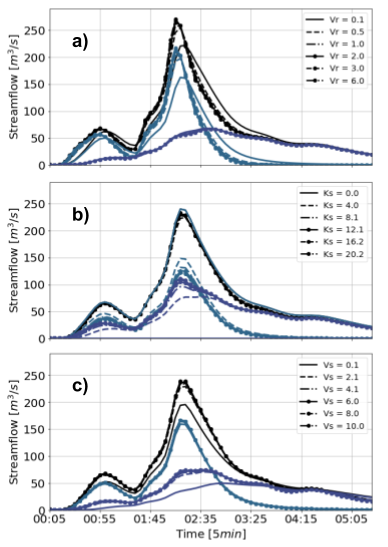
\includegraphics[width=14cm]{Figures/Parameter_variation_analysis.png}
%DIFDELCMD <  \caption{%%%
\DIFdelFL{Hydrological simulation sensitivity analysis. Similarly as in Figure \ref{fig:SimStreamflow}}\DIFdelendFL \DIFaddbeginFL 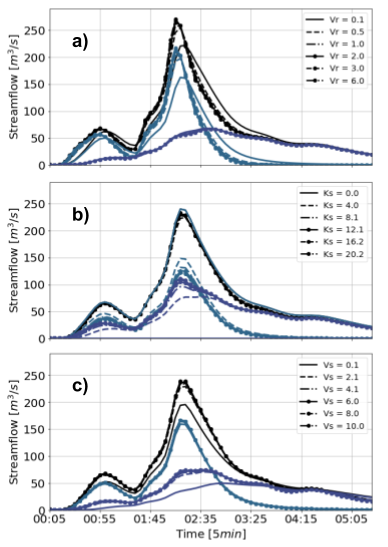
\includegraphics[width=7cm]{Figures/Parameter_variation_analysis.png}
 \caption{\DIFaddFL{Hydrological simulation sensitivity analysis. Similarly as in Figure \ref{fig:SimStreamflow}, all panels show the simulated streamflow, and the runoff and subsurface flow separation. Total streamflow is purple, runoff is green and subsurface dashed purple. The left panel shows sensitivity to changes in the infiltration rate  parameter, the middle panel to changes in surface speed, and the right panel to changes in subsurface speed.}}
    \label{fig:SimStreamflowSA}
\end{figure}

\DIFadd{After the flash flood event, SIATA installed a stream gauge level station near the outlet of the basin (see Figure \ref{fig:Ubicacion}).  We use these records to validate the model results without further calibration. Since the observed series correspond to level values, the streamflow estimation is performed following two different approaches. The first approach, the empirical one, consists of subtracting the 10th percentile of the observed stage time series from the observational record, and the 10th percentile of the simulated streamflow, from the same series.  On the other hand, the second method uses the Manning formula.  For this, we consider the geometry of the section in Figure \ref{fig:Seccion}, and the slope from the DEM.  Additionally, due to the potential uncertainties, we consider three different Manning values (0.015}\DIFaddend , \DIFdelbegin \DIFdel{all panels show the simulated streamflow}\DIFdelend \DIFaddbegin \DIFadd{0.02}\DIFaddend , \DIFaddbegin \DIFadd{0.03). Figure \ref{fig:validacion} shows the estimated streamflow using the two methods for four different hydrographs during July, August (2 events) and December 2015. The simulated magnitudes appear relatively close to the observations, and the peak discharge time is captured skillfylly in three of the four cases presented. The discharge values using the "high" Manning number estimation (0.015) are similar to the empirical method. The performance of the model is acceptable (Figure \ref{fig:validacion}), considering the lack of calibration, the size of the basin, and the magnitude of the recorded events.  The results shown include cases where the peak flow was over-estimated (panels c and d), and  under-estimated (panel b).
}

\begin{figure}[t]
\centering
 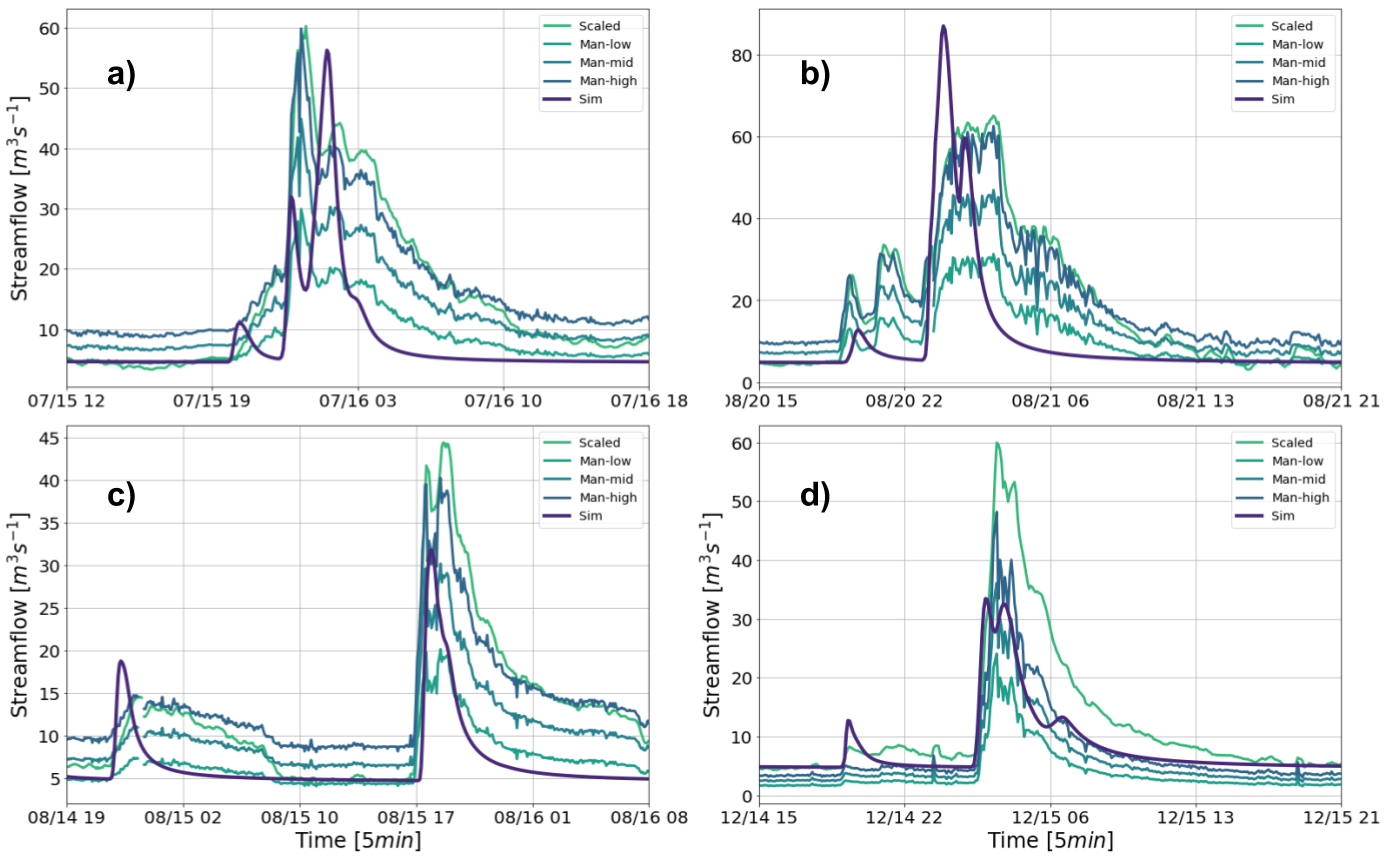
\includegraphics[width=10cm]{Figures/Eventos_Validacion.png}
 \caption{\DIFaddFL{Comparison between hydrological model simulations }\DIFaddendFL and \DIFdelbeginFL \DIFdelFL{the runoff and sub-surface flow separation}\DIFdelendFL \DIFaddbeginFL \DIFaddFL{streamflow estimations}\DIFaddendFL . The \DIFdelbeginFL \DIFdelFL{left panel shows sensitivity to changes in the infiltration rate  parameter, }\DIFdelendFL \DIFaddbeginFL \DIFaddFL{events were observed by a level station installed by SIATA days after Event 2 on a bridge at }\DIFaddendFL the \DIFdelbeginFL \DIFdelFL{middle panel to changes in surface speed, and }\DIFdelendFL \DIFaddbeginFL \DIFaddFL{outlet of }\DIFaddendFL the \DIFdelbeginFL \DIFdelFL{right panel to changes in subsurface speed.}\DIFdelendFL \DIFaddbeginFL \DIFaddFL{basin (see Figure \ref{fig:Ubicacion})}\DIFaddendFL }
    \DIFdelbeginFL %DIFDELCMD < \label{fig:SimStreamflowSA}
%DIFDELCMD < %%%
\DIFdelendFL \DIFaddbeginFL \label{fig:validacion}
\DIFaddendFL \end{figure}


Figure \ref{fig:dischargeEvent2} shows the temporal evolution of discharge during Event 2 in different locations along the watershed's main channel. The upper location corresponds to 15\% of the area of the basin, and the other downstream locations \DIFaddbegin \DIFadd{correspond }\DIFaddend to 52\%, 76\%, and 100\% of the watershed\DIFdelbegin \DIFdel{, respectively}\DIFdelend \DIFaddbegin \DIFadd{. The difference in the time of the peak discharge between the upper location and the outlet of the basin is approximately $35min$, which is plausible with travel speeds between 5 and 7 ms$^{-1}$ and an effective distance of 14$km$}\DIFaddend .  In terms of volume, \DIFdelbegin \DIFdel{73 Mm}\DIFdelend \DIFaddbegin \DIFadd{approximately 737,000 m}\DIFaddend $^3$ of the total \DIFdelbegin \DIFdel{144 Mm}\DIFdelend \DIFaddbegin \DIFadd{1,438,000 m}\DIFaddend $^3$ simulated at the outlet of the basin are generated on the 15\% upstream part of the watershed,  corresponding to about half of the total mass. In terms of peak flow, due to the slope and velocity changes, the simulated discharge at the 15\% upstream part of the watershed corresponds to \DIFdelbegin \DIFdel{61}\DIFdelend \DIFaddbegin \DIFadd{50}\DIFaddend \% of the peak discharge at the outlet of the basin.\\

\begin{figure}[t]
\centering
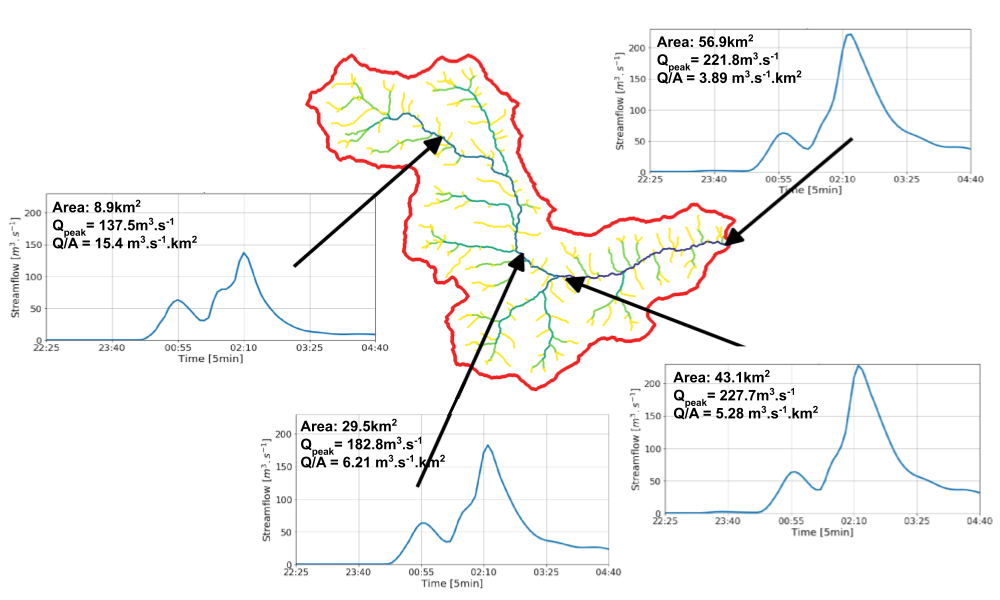
\includegraphics[width =12cm]{Figures/Evolucion_evento.png}
\caption{Temporal evolution of discharge during Event 2 in different locations along the watershed's main channel. The upper location corresponds to 15\% of the area of the basin, and the other downstream locations \DIFaddbeginFL \DIFaddFL{correspond }\DIFaddendFL to 52\%, 76\%, and 100\% of the watershed, respectively.}
\label{fig:dischargeEvent2}
\end{figure}

\subsection{Flash flood processes}

\DIFdelbegin \DIFdel{In this study, we propose a graphical method to assess the soil-rainfall-discharge coupling holistically. The first step is to classify all the cells within the watershed in a predetermined number of groups according to their localization and the distance to the outlet. The aim is to establish a coherent and robust spatial discretization, thus allowing to summarize the concurrent spatio-temporal variability of the different processes in 2D diagrams.}%DIFDELCMD < \\
%DIFDELCMD < 

%DIFDELCMD < %%%
\DIFdelend % \begin{figure}[t]
% \centering
% 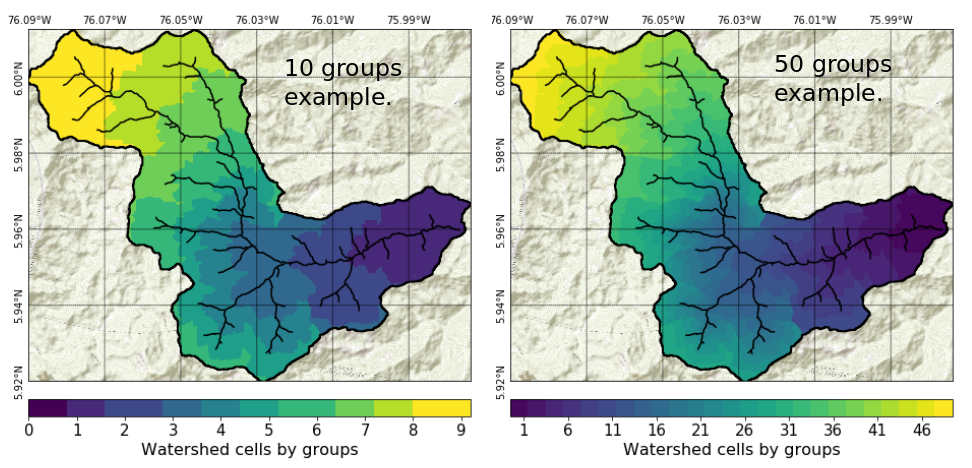
\includegraphics[width=8.3cm]{Figures/Mapas_Grupos.png}
% \caption{Example of watershed grouping as a function of distance to the outlet for La Liboriana basin. The left panel corresponds to clustering using ten different groups, and the right panel shows the 50-groups categorization used in the present study.}
% \label{fig:ExplainationGroups}
% \end{figure}

Figure \ref{fig:HumedadSpatioTemporal} presents the proposed 2D diagrams obtained for the simulation of the La Liboriana basin flash flood using a spatial discretization with 50 groups. Figure \ref{fig:HumedadSpatioTemporal}a includes the evolution of the average rainfall over the basin (black line), and the \DIFdelbegin \DIFdel{spatio-temporal }\DIFdelend \DIFaddbegin \DIFadd{spatiotemporal }\DIFaddend evolution of capillary storage (filled isolines) and return flow (colored isolines from white to red) by groups. For the analysis, it is relevant to highlight that higher numbered groups are located away from the outlet of the basin and correspond in this case to considerably steeper slopes. Figure \ref{fig:HumedadSpatioTemporal}b presents the evolution of streamflow at the outlet of the basin (black line)\DIFaddbegin \DIFadd{, }\DIFaddend as well as the gravitational storage (filled isolines) and runoff (colored isolines) \DIFdelbegin \DIFdel{spatio-temporal }\DIFdelend \DIFaddbegin \DIFadd{spatiotemporal }\DIFaddend evolution. Figure \ref{fig:HumedadSpatioTemporal} shows variations in the capillary and gravitational storages associated with Event 1 in the higher numbered groups. The capillary storage remains high in almost all the basin until the start of Event 2. According to the conceptualization of the model, the gravitational storage and surface runoff start to interact when the capillary storage is full. In this case, this situation is set up by Event 1. \DIFdelbegin \DIFdel{Model }\DIFdelend \DIFaddbegin \DIFadd{The model }\DIFaddend runs for Event 2 using dry initial states, \DIFdelbegin \DIFdel{show }\DIFdelend \DIFaddbegin \DIFadd{showing }\DIFaddend no flooding in the results.\\

\begin{figure}[t!]
\centering
 \DIFdelbeginFL %DIFDELCMD < 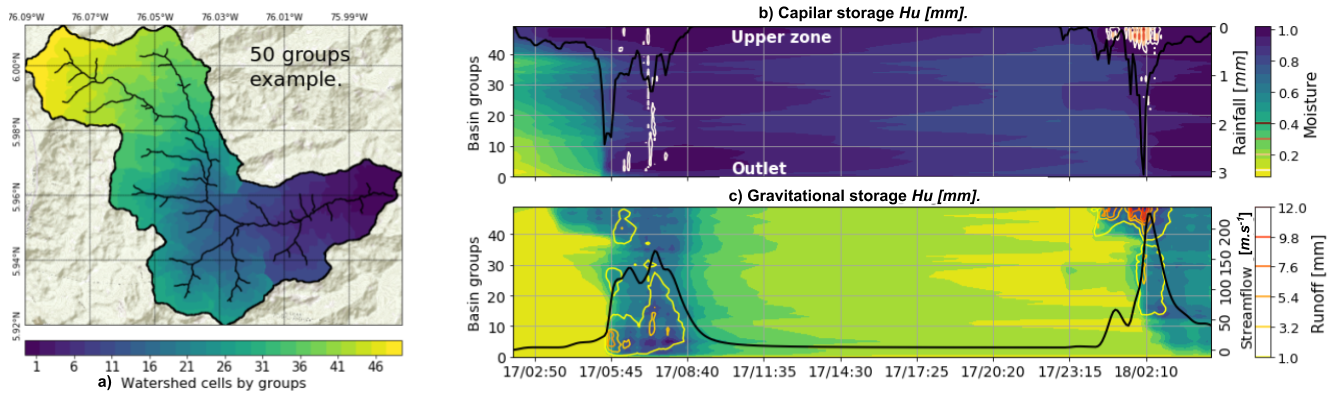
\includegraphics[width=12cm]{Figures/Figure_9_10.png}
%DIFDELCMD <  %%%
\DIFdelendFL \DIFaddbeginFL 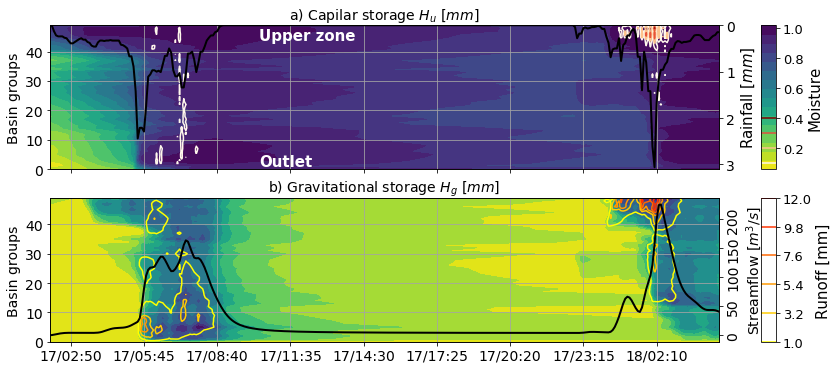
\includegraphics[width=14cm]{Figures/Evolucion_humedad.png}
 \DIFaddendFL \caption{\DIFdelbeginFL \DIFdelFL{Watershed groups and spatiotemporal analysis of Events 1 and 2.  a) Example of watershed grouping as a function of of their localization and distance to the outlet for La Liboriana basin using a 50-groups categorization. Each group corresponds to }\DIFdelendFL  a\DIFdelbeginFL \DIFdelFL{row in the contour plots b) and c). b}\DIFdelendFL ) Simulated capillary moisture (filled green-to-blue contours) and returned flow occurrence (white to red isolines).  The black line represents the average rainfall over the basin. \DIFdelbeginFL \DIFdelFL{c}\DIFdelendFL \DIFaddbeginFL \DIFaddFL{b}\DIFaddendFL ) Simulated gravitational moisture (filled green-to-blue contours) and runoff (yellow-to-red isolines).  The black line represents streamflow at the outlet of the basin.  The green-to-blue color bar serves as a reference for capillary moisture and gravitational water content.}
    \label{fig:HumedadSpatioTemporal}
\end{figure}

\DIFdelbegin \DIFdel{It is well known that the }\DIFdelend \DIFaddbegin \DIFadd{The }\DIFaddend temporal variability of rainfall intensity plays an important role in the hydrograph structure. During Event 1\DIFaddbegin \DIFadd{, }\DIFaddend rainfall accumulated over the basin at a relatively stable rate (Figure \ref{fig:lluviaElapsedCaudal}a). On the other hand, Event 2 presents a significant increase in rainfall rate in the second half of the life cycle (Figure \ref{fig:lluviaElapsedCaudal}b). This change in precipitation intensity is associated with a considerable intensification of the training convective cores due to orographic effects. Events 1 and 2 also exhibit differences in the elapsed time between rainfall occurrence and streamflow increment given the relative timing of stratiform versus convective rainfall (see the gray band in Figure \ref{fig:lluviaElapsedCaudal}a and b).  \DIFaddbegin \DIFadd{We compute the elapsed time between the rainfall and the simulated streamflow by measuring the time differences between the lines for the cumulative rainfall and streamflow in Figure \ref{fig:lluviaElapsedCaudal}. }\DIFaddend For Event 1, the median elapsed time between rainfall and streamflow ($Et_{p50}$) is 1.12 hours\DIFaddbegin \DIFadd{, }\DIFaddend while for Event 2\DIFaddbegin \DIFadd{, }\DIFaddend $Et_{p50}$ is 0.79 hours. The median elapsed time between the convective portion and the streamflow ($Etc_{p50}$) in Event 1 is 0.75 and 0.46 in Event 2. The minimum value of the convective elapsed time $Etc_{min}$ also descends from 0.42 to 0.25 hours. On the other hand, there is an increase \DIFdelbegin \DIFdel{of }\DIFdelend \DIFaddbegin \DIFadd{in }\DIFaddend median elapsed time between stratiform rainfall and streamflow ($Ets_{p50}$) from 1.21 to 1.83 hours. \DIFdelbegin \DIFdel{In Event 2, the convective rainfall and the runoff show a similar evolution,  denoting a strong influence }\DIFdelend \DIFaddbegin \DIFadd{The observed differences are largely by the timing }\DIFaddend of the convective \DIFdelbegin \DIFdel{portion (Figure \ref{fig:lluviaElapsedCaudal}b).}%DIFDELCMD < \\
%DIFDELCMD < 

%DIFDELCMD < \begin{figure}[t]
%DIFDELCMD < \centering
%DIFDELCMD <  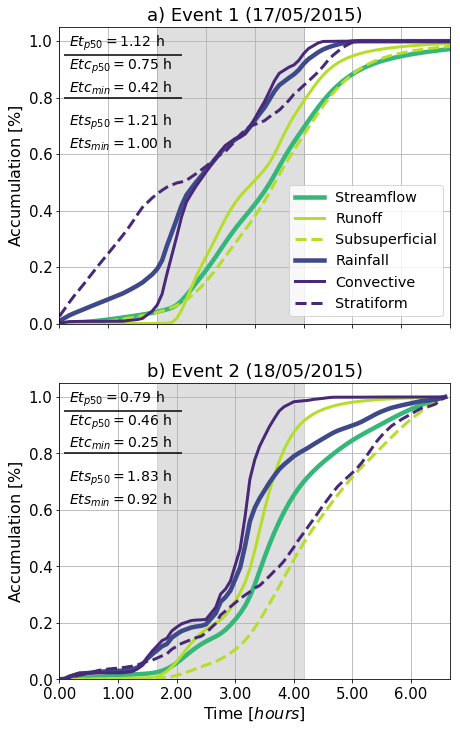
\includegraphics[width=8.3cm]{Figures/Rain_Streamflow_Elapsed.png}
%DIFDELCMD <  %%%
%DIFDELCMD < \caption{%
{%DIFAUXCMD
\DIFdelFL{Accumulated rainfall and streamflow for a)  Event 1 and b) Event 2. The accumulation is expressed in percentage respect to the total value in each case. Median elapsed time and minimum elapsed time () are estimated between total ($Et_{p50}$, $Et_{min}$), convective ($Etc_{p50}$, $Etc_{min}$), and stratiform ($Ets_{p50}$, $Ets_{min}$) rainfall and the runoff portion of the streamflow.  Gray bands correspond to the periods for elapsed time estimation.}}
    %DIFAUXCMD
%DIFDELCMD < \label{fig:lluviaElapsedCaudal}
%DIFDELCMD < \end{figure}
%DIFDELCMD < 

%DIFDELCMD < %%%
\DIFdel{As mentioned before, average rainfall accumulation over the basin for Events 1 and 2 is 47$mm$ and 38$mm$, respectively}\DIFdelend \DIFaddbegin \DIFadd{precipitation during each of the events}\DIFaddend . During Event 1\DIFdelbegin \DIFdel{(2), convective (stratiform) average accumulations are 28 (23) and 17 (14) $mm$, respectively (Figure \ref{fig:RainAcumByReach}a and b). The maximum rainfall intensities are relatively similar with 150$mm/h$ and 180$mm/h$ for Events 1 and 2, respectively.  Despite this, Event 1 does not trigger a flash flood event. The overall evidence suggests that the discriminating factor between both events does not lie in the portions of convective or stratiform rainfall but rather in their spatial distribution. }\DIFdelend \DIFaddbegin \DIFadd{, the convective precipitation occurred near the end of the event, explaining the delayed peak discharge time (see Figure \ref{fig:separacionLluvia}). }\DIFaddend \\ 

\DIFdelbegin \DIFdel{Figures \ref{fig:RainAcumByReach}a and b, and Figures \ref{fig:RainAcumByReach}c and d show the convective and stratiform cumulative rainfall, and the spatially-averaged convective and stratiform rainfall, both as a function of sub-basin reach, respectively.  Figures \ref{fig:RainAcumByReach}a and b show that while  Event 1 exhibit similar convective and stratiform rainfall accumulation for different watershed scales, Event 2 shows a more significant cumulative contribution of convective rainfall than of stratiform precipitation. Convective rainfall tends to cover less area, and at the same timepresent a spatio-temporal erratic behavior \mbox{%DIFAUXCMD
\citep{Steiner1995, Houze1989}}\hspace{0pt}%DIFAUXCMD
. Figures \ref{fig:RainAcumByReach}c and d provide evidence that convective rainfall present higher variations at small sub-basins than for a larger-order basin. During Event 2, convective accumulation reaches higher values for small and medium sub-basins.   Convective rainfall occurrence at the upper sub-basins has significant implications due to geomorphological conditions associated to zero-order sub-basins \mbox{%DIFAUXCMD
\citep{Sidle2018}}\hspace{0pt}%DIFAUXCMD
. Figure \ref{fig:PearsonCorr} presents Pearson correlations coefficients between the convective and stratiform hydrograph portions and the runoff and subsurface flow. According to this, convective and stratiform rainfall exhibit a weaker relationship with the flow characteristics at small scales (under 5$km^2$).  This is likely to be associated with increasing variability of rainfall and hydrograph formation at small scales \mbox{%DIFAUXCMD
\citep{Ayalew2014}}\hspace{0pt}%DIFAUXCMD
.  Correlations tend to grow with increasing  area, indicating stabilization of the hydrograph formation.  Additionally,  subsurface flow presents higher correlations during Event 1, while correlations with runoff are higher for Event 2, highlighting the most important process in each case.  The relevance of subsurface flow is likely due to the rainfall characteristics during  Event 1, with homogeneous rainfall intensity and high rate of basin recharge (see Figure \ref{fig:SimStreamflow}b).On the other hand, saturation processes and a wet soil profile explain the observed higher correlations during Event 2. }\DIFdelend \DIFaddbegin \DIFadd{According to Figure \ref{fig:lluviaElapsedCaudal}b, the accumulations of streamflow runoff and convective rainfall become similar with the increase in time. Additionally, the runoff has a lag and shows signs of attenuation of the convective signal.  However, this description only applies for the runoff portion, since the evolution is different when we consider the total simulated streamflow.}\DIFaddend \\


\begin{figure}[t]
\centering
 \DIFdelbeginFL %DIFDELCMD < 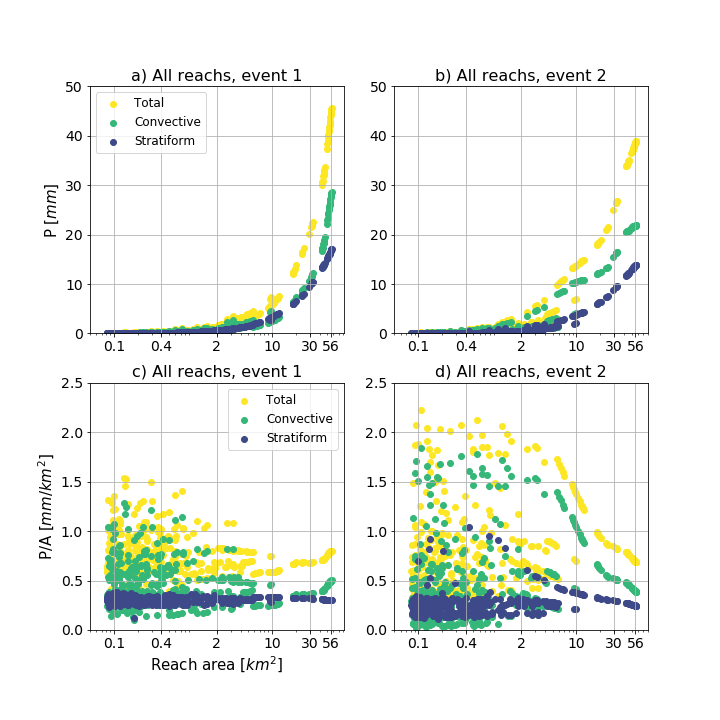
\includegraphics[width=8.3cm]{Figures/RainAcum_by_reach.png}
%DIFDELCMD <  %%%
\DIFdelendFL \DIFaddbeginFL 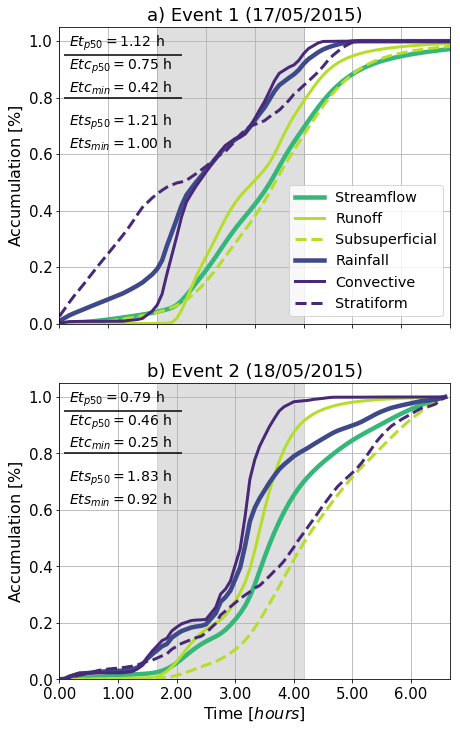
\includegraphics[width=8.3cm]{Figures/Rain_Streamflow_Elapsed.png}
 \DIFaddendFL \caption{\DIFdelbeginFL \DIFdelFL{Cumulative }\DIFdelendFL \DIFaddbeginFL \DIFaddFL{Accumulated }\DIFaddendFL rainfall \DIFdelbeginFL \DIFdelFL{versus the area at each reach of the basin }\DIFdelendFL \DIFaddbeginFL \DIFaddFL{and streamflow }\DIFaddendFL for a) Event 1 and b) \DIFaddbeginFL \DIFaddFL{Event }\DIFaddendFL 2. \DIFdelbeginFL \DIFdelFL{Panels c}\DIFdelendFL \DIFaddbeginFL \DIFaddFL{The accumulation is expressed in percentage with respect to the total value in each case. The median elapsed time and minimum elapsed time () are estimated between total ($Et_{p50}$, $Et_{min}$}\DIFaddendFL )\DIFaddbeginFL \DIFaddFL{, convective ($Etc_{p50}$, $Etc_{min}$), }\DIFaddendFL and \DIFdelbeginFL \DIFdelFL{d}\DIFdelendFL \DIFaddbeginFL \DIFaddFL{stratiform ($Ets_{p50}$, $Ets_{min}$}\DIFaddendFL ) \DIFdelbeginFL \DIFdelFL{show the average }\DIFdelendFL rainfall \DIFdelbeginFL \DIFdelFL{versus }\DIFdelendFL \DIFaddbeginFL \DIFaddFL{and }\DIFaddendFL the \DIFdelbeginFL \DIFdelFL{area at each reach }\DIFdelendFL \DIFaddbeginFL \DIFaddFL{runoff portion }\DIFaddendFL of the \DIFdelbeginFL \DIFdelFL{basin}\DIFdelendFL \DIFaddbeginFL \DIFaddFL{streamflow}\DIFaddendFL . \DIFdelbeginFL \DIFdelFL{Yellow dots }\DIFdelendFL \DIFaddbeginFL \DIFaddFL{Gray bands }\DIFaddendFL correspond to the \DIFdelbeginFL \DIFdelFL{total, green dots to convective and blue dots to stratiform rainfall. All panels use a logarithmic scale }\DIFdelendFL \DIFaddbeginFL \DIFaddFL{periods }\DIFaddendFL for \DIFdelbeginFL \DIFdelFL{the basin area}\DIFdelendFL \DIFaddbeginFL \DIFaddFL{elapsed time estimation}\DIFaddendFL .}
    \DIFdelbeginFL %DIFDELCMD < \label{fig:RainAcumByReach}
%DIFDELCMD < %%%
\DIFdelendFL \DIFaddbeginFL \label{fig:lluviaElapsedCaudal}
\DIFaddendFL \end{figure}


\DIFdelbegin %DIFDELCMD < \begin{figure}[t]
%DIFDELCMD < \centering
%DIFDELCMD <  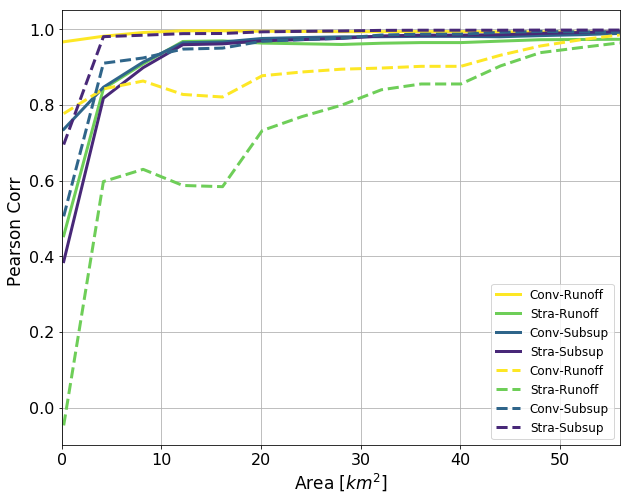
\includegraphics[width=8.3cm]{Figures/CorrPearson_TipoRain_Fluxes.png}
%DIFDELCMD <  %%%
%DIFDELCMD < \caption{%
{%DIFAUXCMD
\DIFdelFL{Pearson correlations among convective and stratiform portions of the rainfall and runoff and subsurface flow for different reach areas. Dashed lines correspond to Event 1 and continuous lines Event 2.}}
    %DIFAUXCMD
%DIFDELCMD < \label{fig:PearsonCorr}
%DIFDELCMD < \end{figure}
%DIFDELCMD < %%%
\DIFdelend %DIF > Figures \ref{fig:RainAcumByReach}a and b, and Figures \ref{fig:RainAcumByReach}c and d show the convective and stratiform cumulative rainfall, and the spatially-averaged convective and stratiform rainfall, both as a function of subbasin reach, respectively.  Figures \ref{fig:RainAcumByReach}a and b show that while  Event 1 exhibit similar convective and stratiform rainfall accumulation for different watershed scales, Event 2 shows a more significant cumulative contribution of convective rainfall than of stratiform precipitation. Convective rainfall tends to cover less area, and at the same time present a spatio-temporal erratic behavior \citep{Steiner1995, Houze1989}. Figures \ref{fig:RainAcumByReach}c and d provide evidence that convective rainfall present higher variations at small subbasins than for a larger-order basin. During Event 2, convective accumulation reaches higher values for small and medium subbasins.   Convective rainfall occurrence at the upper subbasins has significant implications due to geomorphological conditions associated to zero-order subbasins \citep{Sidle2018}. Figure \ref{fig:PearsonCorr} presents Pearson correlations coefficients between the convective and stratiform hydrograph portions and the runoff and subsurface flow. According to this, convective and stratiform rainfall exhibit a weaker relationship with the flow characteristics at small scales (under 5$km^2$).  This is likely to be associated with increasing variability of rainfall and hydrograph formation at small scales \citep{Ayalew2014}.  Correlations tend to grow with increasing  area, indicating stabilization of the hydrograph formation. Additionally,  subsurface flow presents higher correlations during Event 1, while correlations with runoff are higher for Event 2, highlighting the most important process in each case.  The relevance of subsurface flow is likely due to the rainfall characteristics during  Event 1, with homogeneous rainfall intensity and high rate of basin recharge (see Figure \ref{fig:SimStreamflow}b).  On the other hand, saturation processes and a wet soil profile explain the observed higher correlations during Event 2. \\

\DIFdelbegin \subsection{\DIFdel{Landslide and flood simulations}}
%DIFAUXCMD
\addtocounter{subsection}{-1}%DIFAUXCMD
\DIFdelend %DIF > \begin{figure}[t]
%DIF > \centering
%DIF >  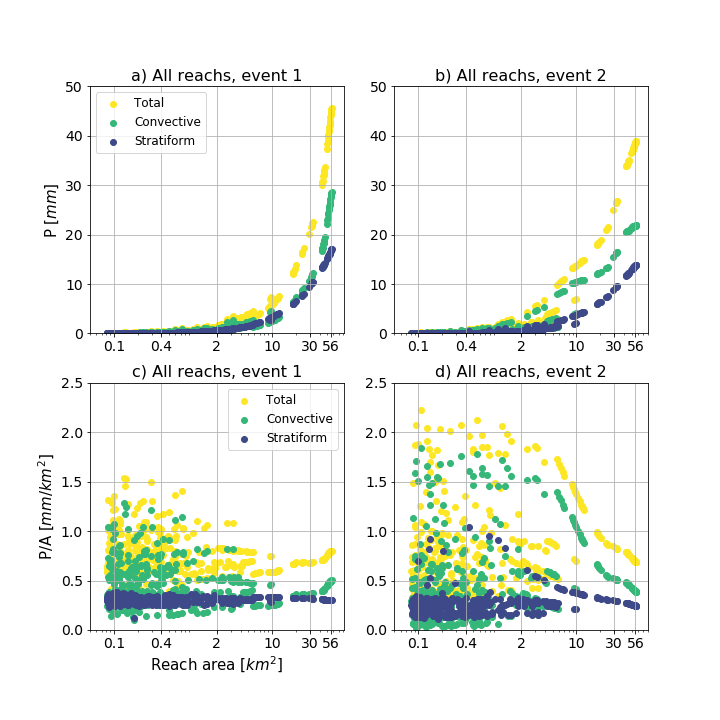
\includegraphics[width=8.3cm]{Figures/RainAcum_by_reach.png}
%DIF >  \caption{Cumulative rainfall versus the area at each reach of the basin for a) Event 1 and b) 2. Panels c) and d) show the average rainfall versus the area at each reach of the basin. Yellow dots correspond to the total, green dots to convective and blue dots to stratiform rainfall. All panels use a logarithmic scale for the basin area.}
 %DIF >    \label{fig:RainAcumByReach}
%DIF > \end{figure}

\DIFdelbegin \DIFdel{In addition to the hydrological simulation, associated hazards such as floods and landslides are also modeled and discussed in this study. The landslides model as described in the previous section requires additional information including soil depth $Z$, cohesion $C'$, friction angle $\phi$ and specific weight $\gamma$.  According to the  description by  \mbox{%DIFAUXCMD
\citet{Osorio2008}}\hspace{0pt}%DIFAUXCMD
, illustrating a clay-slime soil,   $C'$  is  assumed equal to 4$KN$, $\phi$ to 30$^0$ and $\gamma$ to 18; $Z$ vary with slope according to Table \ref{tab:suelos}. }%DIFDELCMD < \\
%DIFDELCMD < %%%
\DIFdelend %DIF > \begin{figure}[t]
%DIF > \centering
%DIF >  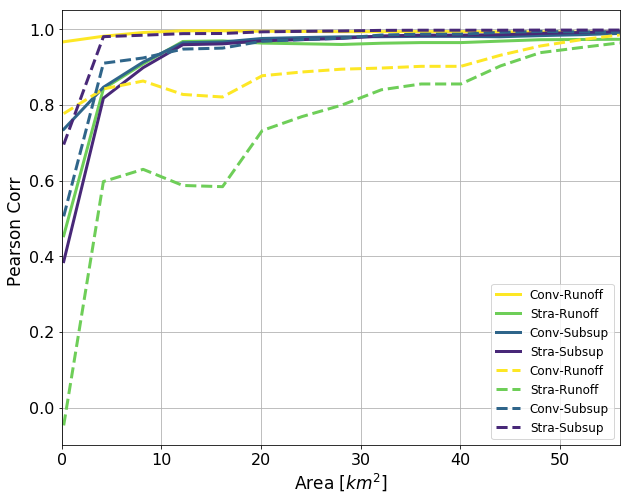
\includegraphics[width=8.3cm]{Figures/CorrPearson_TipoRain_Fluxes.png}
%DIF >  \caption{Pearson correlations among convective and stratiform portions of the rainfall and runoff and subsurface flow for %different reach areas. Dashed lines correspond to Event 1 and continuous lines Event 2.}
 %DIF >    \label{fig:PearsonCorr}
%DIF > \end{figure}
\DIFaddbegin 


\subsection{\DIFadd{Landslide and flood simulations}}
\DIFaddend 

Figure \ref{fig:SlidesComparison}a presents the observed landslides triggered by Event 2  based on aerial photos and satellite images (Landsat/Copernicus \DIFdelbegin \DIFdel{, }\DIFdelend and Google) taken before and after the flash flood.  Figure \ref{fig:SlidesComparison}b shows, by hills, the map of total unstable cells during the simulation period, and Figure \ref{fig:SlidesComparison}c shows the time series of the number of simulated unstable cells during Event 2 (continuous purple line) and the mean rainfall over the basin (inverse axes, blue line). Calibration of the landslide model was performed by finding the maximum overlap between simulated and observed unstable and stable cells, and at the same time reducing the overall number of false positives and false negatives. It is important to note that the calibration strategy is not a cell-by-cell modification of the parameters involved but rather a basin-wide modification of soil properties. A sensitivity analysis of soil parameters is carried out by making small variations of the variables within specified intervals: $\phi$ between 25 and 32, $\gamma$ between 17 and 19,  $C'$ between 3.5 and 4.2, and $Z$ between 0.1 and 3 $m$. The sensitivity analysis suggests that slight variations in the parameter in $Z$ produce significant changes in the \DIFdelbegin \DIFdel{modeled landslides, resulting in an }\DIFdelend \DIFaddbegin \DIFadd{results, with }\DIFaddend overestimation of the number of unstable cells \DIFdelbegin \DIFdel{, }\DIFdelend or no unstable cells at all. Following Table \ref{tab:suelos}, the average soil depth in the basin is only 0.3 m, a value that corresponds to underestimation according to the inspections during field visits. For this reason, the results presented in Figure \ref{fig:SlidesComparison} use a  $Z$ map scaled by a calibration factor of 3.5, preserving the spatial dependence on the slope \DIFdelbegin \DIFdel{, }\DIFdelend but achieving a more realistic soil depth and better spatial distribution of \DIFaddbegin \DIFadd{a }\DIFaddend landslide occurrence.\\ 


\begin{figure}[t!]
\centering
 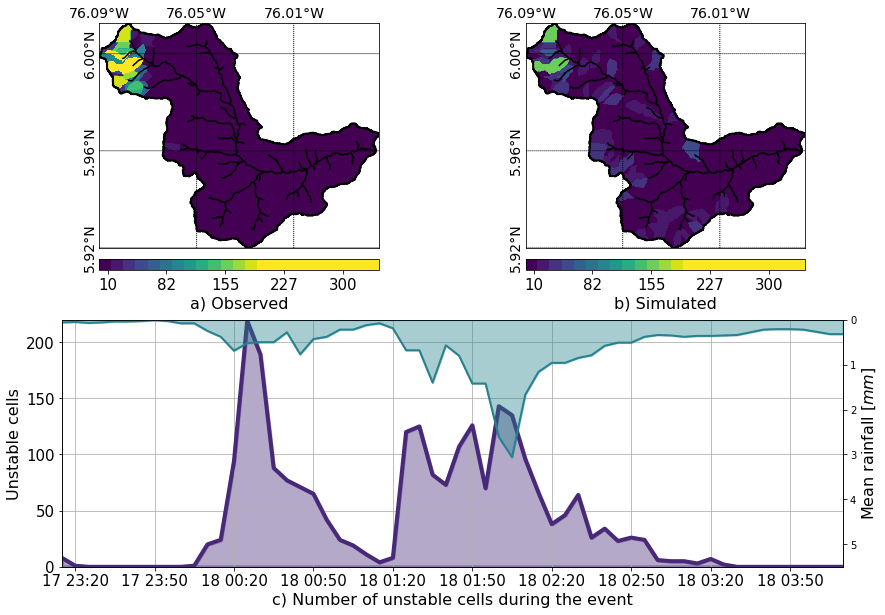
\includegraphics[width=12cm]{Figures/Slides_byHills.png}
 \caption{a) Observed landslides triggered by Events 1 and 2. The figure is based on aerial photos and satellite images (Landsat/Copernicus, and images available on Google) taken before and after the flash flood event. b) Map of total unstable cells during the simulation period. c) Time series of \DIFaddbeginFL \DIFaddFL{the }\DIFaddendFL number of simulated unstable cells during Event 2 (continuous purple line) and mean rainfall over the basin (inverse axes, blue line).}
    \label{fig:SlidesComparison}
\end{figure}

The model represents \DIFdelbegin \DIFdel{considerably well }\DIFdelend the spatial distribution of the areas that are prone to trigger shallow landslides during Event 2 \DIFaddbegin \DIFadd{reasonably well, especially in the upper part of the basin}\DIFaddend , showing a significant density of unstable cells in the hills where slides took place. \DIFdelbegin \DIFdel{However, despite the calibration efforts, the total number of unstable cells is relatively low compared to observations. It is important to note that there was no spatial calibration in order to obtain the right location of the landslides. The calibration only includes the change of the soil depth using a single scalar, constant for the entire basin, in order to maximize the number matching observed and simulated slides. In other words, there is just one single basin-wide parameter modified, and not an independent modification of the parameter for every pixel in order to obtain the right distribution.  This }\DIFdelend \DIFaddbegin \DIFadd{This result }\DIFaddend is important because in that sense, it serves to \DIFdelbegin \DIFdel{check }\DIFdelend \DIFaddbegin \DIFadd{verify }\DIFaddend the capability of the model to estimate risk areas only considering topography and rainfall data. \DIFaddbegin \DIFadd{On the other hand, there are some false positives in the middle of the basin, which could be related to the poor description of the soils. The landslide model has been used in a nearby watershed with similar characteristics, but with high-quality distributed information \mbox{%DIFAUXCMD
\citep{Aristizabal2016}}\hspace{0pt}%DIFAUXCMD
. In that case, the model shows a better performance, which highlights the relevance of the input data. }\DIFaddend A pinpoint localization of the unstable cells is still considered a hard task\DIFaddbegin \DIFadd{, }\DIFaddend in part due to the small temporal and spatial scale at which landslide processes take place \citep{Aristizabal2016, Dhakal2004, Wu1995}. \DIFdelbegin \DIFdel{Additionally,  the lack of detailed soil information increases the simulation uncertainty. }\DIFdelend Notwithstanding the difficulties, the results suggest that the model simulations could have been used and should be used in the future for early detection and warning to improve both \DIFdelbegin \DIFdel{short }\DIFdelend \DIFaddbegin \DIFadd{short- }\DIFaddend and long-term risk reduction strategies.\\

Figure \ref{fig:SimFloodSpots} shows the identification of the flood spots at the peak of Event 2 (May \DIFdelbegin \DIFdel{18th}\DIFdelend \DIFaddbegin \DIFadd{18}\DIFaddend , 2015, 2:00 a.m.) as simulated using \DIFdelbegin \DIFdel{HydroFlah}\DIFdelend \DIFaddbegin \DIFadd{HydroFlash}\DIFaddend . Figures \ref{fig:SimFloodSpots}b to f present a \DIFdelbegin \DIFdel{detail }\DIFdelend \DIFaddbegin \DIFadd{detailed }\DIFaddend view of the results from the outlet of the basin to the upper region. Cases presented in Figures \ref{fig:SimFloodSpots}e and f exhibit a satisfactory agreement with observed flood spots (blue shadow).  Cases in Figures \ref{fig:SimFloodSpots}c and d also show a good approximation, but with minor spatial shifts in some sections. The largest spatial differences are observed in Figures \ref{fig:SimFloodSpots}b. At the entrance of the urban zone, the model overestimates the flood spots. The model results indicate that 11\% of flood spots \DIFdelbegin \DIFdel{happen }\DIFdelend \DIFaddbegin \DIFadd{occur }\DIFaddend at elements of order 1 and 2, and \DIFdelbegin \DIFdel{, }\DIFdelend 18, 38 and 32\% \DIFdelbegin \DIFdel{happen }\DIFdelend \DIFaddbegin \DIFadd{occur }\DIFaddend at orders 3, 4 and 5, respectively.  \DIFdelbegin \DIFdel{This also highlights }\DIFdelend \DIFaddbegin \DIFadd{Table \ref{tab:flash}  summarizes the described percentages and the total length of each order. These results also highlight }\DIFaddend a coherent geomorphological representation of the flooded channels and hills \DIFdelbegin \DIFdel{with }\DIFdelend \DIFaddbegin \DIFadd{relative to }\DIFaddend the order.\\   


\DIFaddbegin \begin{table}[!h]
\centering
  \caption{\DIFaddFL{Channels and flooded cells percentages summary.  $Sh_0$ and $Ss_0$ correspond to the mean hill and stream slope, respectively. $L$ corresponds to the total channel length. F Spots and S spots correspond to the flooded and slides percentages, respectively.}}
\begin{tabular}{lccccr}
\hline
\DIFaddFL{Order }& \DIFaddFL{$Sh_0$ $[\%]$ }& \DIFaddFL{$Ss_0$  $[\%]$ }& \DIFaddFL{$L$ $[km]$ }& \DIFaddFL{F Spots }& \DIFaddFL{Ss Spots }\\
\hline
\DIFaddFL{1 }& \DIFaddFL{60 }& \DIFaddFL{37 }& \DIFaddFL{59 }& \DIFaddFL{5 }& \DIFaddFL{64.5 }\\
\DIFaddFL{2 }& \DIFaddFL{57 }& \DIFaddFL{27 }& \DIFaddFL{26 }& \DIFaddFL{6 }& \DIFaddFL{26.3}\\
\DIFaddFL{3 }& \DIFaddFL{49 }& \DIFaddFL{13 }& \DIFaddFL{16 }& \DIFaddFL{18.5 }& \DIFaddFL{5.5}\\
\DIFaddFL{4 }& \DIFaddFL{43 }& \DIFaddFL{9 }& \DIFaddFL{10 }& \DIFaddFL{38.5 }& \DIFaddFL{3.6}\\
\DIFaddFL{5 }& \DIFaddFL{42 }& \DIFaddFL{6 }& \DIFaddFL{6 }& \DIFaddFL{32 }& \DIFaddFL{0.05}\\
\hline
\textbf{\DIFaddFL{Mean/total}} & \DIFaddFL{50 }& \DIFaddFL{18 }& \DIFaddFL{117 }& \DIFaddFL{100 }& \DIFaddFL{100 }\\
\hline
\end{tabular}
\label{tab:flash}
\end{table}


\DIFaddend \begin{figure}[t!]
\centering
 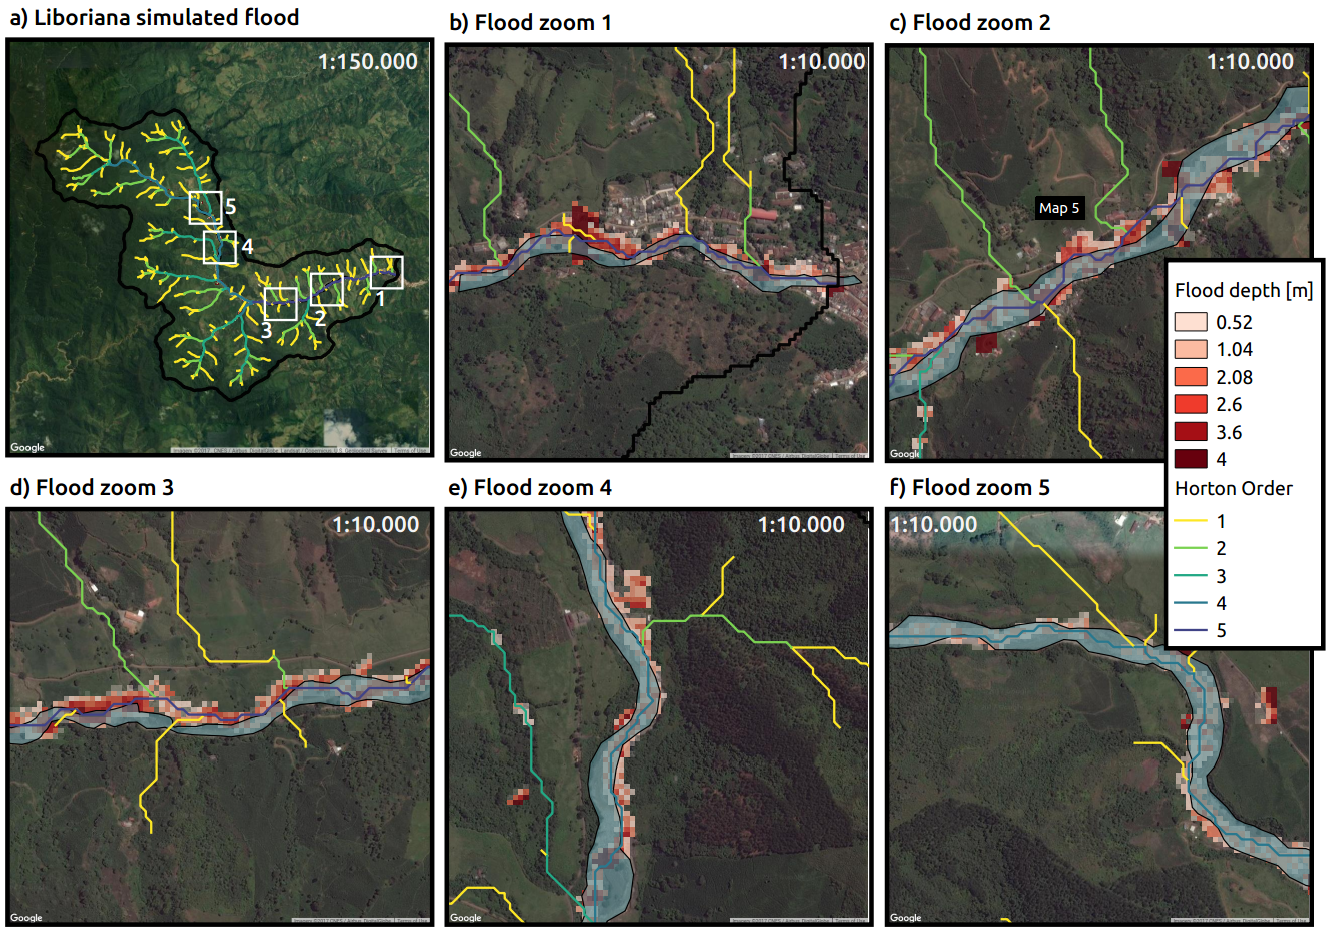
\includegraphics[width=12cm]{Figures/Manchas2.png}
 \caption{Simulated flood spot at the peak of Event 2 in different locations. a) Basin drainage network. White squares correspond to regions of interest highlighted in panes b) to f). The colors of the streams correspond to the Strahler order of the network. b) Zoom at the outlet of the basin, where an important portion of the human and infrastructure \DIFdelbeginFL \DIFdelFL{loses }\DIFdelendFL \DIFaddbeginFL \DIFaddFL{losses }\DIFaddendFL took place. c) Zoom at La Margarita settlement also affected by the flash flood. d) to f) Zoom at key locations along the principal stream. Observed flood spots are shown in blue polygons and model flood spots in red to white grids.}
    \label{fig:SimFloodSpots}
\end{figure}

%\vspace{5cm}
%%-----------------------------------------------------------
%%-----------------------------------------------------------
%Discussion
%%-----------------------------------------------------------
%%-----------------------------------------------------------

\section{Discussion}
\label{sec:discussion}

\DIFdelbegin \DIFdel{During }\DIFdelend \DIFaddbegin \DIFadd{On }\DIFaddend the morning of May \DIFdelbegin \DIFdel{18th of }\DIFdelend \DIFaddbegin \DIFadd{18, }\DIFaddend 2015, a flash flood occurred in the steep La Liboriana basin, in the municipality of Salgar, Department of Antioquia, Colombia, leaving more than 100 human casualties, 535 houses destroyed, and significant infrastructure loses.  Due to the lack of local information of soil type, land use and real-time hydrometeorological data, \DIFaddbegin \DIFadd{the }\DIFaddend La Liboriana case implies a challenge for flash flood prediction, modeling and, consequently, risk management. The present paper introduces a hydrologic model-based approach and an integral graphical analysis tool (an integrated spatiotemporal analysis of rainfall evolution, together with soil storages in the basin) \DIFdelbegin \DIFdel{,  not only }\DIFdelend \DIFaddbegin \DIFadd{for the following purposes: 1) }\DIFaddend to simulate and understand \DIFdelbegin \DIFdel{all the  relevant }\DIFdelend \DIFaddbegin \DIFadd{the  }\DIFaddend soil-rainfall-discharge processes that led to the 2015 Salgar flash flood\DIFdelbegin \DIFdel{while assessing the associated natural hazards, but also }\DIFdelend \DIFaddbegin \DIFadd{, and 2) }\DIFaddend to propose it as a radar QPE-based \DIFaddbegin \DIFadd{and modeling-based }\DIFaddend landslide and flash flood guidance low-cost tool for basins with scarce data and regions with limited resources.\\

The methodology implies the development of a distributed hydrologic model with the capabilities of tracking independently convective and stratiform precipitation within the model\DIFaddbegin \DIFadd{, }\DIFaddend as well as keeping track of the runoff and subsurface portions of the streamflow,  \DIFdelbegin \DIFdel{coupling }\DIFdelend \DIFaddbegin \DIFadd{coupled with }\DIFaddend a shallow landslide submodel and \DIFaddbegin \DIFadd{HydroFlash, }\DIFaddend a one-dimensional flash flood scheme\DIFdelbegin \DIFdel{(HydroFlash)}\DIFdelend .  The model proposed here indeed allows studying the different hydrological processes relevant to flash flood and landslide occurrence by using different simulation resources, serving as the basis for a better understanding of the overall basin response. This \DIFdelbegin \DIFdel{overall }\DIFdelend approach helps to \DIFdelbegin \DIFdel{isolate flood generating }\DIFdelend \DIFaddbegin \DIFadd{examine flood-generating }\DIFaddend mechanisms or causative factors both in time and \DIFdelbegin \DIFdel{also }\DIFdelend in space, focusing on the important physical processes \DIFdelbegin \DIFdel{and not only on statistics }\DIFdelend \citep{klemes1993, Merz2003}. It is hoped that knowledge improvement leads to the anticipation of \DIFdelbegin \DIFdel{the }\DIFdelend warning and response by risk management entities. \\

The evolution of the simulation of Events 1 and 2 show evidence of remarkable behavioral differences. During Event 1\DIFaddbegin \DIFadd{, }\DIFaddend both gravitational and capillary tanks are filled along and across the basin as a result of the quasi-homogeneous rainfall spatial distribution \DIFaddbegin \DIFadd{\mbox{%DIFAUXCMD
\citep{Zoccatelli2011}}\hspace{0pt}%DIFAUXCMD
}\DIFaddend . The return flow is low, and most of the runoff occurs within the first 20 groups (40\% of the watershed closest to the outlet). In the period between both events, there is a recession in the capillary and gravitational storages in the entire basin. Capillary storage decays considerably slower than gravitational storage. During Event 2, the flash flood triggering event, the first convective core saturates both capillary and gravitational storages in the upper part of the basin and generates both return flow and significant runoff. Due to soil saturation, the second convective core results mainly in surface runoff. During this event, \DIFdelbegin \DIFdel{runoff is generated the lower part of the basin while }\DIFdelend extreme runoff rates are evident in the upper part of the basin, collocated with the steeper slopes. On the other hand, subsurface flow is more important in magnitude than runoff describing Event 1, while runoff is more relevant for Event 2. The precedent storage and the presence of thunderstorm training profoundly condition the streamflow during Event 2. The overall evidence suggests that precedent capillary moisture in the basin plays an essential role in modulating river discharge. This behavior could be linked to the temporal occurrence and relative importance and timing of stratiform and convective formations previously described. \\


While convective and stratiform partitioning could influence the runoff and subsurface flow separation, the spatial distribution of rainfall relative to watershed network morphometry structure impose a condition on the hydrological response of the basin \DIFaddbegin \DIFadd{\mbox{%DIFAUXCMD
\citep{Douinot2016}}\hspace{0pt}%DIFAUXCMD
}\DIFaddend . In other words, hydrograph formation is \DIFdelbegin \DIFdel{not only determined }\DIFdelend \DIFaddbegin \DIFadd{determined  not only }\DIFaddend by the rainfall accumulation or maximum intensity \DIFdelbegin \DIFdel{, }\DIFdelend but also by its spatial structure \DIFaddbegin \DIFadd{\mbox{%DIFAUXCMD
\citep{Zoccatelli2011,Douinot2016}}\hspace{0pt}%DIFAUXCMD
. As mentioned before, average rainfall accumulation over the basin for Events 1 and 2 is 47$mm$ and 38$mm$, respectively. During  Event 1 (2), convective (stratiform) average accumulations are 28 (23) and 17 (14) $mm$, respectively.  The maximum rainfall intensities are relatively similar with 150$mm/h$ and 180$mm/h$ for Events 1 and 2, respectively, but the location was significantly different.  Convective rainfall occurrence at the upper subbasins has significant implications due to geomorphological conditions associated to zero-order subbasins \mbox{%DIFAUXCMD
\citep{Sidle2018}}\hspace{0pt}%DIFAUXCMD
. Additionally, when we compare Events 1 and 2, there is an interplay between the rain spatial structure and the soil storage capacity. During Event 1, there is almost no saturation, hence runoff production is low, while Event 2 is influenced by the pre-event water and the occurrence of multiple convective systems over the same region}\DIFaddend .  The structure of the rainfall associated with \DIFaddbegin \DIFadd{the }\DIFaddend La Liboriana event \DIFaddbegin \DIFadd{and its interaction with the soils }\DIFaddend highlights the need to consider in more detail the role of orographic rainfall intensification in practical applications such as early warning systems.  Evidence suggests the spatial structure of the rainfall is at least as important as the geomorphological features of the basin \DIFaddbegin \DIFadd{in }\DIFaddend regulating the generation of flash flood events.\\

An integrated spatiotemporal analysis of rainfall evolution, together with soil storages in the basin\DIFaddbegin \DIFadd{, }\DIFaddend is necessary to study the relevance of antecedent conditions and precipitation type, intensity, and location in the generation of flash flood events.  Event 1 increased the overall soil moisture with an associated decrease \DIFdelbegin \DIFdel{on infiltration ratessimilar to }\DIFdelend \DIFaddbegin \DIFadd{in infiltration rates, similar to the }\DIFaddend results reported by \DIFdelbegin \DIFdel{\mbox{%DIFAUXCMD
\citet{Penna2011} }\hspace{0pt}%DIFAUXCMD
and \mbox{%DIFAUXCMD
\citet{Zehe2010}}\hspace{0pt}%DIFAUXCMD
}\DIFdelend \DIFaddbegin \DIFadd{\mbox{%DIFAUXCMD
\citet{Marchi2010,Penna2011} }\hspace{0pt}%DIFAUXCMD
and \mbox{%DIFAUXCMD
\citet{Zehe2010}}\hspace{0pt}%DIFAUXCMD
; additionally}\DIFaddend , low infiltration \DIFdelbegin \DIFdel{increase }\DIFdelend \DIFaddbegin \DIFadd{increased the }\DIFaddend runoff rates, \DIFdelbegin \DIFdel{which finally affects }\DIFdelend \DIFaddbegin \DIFadd{ultimately affecting }\DIFaddend the susceptibility of the basin to  flash \DIFdelbegin \DIFdel{floods }\DIFdelend \DIFaddbegin \DIFadd{flood }\DIFaddend occurrence \citep{Wagner1999,Penna2011,Tramblay2012b}. \DIFdelbegin \DIFdel{La Liboriana geomorphological characteristics , corresponding to a steep tropical basin, determine the potential energy that controls water transit velocity.  Water }\DIFdelend \DIFaddbegin \DIFadd{Due to geomorphological characteristics (see Table \ref{tab:flash}), water }\DIFaddend tends to reach faster the channels in \DIFaddbegin \DIFadd{hills of }\DIFaddend order 1 and 2\DIFdelbegin \DIFdel{hills}\DIFdelend , and, at the same time, the sediment production and transport in these hills tend to be larger.  Order 3 \DIFdelbegin \DIFdel{sub-basins }\DIFdelend \DIFaddbegin \DIFadd{subbasins }\DIFaddend most likely act as transport elements, with no important energy losses \DIFdelbegin \DIFdel{. Floods }\DIFdelend \DIFaddbegin \DIFadd{(Table \ref{tab:flash}), and floods }\DIFaddend tend to occur \DIFdelbegin \DIFdel{in }\DIFdelend \DIFaddbegin \DIFadd{at }\DIFaddend order 4 and 5 \DIFdelbegin \DIFdel{sub-basins }\DIFdelend \DIFaddbegin \DIFadd{subbasins }\DIFaddend due to the widening of the channel and slope attenuation.\\

Different authors have focused on trying to understand the general causative factors behind the occurrence of flash floods \DIFdelbegin \DIFdel{finding similar to our results, }\DIFdelend \DIFaddbegin \DIFadd{\mbox{%DIFAUXCMD
\citep{Marchi2010}}\hspace{0pt}%DIFAUXCMD
, finding results similar to ours, with }\DIFaddend a significant role of \DIFdelbegin \DIFdel{basing }\DIFdelend \DIFaddbegin \DIFadd{considering }\DIFaddend geomorphology, orography and local convection. For example, \citet{Lehmann2012}, using a shallow landslide model, finds an important role of the topography and the rainfall conditions. \citet{Turkington2014} shows how intense locally driven convection appears to be the main meteorological trigger for flash occurrence in the French \DIFdelbegin \DIFdel{Alpes}\DIFdelend \DIFaddbegin \DIFadd{Alps}\DIFaddend .\citet{Camarasa2016} shows how rainfall intensity and duration influences the shape of the hydrograph, with intense rainfall shortening the response time of the basin, and large durations increasing the flood peak. In the Mediterranean region, \citet{Boudou2016} states that in addition to the rainfall, geomorphological characteristics and antecedent soil conditions are key in the generation of flash flooding.\\

However useful, the evidence in this work only takes into account two successive events; an analysis of more cases and different spatial scales (different basins) would provide robust conclusions in this direction. It is clear that \DIFdelbegin \DIFdel{it is not conclusive enough to focus }\DIFdelend \DIFaddbegin \DIFadd{focusing }\DIFaddend on a single extreme event, rather than on a spectrum of floods\DIFaddbegin \DIFadd{, is not conclusive enough }\DIFaddend \cite{Merz2003}.  The model simulation results suggest it is imperative to study in depth the long-term link between the relative basin and drainage network orientation and the preferred path of precipitation events and its role in defining the frequency of flash flood occurrence. A better understanding of the network-hills-preferential rainfall advection structure could provide information about basins prone to flash floods when information is scarce.\\



\conclusions[Conclusions]
\label{sec:conclusions}

Extreme rainfall events such as the one that triggered \DIFaddbegin \DIFadd{the }\DIFaddend La Liboriana tragedy frequently take place in Colombia and the entire global tropical belt over ungauged basins, often triggering flash floods and \DIFdelbegin \DIFdel{torrential flows, endangering }\DIFdelend \DIFaddbegin \DIFadd{debris flows, which endanger }\DIFaddend vulnerable communities due to poor long-term planning and lack of functional early warning systems. There is a global need for better knowledge and understanding of the hydrological and meteorological conditions that, combined, lead to the manifestation of \DIFaddbegin \DIFadd{disasters linked to }\DIFaddend natural hazards. Such \DIFaddbegin \DIFadd{an }\DIFaddend understanding must result in useful practical applications that improve risk management practices \DIFdelbegin \DIFdel{saving }\DIFdelend \DIFaddbegin \DIFadd{and thus save }\DIFaddend lives. In the current work, we approach the problem from a hydrological modeling point of view, trying, despite the data limitations and the uncertainty of the results, to shed some light \DIFdelbegin \DIFdel{in }\DIFdelend \DIFaddbegin \DIFadd{on }\DIFaddend the first-order processes that modulate the occurrence of flash floods in the region \DIFaddbegin \DIFadd{of study}\DIFaddend .  \\  

In the case of \DIFaddbegin \DIFadd{the }\DIFaddend La Liboriana flash flood, radar reflectivity fields were available from a C-Band radar operated by the Early Warning System of Medellín and its metropolitan area\DIFaddbegin \DIFadd{, }\DIFaddend as part of a local risk management strategy. While the municipality of Salgar is located far \DIFdelbegin \DIFdel{outside }\DIFdelend \DIFaddbegin \DIFadd{from }\DIFaddend Medellín's metropolitan area, the radar is \DIFdelbegin \DIFdel{about }\DIFdelend \DIFaddbegin \DIFadd{approximately }\DIFaddend 90 km away from Salgar, and the reflectivity retrievals enable the classification of precipitation fields into convective and stratiform areas\DIFaddbegin \DIFadd{, }\DIFaddend using widely accepted methodologies by the meteorological community.  Radar reflectivity \DIFdelbegin \DIFdel{is also }\DIFdelend \DIFaddbegin \DIFadd{also serves as }\DIFaddend a proxy for precipitation\DIFaddbegin \DIFadd{, }\DIFaddend allowing a quantitative estimation of rainfall fields. This estimation was used together with the hydrologic model to assess the different basin-wide processes taking place during the flash flood triggering rainfall event. The limitations of the methodology presented in this work do not allow \DIFdelbegin \DIFdel{to represent }\DIFdelend \DIFaddbegin \DIFadd{representing }\DIFaddend all the detailed small-scale preferential pathways of \DIFaddbegin \DIFadd{the }\DIFaddend water in the watershed, but rather focus on the first-order \DIFdelbegin \DIFdel{approximation }\DIFdelend \DIFaddbegin \DIFadd{processes }\DIFaddend to study the partitioning between runoff vs. subsurface flow. \DIFdelbegin \DIFdel{Also}\DIFdelend \DIFaddbegin \DIFadd{Additionally}\DIFaddend , the model results are used to obtain a conceptual idea about the general processes, but it must be taken into account that the simulations are subject to a calibration process that could lead to erroneous conclusions about the \DIFdelbegin \DIFdel{physical }\DIFdelend \DIFaddbegin \DIFadd{mentioned }\DIFaddend processes. This \DIFaddbegin \DIFadd{consideration }\DIFaddend could be true even \DIFdelbegin \DIFdel{as }\DIFdelend \DIFaddbegin \DIFadd{when }\DIFaddend different steps were taken trying to avoid this situation.  \\

The overall model simulation methodology reproduces \DIFdelbegin \DIFdel{considerably well the magnitude and timing of }\DIFdelend \DIFaddbegin \DIFadd{the estimated magnitude and reported timing of the }\DIFaddend La Liboriana flash flood discharge peak \DIFaddbegin \DIFadd{quite well}\DIFaddend , showing robustness to changes in the most important model parameters\DIFdelbegin \DIFdel{, and reasonably well }\DIFdelend \DIFaddbegin \DIFadd{. Simulation results suggest that the soil storage capacity available before flooding event, impacted not only the flood magnitude itself, but also the response time of the catchment, highlighting the role of soil wetness distribution within the basin. The model also reproduces }\DIFaddend the areas of regional \DIFdelbegin \DIFdel{land-slide }\DIFdelend \DIFaddbegin \DIFadd{landslide }\DIFaddend occurrence and flood \DIFdelbegin \DIFdel{spots location. Model }\DIFdelend \DIFaddbegin \DIFadd{spot locations satisfactorily. The model }\DIFaddend simulation results indicate that the \DIFdelbegin \DIFdel{flash-flood }\DIFdelend \DIFaddbegin \DIFadd{flash flood }\DIFaddend and the regional \DIFdelbegin \DIFdel{land-slide }\DIFdelend \DIFaddbegin \DIFadd{landslide }\DIFaddend features were strongly influenced by the observed antecedent rainfall associated with a \DIFdelbegin \DIFdel{northeasterly }\DIFdelend \DIFaddbegin \DIFadd{northwesterly }\DIFaddend stratiform event that recharged the gravitational and capillary storages in the entire basin. The \DIFdelbegin \DIFdel{hydrologic }\DIFdelend \DIFaddbegin \DIFadd{hydrological model }\DIFaddend simulation shows that the antecedent event set wet conditions in the entire basin before the occurrence of the flash flood event, governing the streamflow during the latter.  \DIFdelbegin \DIFdel{Results }\DIFdelend \DIFaddbegin \DIFadd{The results }\DIFaddend of the model simulation also suggest that the first of the two successive convective cores (\DIFdelbegin \DIFdel{thunderstorm training }\DIFdelend \DIFaddbegin \DIFadd{training convective elements}\DIFaddend ) over the same region during the second precipitation event (the flash flood event) saturated both capillary and gravitational storages in the upper part of the basin and generated both return flow and significant runoff. The second convective core resulted mainly in surface runoff spatially collocated with the steeper slopes, generating the kinetic energy needed to produce \DIFaddbegin \DIFadd{the }\DIFaddend La Liboriana flash flood. \DIFdelbegin \DIFdel{Overall }\DIFdelend \DIFaddbegin \DIFadd{The overall }\DIFaddend results also show a good agreement between the simulated flood spots and the observed ones\DIFdelbegin \DIFdel{; this in spite of }\DIFdelend \DIFaddbegin \DIFadd{, despite }\DIFaddend the limitations imposed by the resolution of the DEM used for extracting \DIFdelbegin \DIFdel{cross sections, }\DIFdelend \DIFaddbegin \DIFadd{cross-sections }\DIFaddend and the model oversimplifications. \\

\DIFaddbegin \DIFadd{Results of the landslide submodel and HydroFlash, while satisfactory, are far from perfect, showing significant differences compared to observations when compared in the  detail. The evidence suggests, by and large, that most of the observed differences are mainly due to the lack of higher spatial resolution DEM, in the case of HydroFlash, and due to the lack of a detailed soil dataset, in the case of the landslide submodel. However, there is also is considerable room for improvement in both submodels, including a better representation of non-Newtonian hydraulic processes in HydroFlash, and a direct link between landslides and flood spots following, for example, a similar strategy to the one presented in the STEP-TRAMM model \mbox{%DIFAUXCMD
\citep{Fan2017a}}\hspace{0pt}%DIFAUXCMD
.}\\

\DIFaddend Considering all the shortcomings and generalizations, the described model-based approach is potentially useful to assess \DIFdelbegin \DIFdel{flood generating }\DIFdelend \DIFaddbegin \DIFadd{flood-generating }\DIFaddend mechanisms and as a tool for policy-makers, not only for short-term decisions in the context of an early warning system but also as a planning resource for long-term risk management. \DIFdelbegin \DIFdel{While several improvements need to be implemented, including a better representation of hydraulic parameters,  and a direct link between landslides and flood spots similar to the strategy presented in the STEP-TRAMM model \mbox{%DIFAUXCMD
\citep{Fan2017a}}\hspace{0pt}%DIFAUXCMD
, the }\DIFdelend \DIFaddbegin \DIFadd{The }\DIFaddend results suggest it is possible to use low-cost methodologies such as the one introduced here as a risk management tool in countries and regions with scarce resources.\\




%DIF <  \appendix
%DIF <  \section{}    %% Appendix A
\DIFdelbegin %DIFDELCMD < 

%DIFDELCMD < %%%
%DIF <  \subsection{}                               %% Appendix A1, A2, etc.
%DIFDELCMD < 

%DIFDELCMD < %%%
\DIFdelend \section{\DIFdelbegin \DIFdel{Acknowledgements}\DIFdelend \DIFaddbegin \DIFadd{Acknowledgments}\DIFaddend }
This work was supported by SIATA (Sistema de Alerta Temprana de Medellín y el Valle de Aburrá)  funds provided by Area Metropolitana del Valle de Aburrá (AMVA), Municipio de Medellín, Grupo EPM, and ISAGEN under the Research and Technology Contract CD511, 2017.  Universidad Nacional de Colombia partly funded Nicolás Velásquez under the Facultad de Minas graduate scholarship program. Both authors would like to thank anonymous reviewer #1 for the detailed and insightful comments that helped to clarify and highlight the message of this work.  Both authors also thank Dr. Eric Gaume, reviewer #2, for his thoughtful comments.\\

For the technically inclined reader, the hydrologic model and \DIFdelbegin \DIFdel{sub-models }\DIFdelend \DIFaddbegin \DIFadd{submodels }\DIFaddend are written in Fortran 90, and the interface to the model, pre-process, and post-process tools are in \DIFdelbegin \DIFdel{python }\DIFdelend \DIFaddbegin \DIFadd{Python }\DIFaddend 2.7. The Fortran code is warped to \DIFdelbegin \DIFdel{python }\DIFdelend \DIFaddbegin \DIFadd{Python }\DIFaddend using \textbf{f2py} \citep{Peterson2009}\DIFaddbegin \DIFadd{, }\DIFaddend and it is publicly available under the Watershed \DIFdelbegin \DIFdel{Modelling }\DIFdelend \DIFaddbegin \DIFadd{Modeling }\DIFaddend Framework \textbf{WMF} in a web repository (\href{https://github.com/nicolas998/WMF.git}{\textbf{GitHub}}). \\
\DIFaddbegin 

\appendix
\renewcommand\thefigure{\thesection.\arabic{figure}}    
\section{\DIFadd{Figures}}
\setcounter{figure}{0}    
\begin{figure}[t]
\centering
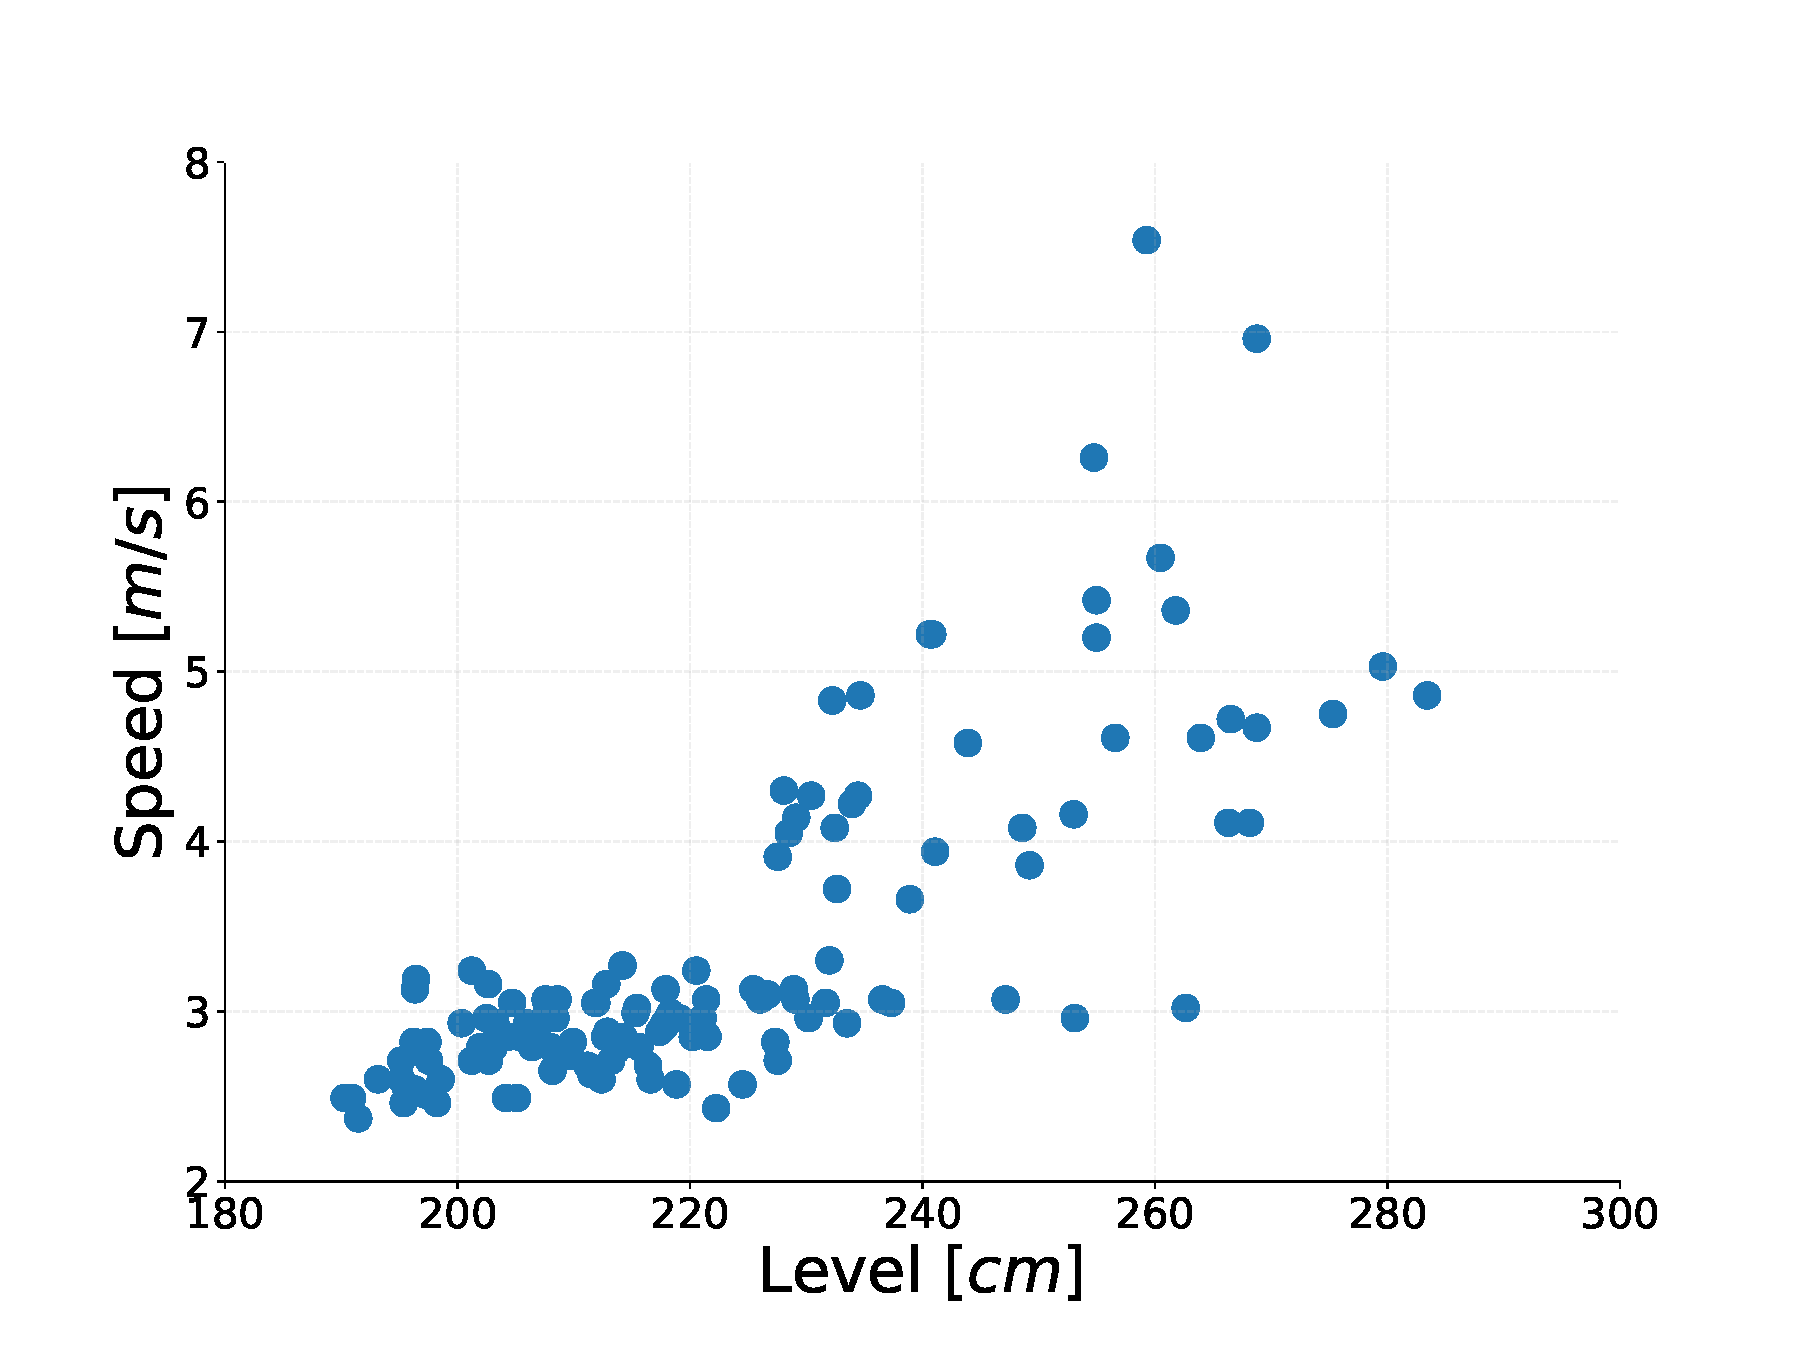
\includegraphics[width = 8cm]{Figures/level_speed_108.pdf}
\caption{\DIFaddFL{Scatter plot of water level (depth) (cm) and surface speed (ms$^{-1}$) for Doña María basin, located in the Aburrá Valley (Basin outlet coordinates: 75.651ºW, 6.190ºN). The basin slope is 34.09\%, the area :72.84 km$^2$, and the maximum (minimum) height is 2,835 m.a.s.l. (1,562 m.a.s.l.)}}
\label{fig:Appendix}
\end{figure}

%DIF >  

%DIF >  \subsection{}                               %% Appendix A1, A2, etc.
\DIFaddend 


%% REFERENCES
%% The reference list is compiled as follows:

%% Since the Copernicus LaTeX package includes the BibTeX style file copernicus.bst,
%% authors experienced with BibTeX only have to include the following two lines:
%%
\newpage
\bibliographystyle{copernicus}
%\bibliography{library.bib}
\bibliography{Flash_Floods.bib}
%%
%% URLs and DOIs can be entered in your BibTeX file as:
%%
%% URL = {http://www.xyz.org/~jones/idx_g.htm}
%% DOI = {10.5194/xyz}


%% LITERATURE CITATIONS
%%
%% command                        & example result
%% \citet{jones90}|               & Jones et al. (1990)
%% \citep{jones90}|               & (Jones et al., 1990)
%% \citep{jones90,jones93}|       & (Jones et al., 1990, 1993)
%% \citep[p.~32]{jones90}|        & (Jones et al., 1990, p.~32)
%% \citep[e.g.,][]{jones90}|      & (e.g., Jones et al., 1990)
%% \citep[e.g.,][p.~32]{jones90}| & (e.g., Jones et al., 1990, p.~32)
%% \citeauthor{jones90}|          & Jones et al.
%% \citeyear{jones90}|            & 1990

%% FIGURES

%% ONE-COLUMN FIGURES

%%f
%\begin{figure}[t]
%\includegraphics[width=8.3cm]{FILE NAME}
%\caption{TEXT}
%\end{figure}
%
%%% TWO-COLUMN FIGURES
%
%%f
%\begin{figure*}[t]
%\includegraphics[width=12cm]{FILE NAME}
%\caption{TEXT}
%\end{figure*}
%
%
%%% TABLES
%%%
%%% The different columns must be seperated with a & command and should
%%% end with \\ to identify the column brake.
%
%%% ONE-COLUMN TABLE
%
%%t
%\begin{table}[t]
%\caption{TEXT}
%\begin{tabular}{column = lcr}
%\tophline
%
%\middlehline
%
%\bottomhline
%\end{tabular}
%\belowtable{} % Table Footnotes
%\end{table}
%
%%% TWO-COLUMN TABLE
%
%%t
%\begin{table*}[t]
%\caption{TEXT}
%\begin{tabular}{column = lcr}
%\tophline
%
%\middlehline
%
%\bottomhline
%\end{tabular}
%\belowtable{} % Table Footnotes
%\end{table*}
%
%
%%% NUMBERING OF FIGURES AND TABLES
%%%
%%% If figures and tables must be numbered 1a, 1b, etc. the following command
%%% should be inserted before the begin{} command.
%
%\addtocounter{figure}{-1}\renewcommand{\thefigure}{\arabic{figure}a}
%
%
%%% MATHEMATICAL EXPRESSIONS
%
%%% All papers typeset by Copernicus Publications follow the math typesetting regulations
%%% given by the IUPAC Green Book (IUPAC: Quantities, Units and Symbols in Physical Chemistry,
%%% 2nd Edn., Blackwell Science, available at: http://old.iupac.org/publications/books/gbook/green_book_2ed.pdf, 1993).
%%%
%%% Physical quantities/variables are typeset in italic font (t for time, T for Temperature)
%%% Indices which are not defined are typeset in italic font (x, y, z, a, b, c)
%%% Items/objects which are defined are typeset in roman font (Car A, Car B)
%%% Descriptions/specifications which are defined by itself are typeset in roman font (abs, rel, ref, tot, net, ice)
%%% Abbreviations from 2 letters are typeset in roman font (RH, LAI)
%%% Vectors are identified in bold italic font using \vec{x}
%%% Matrices are identified in bold roman font
%%% Multiplication signs are typeset using the LaTeX commands \times (for vector products, grids, and exponential notations) or \cdot
%%% The character * should not be applied as mutliplication sign
%
%
%%% EQUATIONS
%
%%% Single-row equation
%
%\begin{equation}
%
%\end{equation}
%
%%% Multiline equation
%
%\begin{align}
%& 3 + 5 = 8\\
%& 3 + 5 = 8\\
%& 3 + 5 = 8
%\end{align}
%
%
%%% MATRICES
%
%\begin{matrix}
%x & y & z\\
%x & y & z\\
%x & y & z\\
%\end{matrix}
%
%
%%% ALGORITHM
%
%\begin{algorithm}
%\caption{?}
%\label{a1}
%\begin{algorithmic}
%?
%\end{algorithmic}
%\end{algorithm}
%
%
%%% CHEMICAL FORMULAS AND REACTIONS
%
%%% For formulas embedded in the text, please use \chem{}
%
%%% The reaction environment creates labels including the letter R, i.e. (R1), (R2), etc.
%
%\begin{reaction}
%%% \rightarrow should be used for normal (one-way) chemical reactions
%%% \rightleftharpoons should be used for equilibria
%%% \leftrightarrow should be used for resonance structures
%\end{reaction}
%
%
%%% PHYSICAL UNITS
%%%
%%% Please use \unit{} and apply the exponential notation


\end{document}